\documentclass[b5paper]{book}
\usepackage{ctex}
\usepackage[margin=0.8in]{geometry}
\geometry{top=2.5cm}
\usepackage{amsmath}
\usepackage{caption}
\usepackage{indentfirst}
\usepackage{graphicx}
\usepackage{subfigure}
\usepackage{amssymb}
\usepackage{cuted}
\usepackage{color}
\usepackage[dvipsnames]{xcolor}
\usepackage{fancyhdr}
\usepackage{xeCJK}
\usepackage{titlesec}
\usepackage{float}
\definecolor{titleBlue}{RGB}{30,59,150}
\titleformat{\chapter}[block]{\huge\bfseries\color{titleBlue}}{第 \thechapter 章}{1em}{}
\titleformat{\section}[block]{\Large\bfseries\color{titleBlue}}{\thesection}{1em}{}
\titleformat{\subsection}[block]{\large\bfseries\color{titleBlue}}{\thesubsection}{1em}{}
\titlespacing*{\section} {0pt}{10pt}{0pt}
% \renewcommand{\chaptermark}[1]{\markboth{第\,\thechapter\,章\quad #1}{}}

\pagestyle{fancy}
\renewcommand{\chaptermark}[1]{\markboth{\CJKfamily{hei} \color{titleBlue}{第 \thechapter 章\quad #1} }{}}
\renewcommand{\sectionmark}[1]{\markright{\CJKfamily{hei} \color{titleBlue}  \thesection \quad #1}{}}

\fancyhead{} % clear all fields
\fancyhead[LO]{\CJKfamily{hei} \bfseries \color{titleBlue}{\rightmark}}
\fancyhead[RO]{\CJKfamily{hei} \bfseries \color{titleBlue}  \thepage}
\fancyhead[LE]{\CJKfamily{hei} \bfseries \color{titleBlue}  \thepage}
\fancyhead[RE]{\CJKfamily{hei} \bfseries \color{titleBlue}{\leftmark}}

\fancyfoot{}

\renewcommand{\headrulewidth}{0pt}
\renewcommand{\footrulewidth}{0pt}


\setlength{\parindent}{2em}
\renewcommand {\thetable} {\thechapter{}.\arabic{table}}
\renewcommand {\thefigure} {\thechapter{}.\arabic{figure}}
\numberwithin{equation}{chapter}

\newcommand {\bx} {\boldsymbol{\mathrm{x}}}
\newcommand {\bw} {\boldsymbol{\mathrm{w}}}
\newcommand {\sfx} {\boldsymbol{\mathsf{x}}}
\newcommand {\sft} {\boldsymbol{\mathsf{t}}}
\newcommand {\sfy} {\boldsymbol{\mathsf{y}}}
\newcommand {\rmT} {\mathrm{T}}
\newcommand {\rmd} {\mathrm{d}}
\newcommand {\bfMu} {\boldsymbol{\mu}}
\newcommand {\bfAl} {\boldsymbol{\alpha}}
\newcommand {\bfSigma} {\boldsymbol{\Sigma}}
\newcommand {\bfLambda} {\boldsymbol{\Lambda}}
\newcommand {\bfPhi} {\boldsymbol{\Phi}}
\newcommand {\bfphi} {\boldsymbol{\phi}}
\newcommand {\bfeta} {\boldsymbol{\eta}}
\newcommand {\calD} {\mathcal{D}}
\newcommand {\calN} {\mathcal{N}}
\newcommand {\calR} {\mathcal{R}}
\newcommand {\insertline} {\noindent{\color{red} \rule[5pt]{\textwidth}{0.1em}}}

\author{张括嘉 \\ 东北大学机器人科学与工程学院}

\begin{document}
\title{Pattern Recognition and Machine Learning 中文版}
\date{}
% \maketitle
	\chapter{绪 \quad 论}
	\noindent\rule[0.25\baselineskip]{\textwidth}{1pt}
	\renewcommand {\thetable} {\thechapter{}.\arabic{table}}
	\renewcommand {\thefigure} {\thechapter{}.\arabic{figure}}

	\chapter{概率分布}
	\noindent\rule[0.25\baselineskip]{\textwidth}{1pt}
	\renewcommand {\thetable} {\thechapter{}.\arabic{table}}
	\renewcommand {\thefigure} {\thechapter{}.\arabic{figure}}
	\textnormal{
	\indent 在第1章中,我们看到了概率论在模式识别问题中扮演了核心的角色。现在我们会更详细地研究一些典型的概率分布和它们的性质。这些概率分布本身吸引了很多人的兴趣,同时也构成了很多复杂模型的基础,我们将在整本书中频繁使用这些概率分布。本章中介绍的概率分布同时也会让我们有机会在比较简单的模型下研究统计学中的一些重要概念,例如贝叶斯推断,而在后续的章节中还会研究更加复杂的情况。\\
	\indent 在本章中介绍的概率分布的作用,是在给定了随机变量$\bx$的有限观测集合$\bx_1,...,$\\$\bx_N$的情况下对概率分布$p(\bx)$进行建模。这个问题被称为密度估计(density extimation)。为了达到这个目的,我们假设数据点是独立同分布的。不过应该意识到,密度估计问题是一个病态的问题,因为对于一个数据集可能得到的概率分布有无穷多个。实际上,任何在数据点$\bx_1,...,\bx_2$处非零的分布$p(\bx)$都是潜在的候选分布。分布选择的问题与第1章中在多项式拟合问题中提及过的模型选择问题密切相关,是模式识别中的核心问题。\\
	\indent 我们从离散变量的二项分布(binomial distribution)和多项分布(multinomial distribution)以及连续变量的高斯分布(Gaussian distribution)开始。它们都是参数分布(parametric distribution)的典型代表,因为它们都是由一些可调节的参数所控制的,比如高斯分布中的均值和方差。为了将这样的模型应用于密度估计,我们需要根据数据集确定适当的参数值。在频率学派的观点中,通常是针对某些标准进行优化(例如似然函数)来确定参数的值。与之不同的是,在贝叶斯学派的观点中,我们会引入参数的先验分布,然后利用贝叶斯定理,结合训练数据,计算对应的后验分布。\\
	\indent 我们将看到共轭先验(conjugate prior)即将发挥重要的作用,它可以使后验分布具有与先验相同的函数形式,使贝叶斯分析变得更加简单。举例而言,多项分布中参数的共轭先验被称为狄利克雷分布(Dirichlet distribution),高斯分布中均值的共轭先验则是另一个高斯分布。这些分布都共同属于指数型分布族(exponential family of distributions),它们具有很多重要的性质,我们会在后续内容中详细讨论。\\
	\indent 而参数方法也有无法回避的自身缺陷,那就是必须对分布假设一个具体的函数形式,而这个函数形式是否适合于实际应用却是无法保证的。在非参数密度估计(nonparametric density estimation)中,分布的形式仅仅取决于训练集的大小。尽管这样的模型同样也是含有参数的,但这些参数仅仅控制了模型的复杂度,而非分布的形式。我们会在章节的末尾研究3种非参数方法,分别是直方图方法、最近邻方法和核方法。
	}
	\section{二元变量}
	\insertline
	\textnormal{
	\indent 我们从最简单的二元随机变量$x \in \{0,1\}$开始。举例而言,$x$表示的可能是投掷一枚硬币的结果,$x=1$表示正面,$x=0$表示反面。我们也可以想象这个硬币有可能遭到了破坏,正面向上的概率和反面向上的概率不一定是相同的。$x=1$的概率表示为参数$\mu$,于是
	\begin{equation}
		p(x=1|\mu)=\mu
	\end{equation}
	其中$0 \leqslant \mu \leqslant 1$。于是也可以得到$p(x=0|\mu) = 1-\mu$。那么$x$的概率分布就可以写成
	\begin{equation}
		\mathrm{Bern}(x|\mu)=\mu^x(1-\mu)^{1-x} 
	\end{equation}
	这就是著名的伯努利分布(Bernoulli distribution)。可以很容易地验证这个分布满足归一化条件,而且其均值和方差分别为\textcolor{red}{\textbf{——习题 2.1}}
	\begin{align}
		\mathbb{E}[x]&=\mu \\
		\mathrm{var}[x]&=\mu(1-\mu)
	\end{align}
	\indent 现在假设我们有一个$x$的数据集$\mathcal{D}=\{x_1,...,x_N\}$。假设各个数据都是从分布$p(x|\mu)$中相互独立地获取的,那么可以构建似然函数,这个似然函数实际上是一个关于$\mu$的函数
	\begin{equation}
		p(\mathcal{D}|\mu)=\prod_{n=1}^{N}p(x_n|\mu)=\prod_{n=1}^N\mu^{x_n}(1-\mu)^{1-x_n}
	\end{equation}
	在频率学派观点中,我们可以通过对似然函数,或者对与之等价的对数似然函数进行最大化来估计$\mu$的值。对于伯努利分布,对数似然函数为
	\begin{equation}
		\ln p(\mathcal{D}|\mu) = \sum_{n=1}^N\ln p(x_n|\mu) = \sum_{n=1}^N \{x_n \ln \mu + (1-x_n)\ln(1-\mu)\}
	\end{equation}
	此时应该注意到,对数似然函数对这$N$个$x_n$的依赖不过是对其总和$\sum_n x_n$的依赖而已。这个总和是这一分布下数据的充分统计量(sufficient statistic),充分统计量是很重要的概念,我们会在后续内容中详细介绍。\textcolor{red}{\textbf{——第2.4节\ }}如果令$\ln p(\mathcal{D}|\mu)$关于$\mu$的导数等于0,那么最大似然估计就是
	\begin{equation}
		\mu_{\mathrm{ML}}=\frac{1}{N}\sum_{n=1}^N x_n
	\end{equation}
	这个值也被称为样本均值(sample mean)。如果这个数据集中,$x=1$(也就是正面向上)的数据共有$m$个,那么(2.7)就可以写成
	\begin{equation}
		\mu_{\mathrm{ML}} = \frac{m}{N}
	\end{equation}
	这就是正面向上的概率。在最大似然中,正面向上的概率是完全根据训练集中正面向上的比例确定的。\\
	\indent 现在假设我们抛了3次硬币,而且恰好3次全是正面向上,那么$N=m=3$,$\mu_{\mathrm{ML}}=1$。在这种情况下,最大似然方法会给出这样的结果——不管怎么抛硬币,一定是正面向上。然而稍有常识的人都会看出,如果我们的实验继续前进,这个螳臂当车的预测肯定是图样图森破的。这就是最大似然方法中典型的过拟合现象。我们很快就会看到引入$\mu$的先验分布可以得到更加合理的结果。\\
	\indent 我们同样可以在给定了数据集大小$N$的情况下确定$m$的分布,$m$仍然表示$x=1$的数据数量。这就是二项分布。根据(2.5),可以看出这个分布是与$\mu^m (1-\mu)^{N-m}$成正比。接下来确定归一化系数,假设抛了$N$次硬币,把所有出现$m$次正面的情况全加起来,那么二项分布就可以写成
	\begin{equation}
		\mathrm{Bin}(m|N,\mu)=\left(\begin{matrix} N \\ m \end{matrix} \right) \mu^m(1-\mu)^{N-m}
	\end{equation}
	其中
	\begin{equation}
		\left( \begin{matrix} N \\ m \end{matrix} \right) \equiv \frac{N!}{(N-m)!m!}
	\end{equation}
	表示$N$次抛掷中出现$m$次正面的所有可能。\textcolor{red}{\textbf{——习题 2.3}\ }图2.1表示的是$N=10$和$\mu=0.25$的二项分布示意图。
	\begin{figure}[ht]
		\centering
		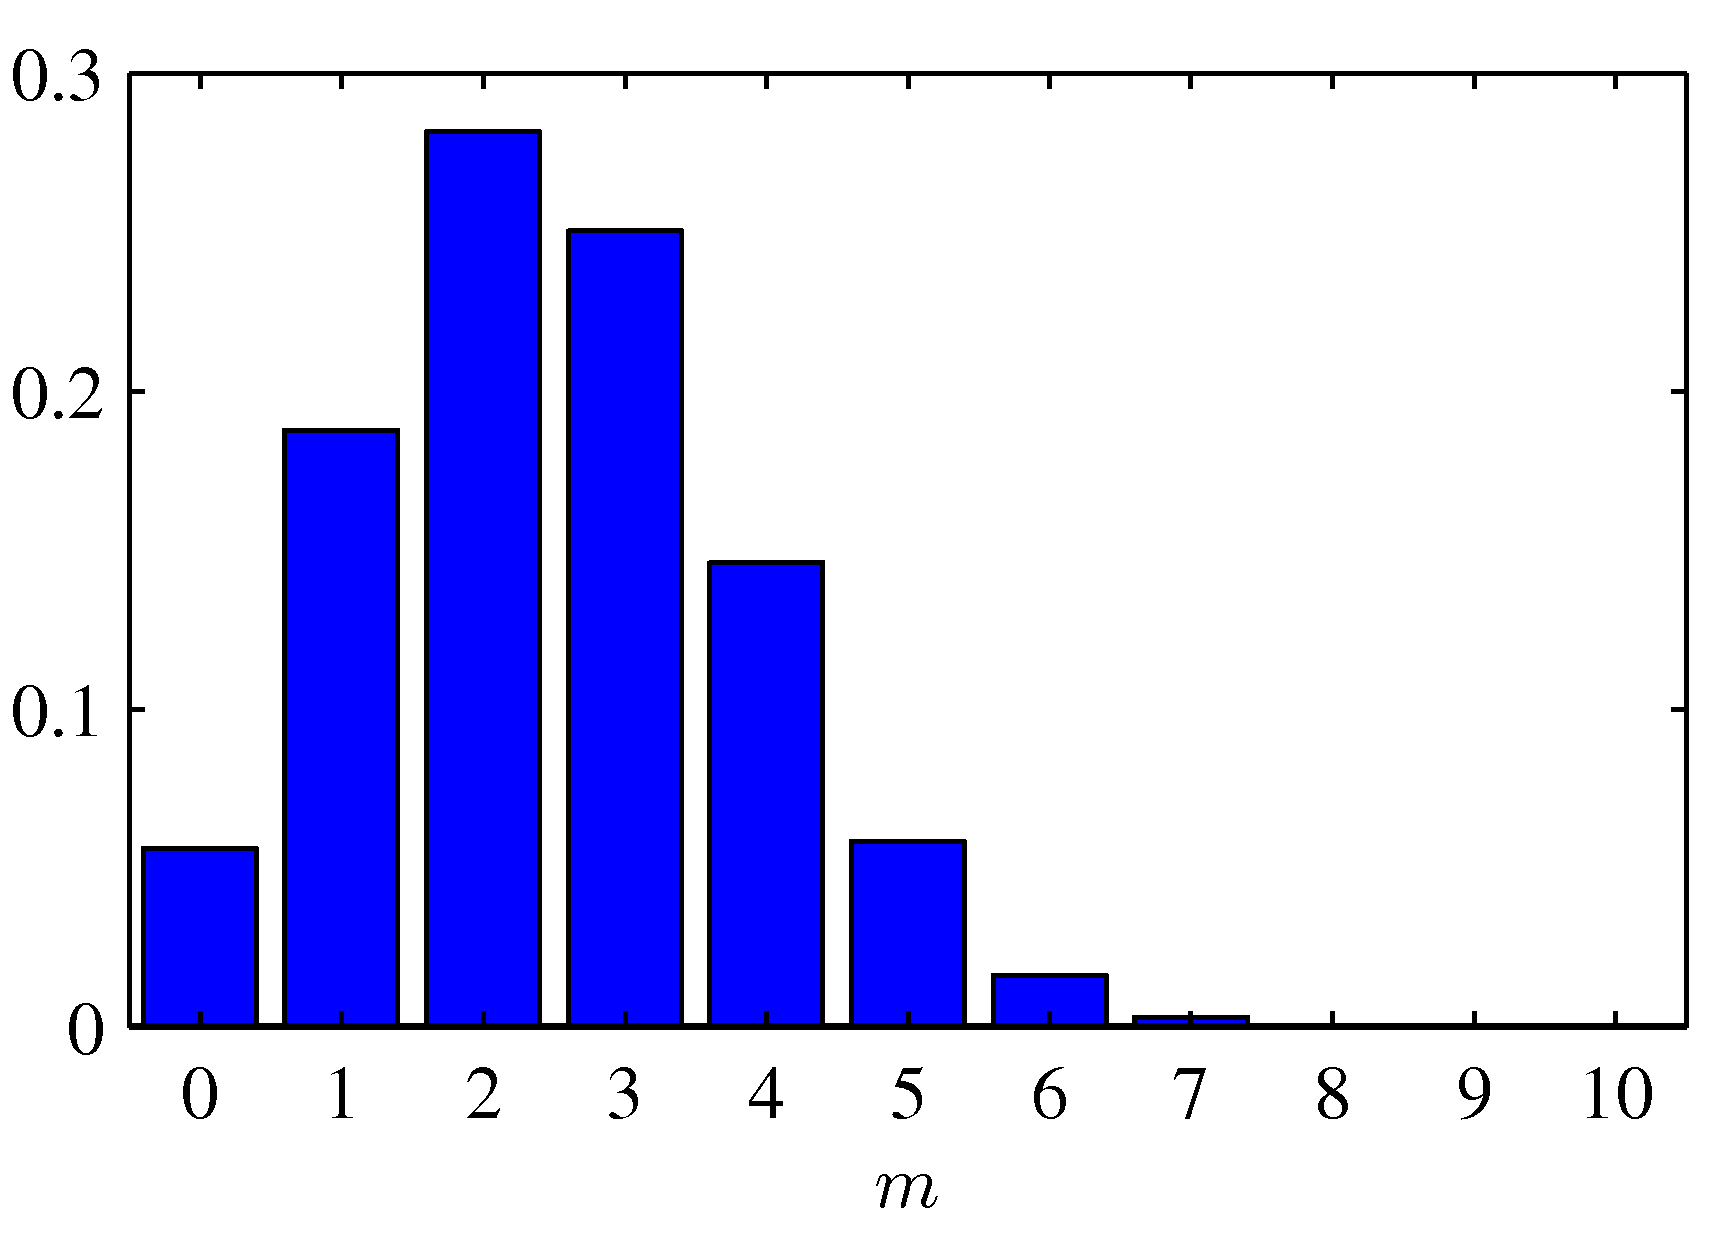
\includegraphics[scale=0.8]{Images/2-1.png}
		\captionsetup{font={small}}
		\caption{二项分布(2.9)在$N=10$和$\mu=0.25$时关于$m$的直方图。}
		\label{fig:2-1}
	\end{figure}
	\\
	\indent 二项分布的均值和方差可以通过习题1.10的结论求出,也就是对于独立事件而言,其总和的均值就是均值的总和,总和的方差就是方差的总和。由于$m=x_1+...+x_N$,而且数据集中每个元素的均值和方差都由(2.3)和(2.4)给出了,那么
	\begin{align}
		\mathbb{E}[m] \equiv \sum_{m=0}^{N}m \mathrm{Bin}(m|N,\mu) &= N\mu \\
		\mathrm{var}[m] \equiv \sum_{m=0}^N(m-\mathbb{E}[m])^2\mathrm{Bin}(m|N,\mu) &= N\mu(1-\mu)
	\end{align}
	这两个结果也可以直接计算得到。\textcolor{red}{\textbf{——习题 2.4}}
	}
	\subsection{beta分布}
	\textnormal{在(2.8)中我们已经看到了求伯努利分布参数$\mu$的最大似然的方法,所以在二项分布中参数$\mu$的最大似然是根据数据集中$x=1$的数据在数据集中所占的比例来确定的。我们已经发现了在较小的数据集上这种方法可能会造成过拟合的现象。为了对这个问题进行贝叶斯风格的处理,我们需要引入一个参数$\mu$的先验分布$p(\mu)$。在这里,我们需要的是一个比较简单,又有很多实用性质的先验分布。为了得到这个先验,我们首先注意到似然函数的形式是一系列因子$\mu^x(1-\mu)^{1-x}$的乘积。如果我们选择的是类似形式的先验,而先验分布与似然函数求乘积之后又和后验分布仅相差一个系数,那么后验分布就与先验分布具有相同的形式了。这样的性质称为共轭(conjugacy),在本章后面的内容中会看到共轭的相关案例。于是我们选择了这样的一个先验,起个名字叫做beta分布,形式为\\
	\begin{equation}
		\mathrm{Beta}(\mu|a,b)=\frac{\Gamma(a+b)}{\Gamma(a)\Gamma(b)}\mu^{a-1}(1-\mu)^{b-1}
	\end{equation}
	其中的$\Gamma(x)$为Gamma函数,定义详见(1.141)。(2.13)中的常数使beta分布满足归一化条件,\textcolor{red}{\textbf{——习题 2.5}}\ 也就是说
	\begin{equation}
		\int_0^1\mathrm{Beta}(\mu|a,b)\ \mathrm{d}\mu =1
	\end{equation}
	beta分布的均值和方差分别为\textcolor{red}{\textbf{——习题 2.6}}
	\begin{align}
		\mathbb{E}[\mu]&=\frac{a}{a+b} \\
		\mathrm{var}[\mu]&=\frac{ab}{(a+b)^2(a+b+1)}
	\end{align}
	其中的参数$a$和$b$被称为超参数(hyperparameters),因为它们把控着分布的参数$\mu$。如图2.2所示为超参数取不同值时的beta分布。
	\begin{figure}[ht]
		\begin{minipage}[t]{0.5\linewidth}
		\centering
		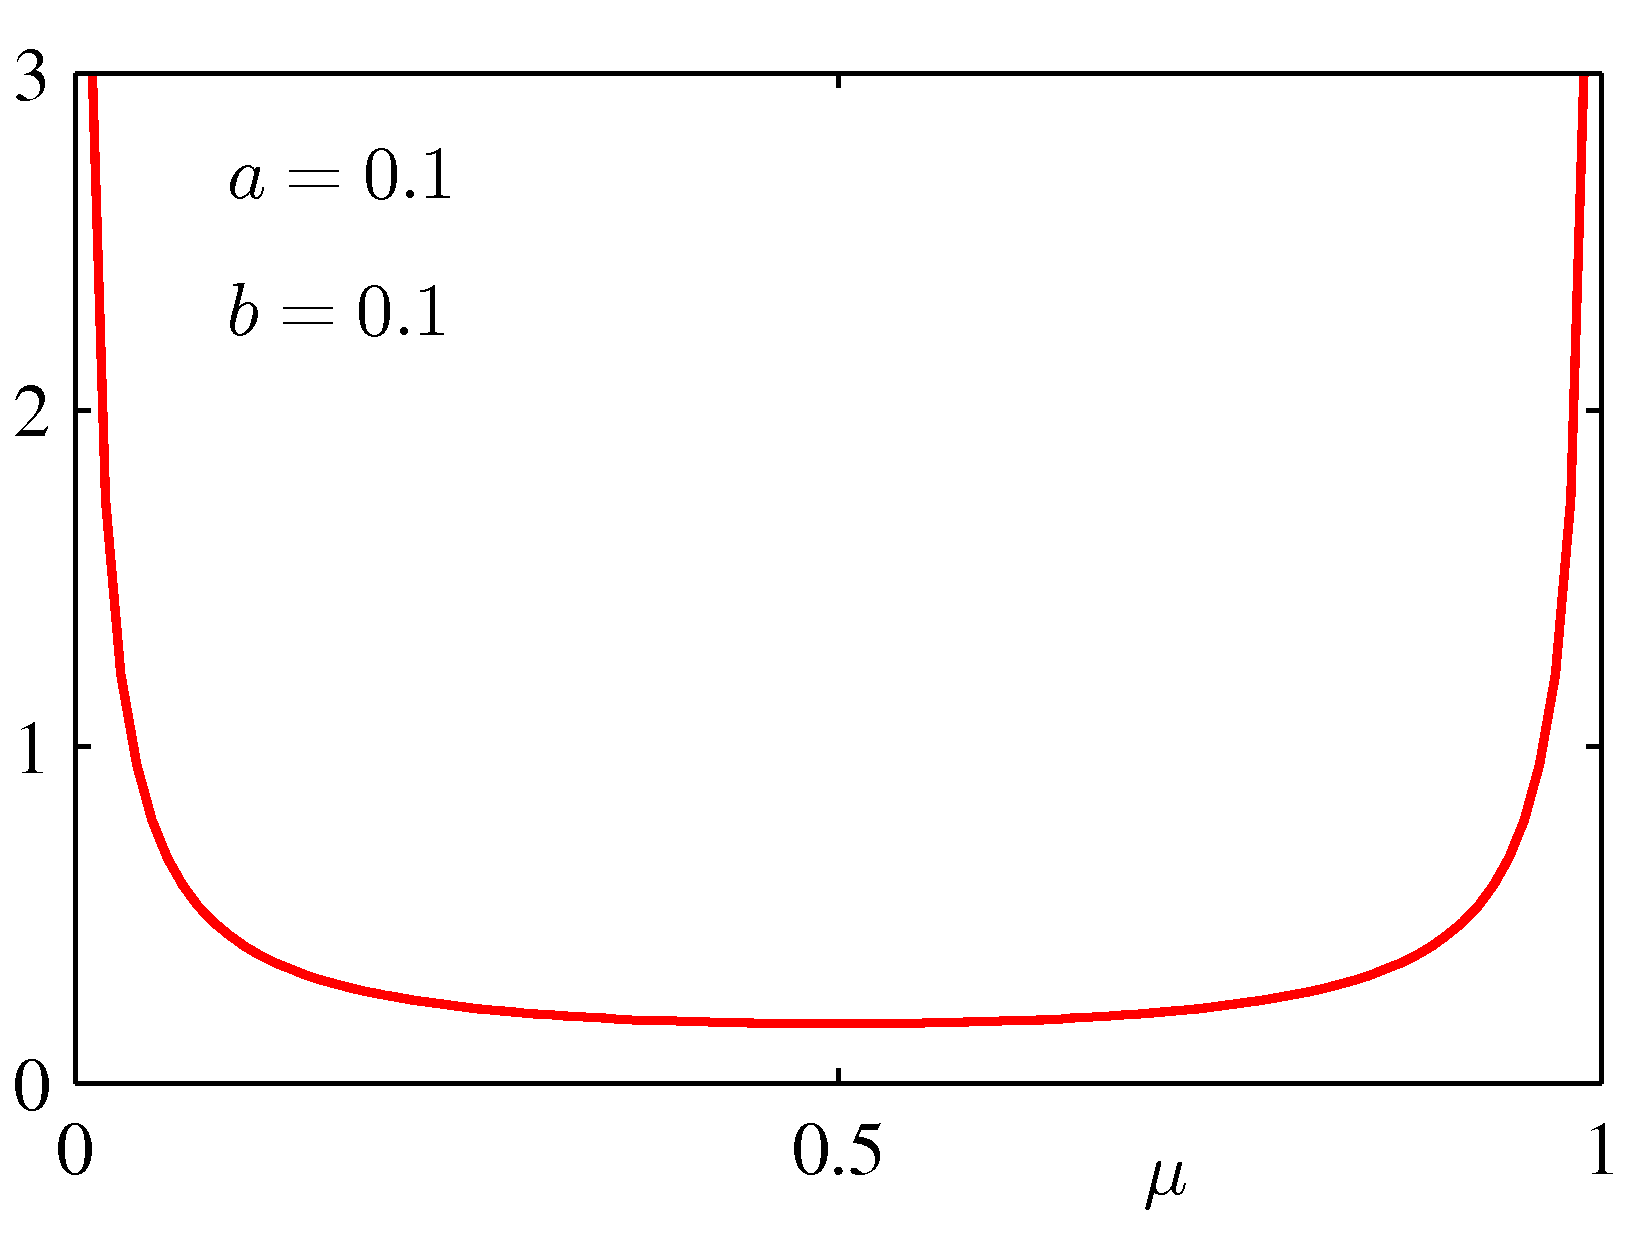
\includegraphics[scale=0.8]{Images/2-2a.png}
		\label{fig:2-2a}
		\end{minipage}
		\begin{minipage}[t]{0.5\linewidth}
		\centering
		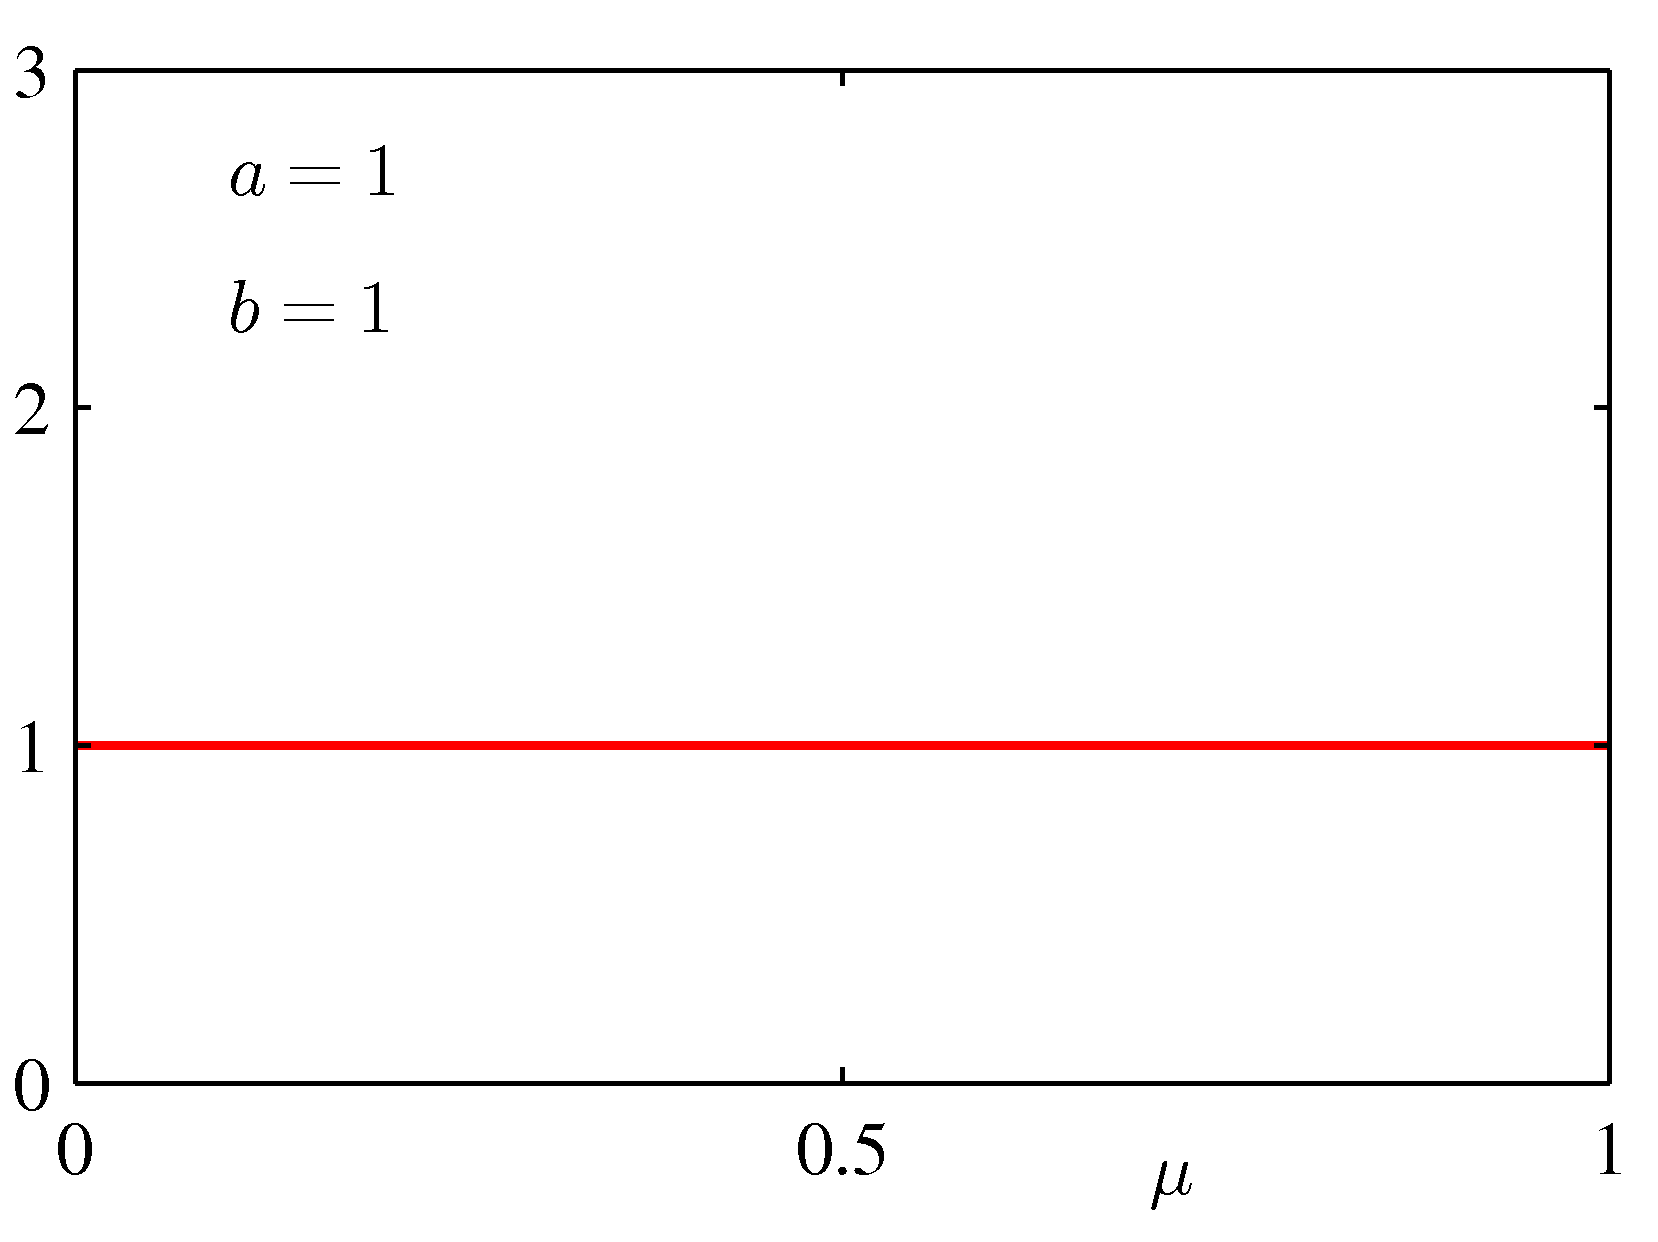
\includegraphics[scale=0.8]{Images/2-2b.png}
		\label{fig:2-2b}
		\end{minipage}\\
		\begin{minipage}[t]{0.5\linewidth}
		\centering
		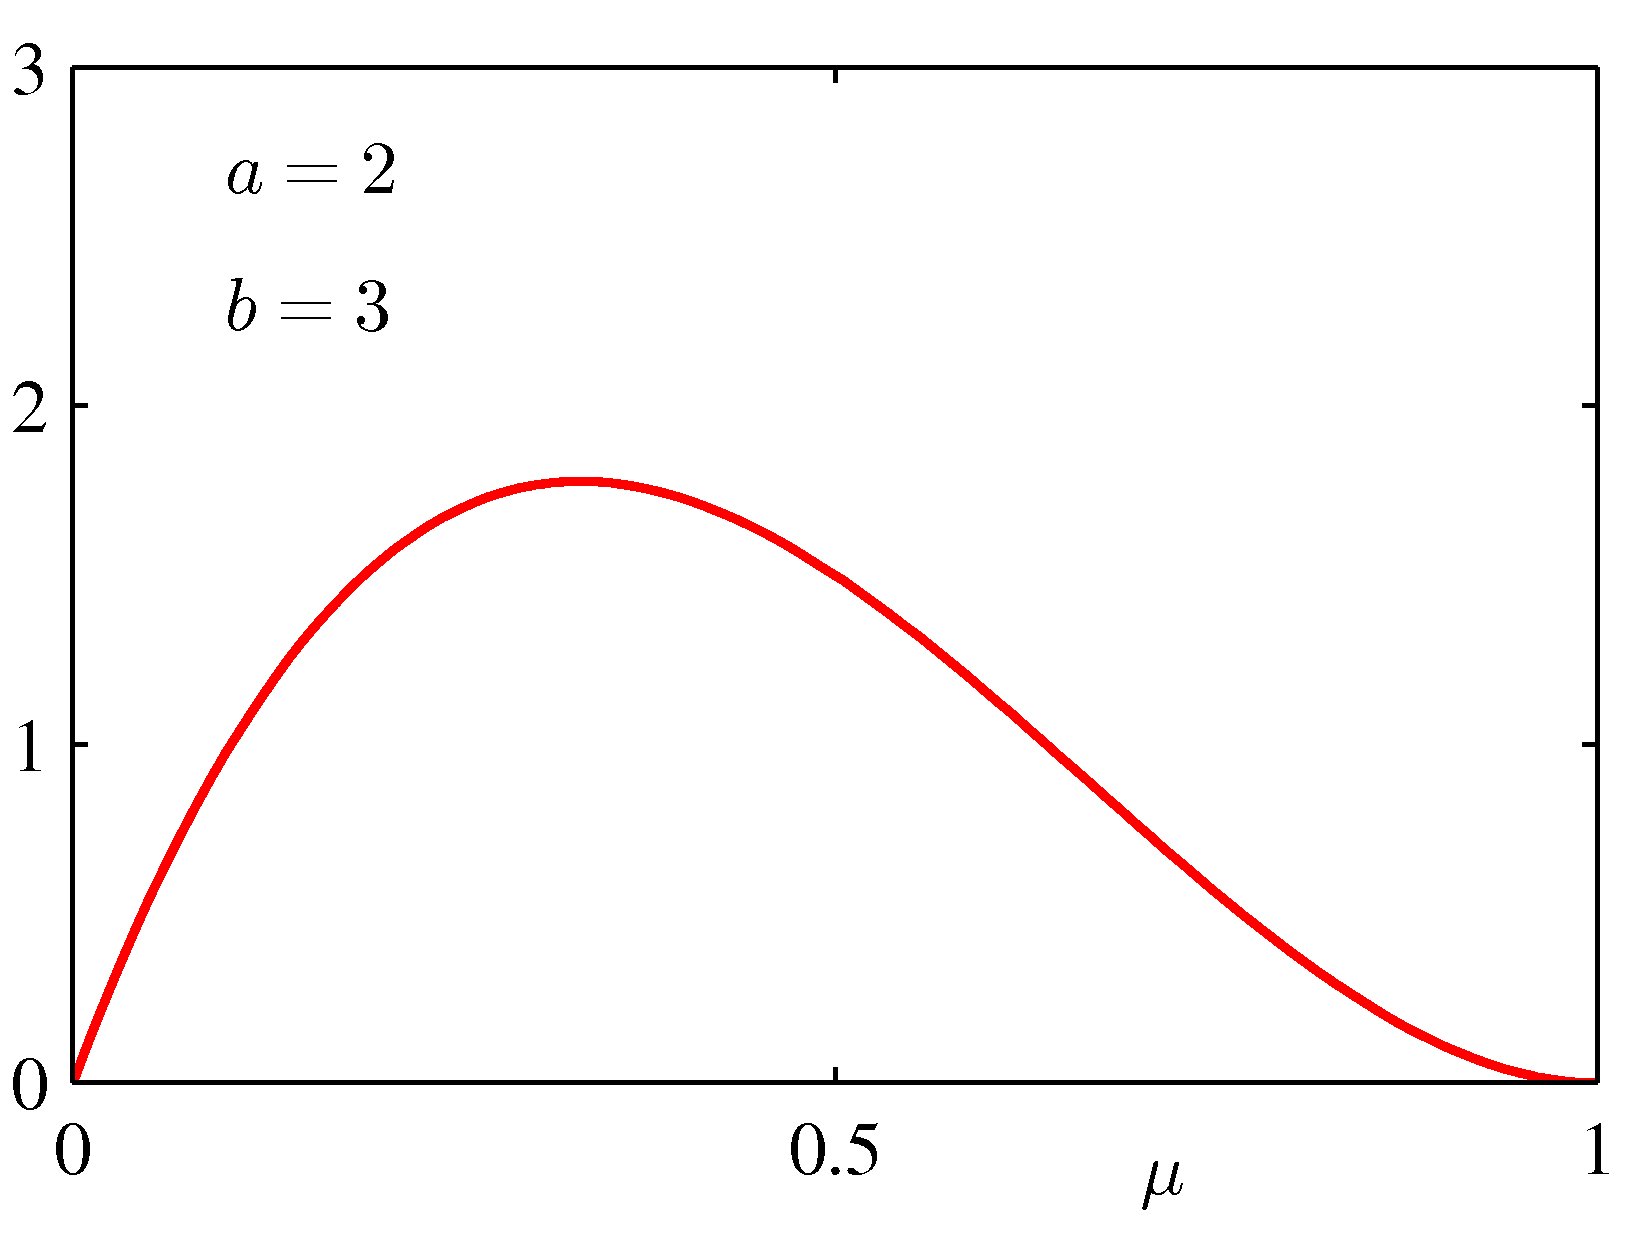
\includegraphics[scale=0.8]{Images/2-2c.png}
		\label{fig:2-2c}
		\end{minipage}
		\begin{minipage}[t]{0.5\linewidth}
		\centering
		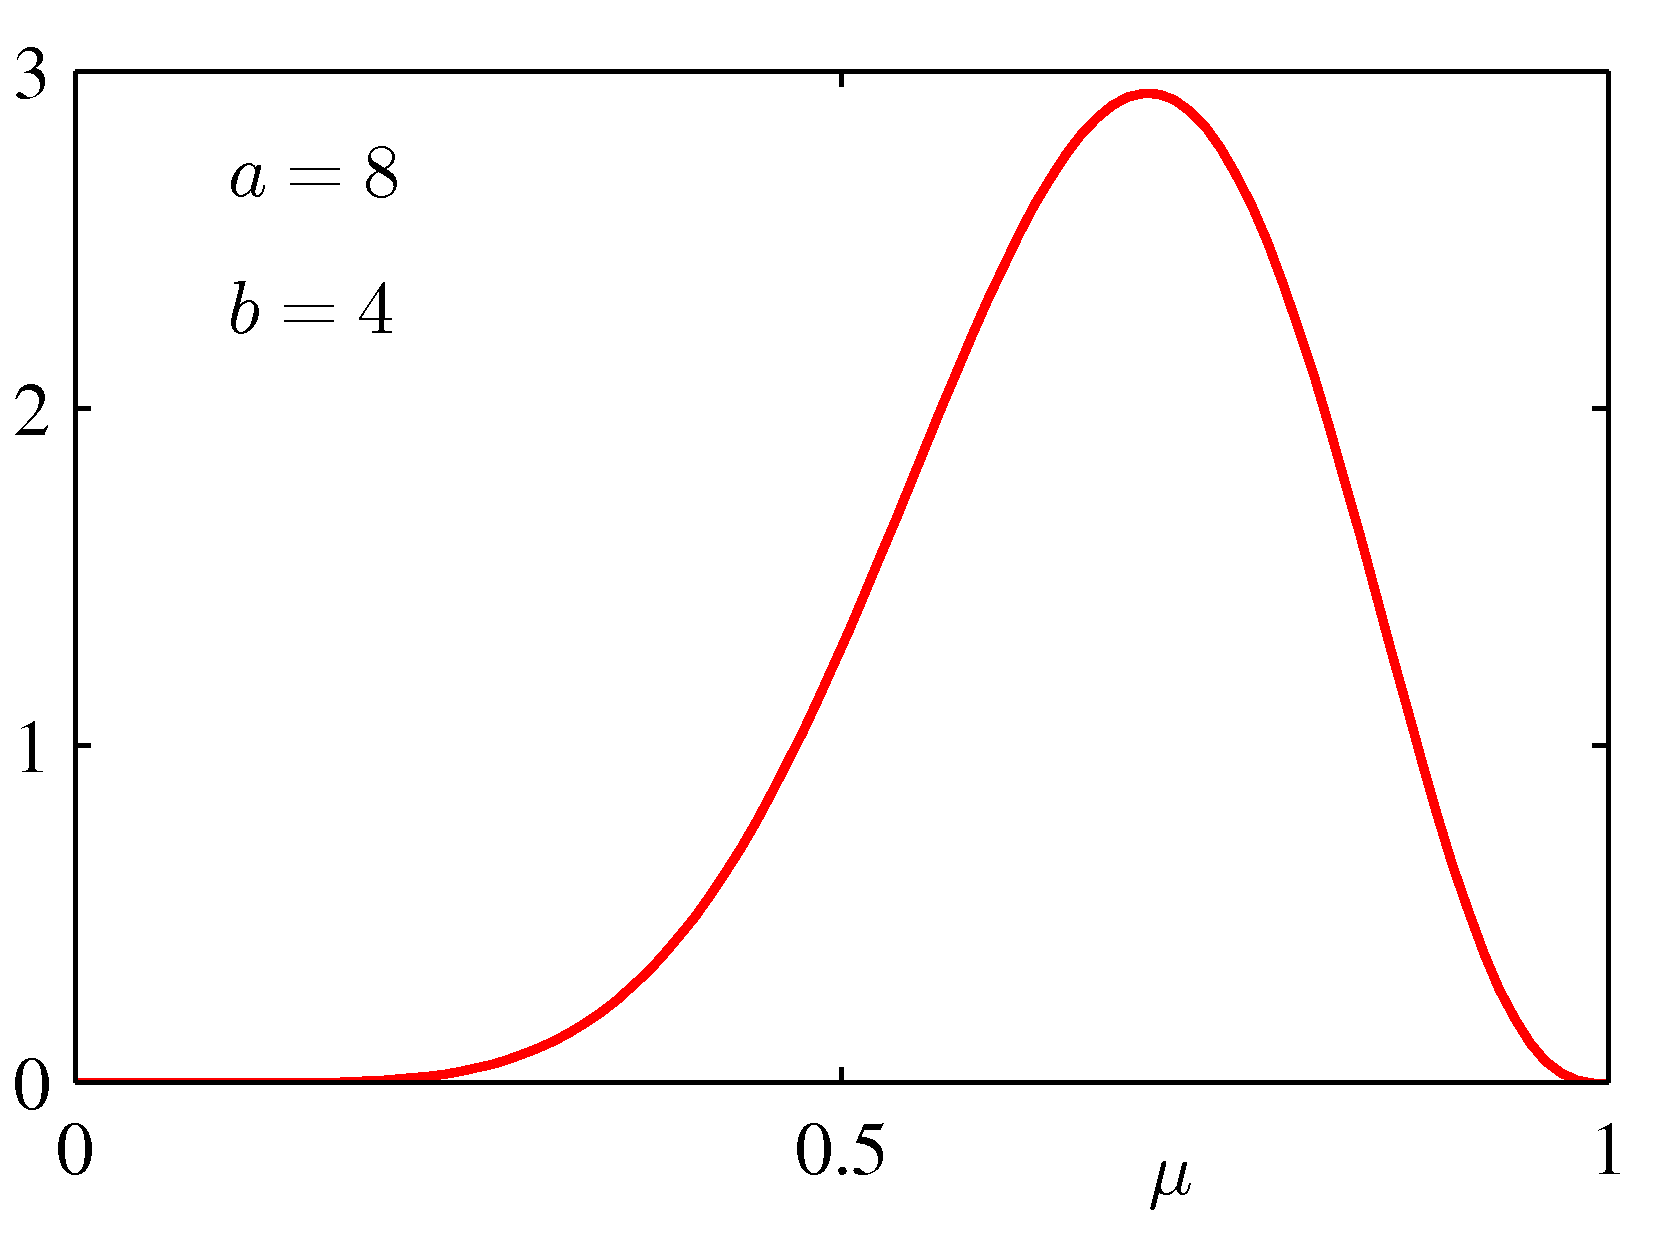
\includegraphics[scale=0.8]{Images/2-2d.png}
		\label{fig:2-2d}
		\end{minipage}
		\captionsetup{font={small}}
		\caption{在不同的超参数$a$,$b$下,(2.13)中的beta分布$\mathrm{Beta}(\mu|a,b)$关于$\mu$的函数图像。}
	\end{figure}
	\\
	\indent 现在可以将beta分布(2.13)作为先验,乘以二项似然函数(2.9)并进行归一化,从而得到$\mu$的后验分布。仅保留与$\mu$相关的因子,可以看出后验分布为如下形式:
	\begin{equation}
		p(\mu|m,l,a,b) \propto \mu^{m+a-1}(1-\mu)^{l+b-1}
	\end{equation}
	其中$l=N-m$,所以就与背面朝上的次数挂上关系了。可以看出,作为$\mu$的函数,(2.17)的形式与先验分布的形式是相同的,也反映了先验分布与似然函数之间的共轭性质。实际上这就是另一个beta分布,通过与(2.13)做一下对比就可以写出其归一化常数:
	\begin{equation}
		p(\mu|m,l,a,b)=\frac{\Gamma(m+a+l+b)}{\Gamma(m+a)\Gamma(l+b)}\mu^{m+a-1}(1-\mu)^{l+b-1}
	\end{equation}
	\indent 可以看出,数据集会在先验分布转化为后验分布的过程中产生影响,如果$x=1$的观测数量为$m$,$x=0$的观测数量为$l$,那么$a$就会增加$m$,$b$会增加$l$。这就使得我们可以将超参数$a$和$b$比较简单地解释为$x=1$和$x=0$的有效数据量(effective number of observations)。注意,$a$和$b$可以不是整数。另外,如果我们还有后续的新数据,那么后验分布就可以成为下一步的先验分布。为了看清楚这一点,我们可以想象在每次数据观测之后都更新当前的后验分布,更新的方式为,将后验分布与新观测的似然函数相乘并进行归一化后,得到进一步修正的新后验分布。在每一步中,后验分布都是带有超参数$a$和$b$的beta分布,超参数$a$和$b$分别表示$x=1$和$x=0$的数量。如果有一个新的$x=1$加入进来,就直接将$a$值加上1即可,同理,如果有一个新的$x=0$加入进来,那就直接将$b$的值加上1。图2.3展示了这一过程,也就是获得一个新的数据时对分布进行的修正。
	\begin{figure}[ht]
	\centering
		\begin{minipage}[t]{0.3\linewidth}
		\centering
		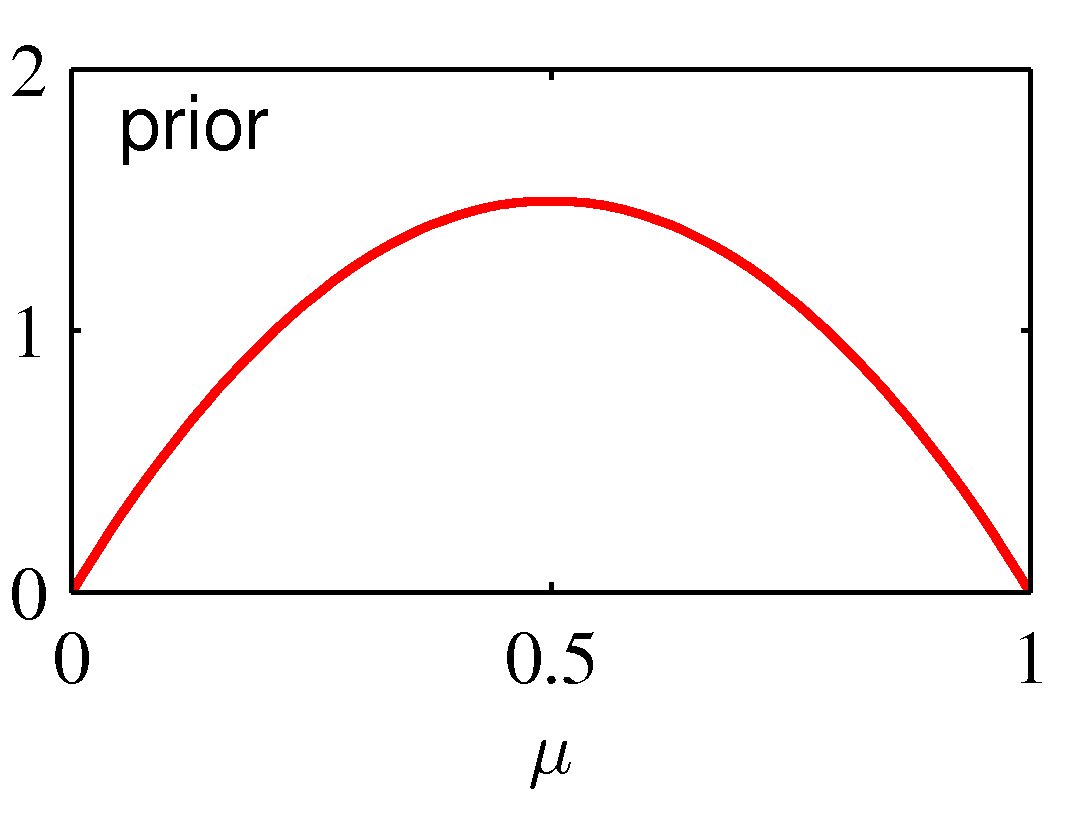
\includegraphics[scale=0.8]{Images/2-3a.png}
		\label{fig:2-3a}
		\end{minipage}
		\begin{minipage}[t]{0.3\linewidth}
		\centering
		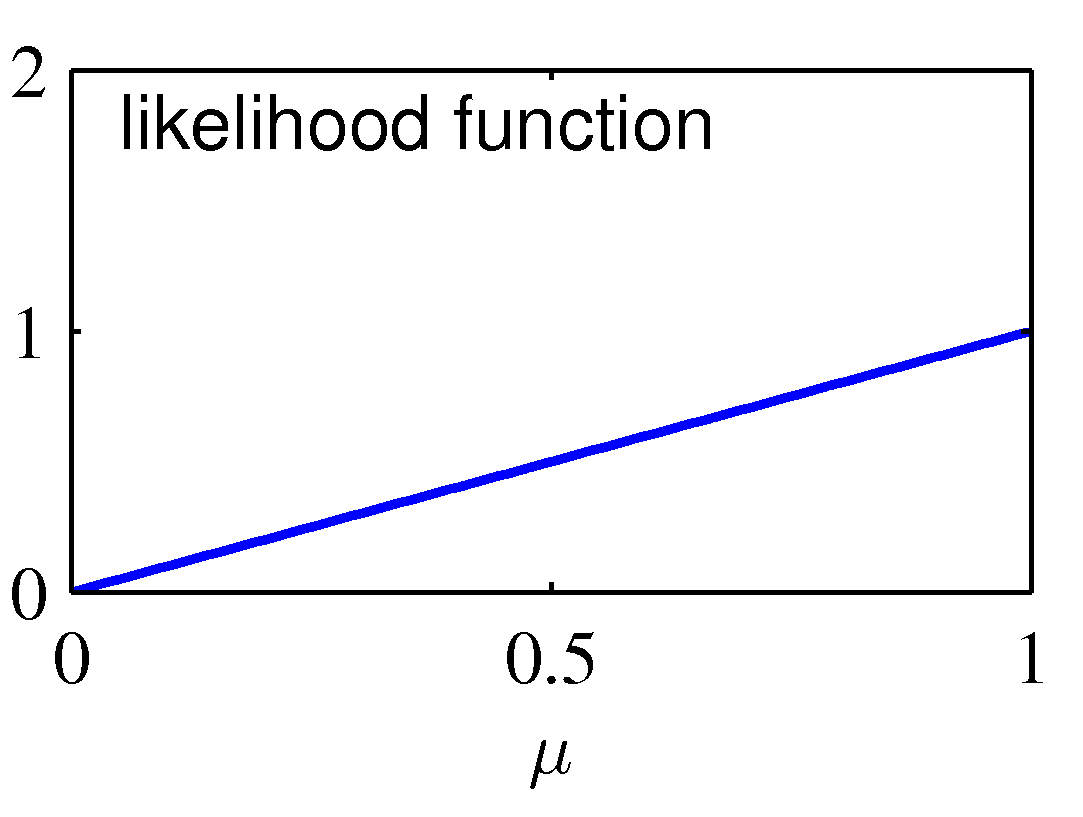
\includegraphics[scale=0.8]{Images/2-3b.png}
		\label{fig:2-3b}
		\end{minipage}
		\begin{minipage}[t]{0.3\linewidth}
		\centering
		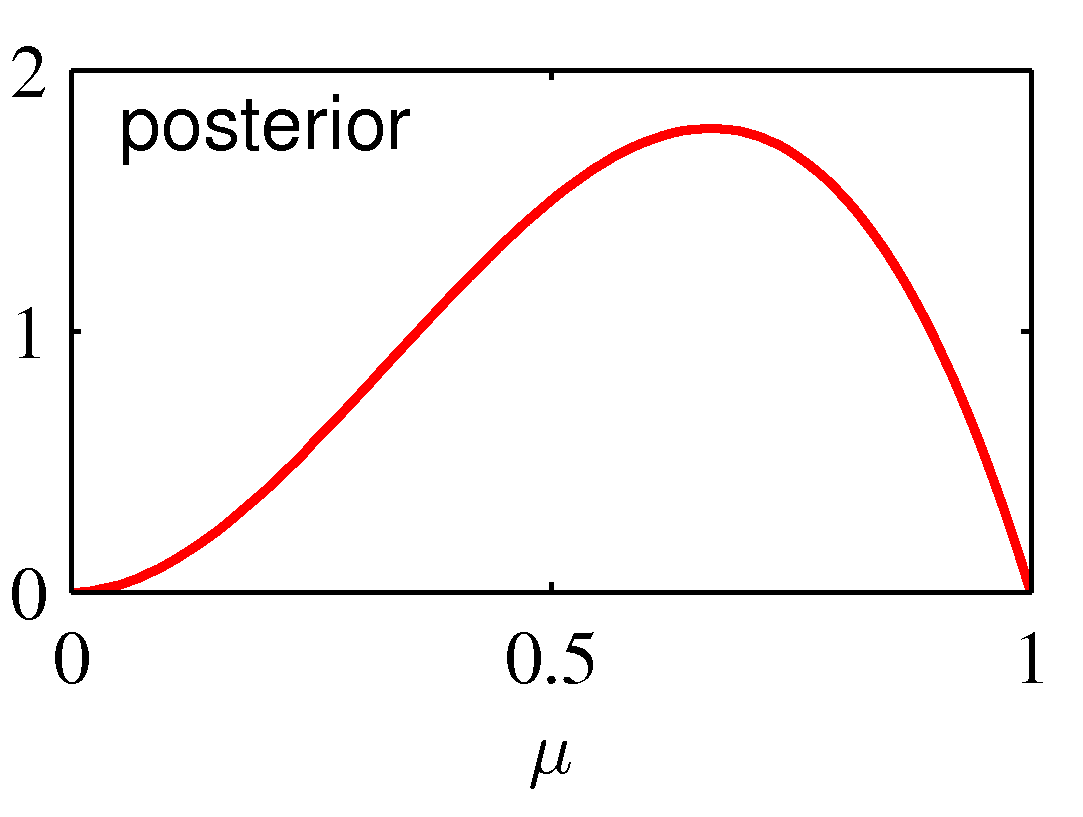
\includegraphics[scale=0.8]{Images/2-3c.png}
		\label{fig:2-3c}
		\end{minipage}
		\captionsetup{font={small}}
		\caption{贝叶斯推断过程中的一次分布更新。先验beta分布的超参数$a=2$,$b=2$,似然函数如(2.9)所示,其中的$N=m=1$,也就是拿到了一个新的$x=1$的数据,于是后验beta分布的超参数就是$a=3$,$b=2$了。}
	\end{figure}
	\\
	\indent 可以看出,如果使用贝叶斯观点,那么可以自然而然地形成这种“顺序”(sequential)的学习方法。它与我们所选择的先验分布和似然函数无关,而是仅仅与数据的独立同分布假设相关。随着顺序方法的一步步推进,在每一步中都会利用单个或者小批量的数据,然后在使用下一个观测数据进行更新之前将它们废弃。举例而言,在实时学习的场合中,我们要在数据以稳定的数据流的形式到达之后对之逐一加以利用,而且要在全部数据到达之前进行预测。由于不需要将完整的数据集都存储或加载到内存中,所以顺序方法也经常应用于大型的数据集中。另外,最大似然方法实际上也可以转化为顺序框架的形式。\textcolor{red}{\textbf{——第2.3.5节}}\\
	\indent 如果我们的目标是尽可能准确地预测下一次试验的结果,那我们就必须对给定数据集$D$的条件下$x$的预测分布进行评价。根据概率论中的加法和乘法规则,有如下等式:
	\begin{equation}
		p(x=1|\mathcal{D})=\int_0^1p(x=1|\mu)p(\mu|\mathcal{D})\ \mathrm{d}\mu = \int_0^1 \mu p(\mu|\mathcal{D})\ \mathrm{d}\mu = \mathbb{E}[\mu|\mathcal{D}]
	\end{equation}
	利用(2.18)中的结果,结合(2.15)中的关于beta分布均值的结论,对于后验分布$p(\mu|\mathcal{D})$,有:
	\begin{equation}
		p(x=1|\mathcal{D})=\frac{m+a}{m+a+l+b}
	\end{equation}
	这个等式的意义很简单,实际上就是$x=1$的数据数量占数据总数的比例。需要注意的是,对于无限大的数据集,$m,l \rightarrow \infty$,(2.20)就退化成了(2.8)中的最大似然结果。我们即将看到,贝叶斯方法和最大似然方法的结果在数据集趋向于无限大时其实是一致的,这是一条非常重要的性质。而在有限数据集中,$\mu$的后验均值总是处于先验均值与最大似然结果之间,最大似然结果对应的是(2.7)所给出的事件相对频率。\textcolor{red}{\textbf{——习题 2.7}}\\
	\indent 从图2.2中可以看出,随着数据数量的增加,后验分布会变得越来越陡峭。也可以从(2.16)中看出一些端倪,当$a \rightarrow \infty$或$b \rightarrow \infty$时,方差会趋向于0。实际上,我们希望知道这是不是贝叶斯学习的一般属性之一,即当我们获得越来越多的数据之后,后验分布所代表的不确定性会不会逐步地下降。\\
	\indent 为了验证这一点,我们可以从频率域的角度来审视贝叶斯学习,并证明在一般情况下这个性质确实是成立的。让我们设想一个一般的贝叶斯推断问题,我们要根据数据集$\mathcal{D}$推断参数$\boldsymbol{\theta}$,其关系由联合分布$p(\boldsymbol{\theta},\mathcal{D})$来描述。以下结果\textcolor{red}{\textbf{——习题 2.8}}
	\begin{equation}
		\mathbb{E}_{\boldsymbol{\theta}}[\boldsymbol{\theta}]=\mathbb{E}_{\mathcal{D}}[\mathbb{E}_{\boldsymbol{\theta}}[\boldsymbol{\theta}|\mathcal{D}]]
	\end{equation}
	其中
	\begin{align}
		\mathbb{E}_{\boldsymbol{\theta}}[\boldsymbol{\theta}] &\equiv \int p(\boldsymbol{\theta})\boldsymbol{\theta}\ \mathrm{d}\boldsymbol{\theta} \\
		\mathbb{E}_{\mathcal{D}}[\mathbb{E}_{\boldsymbol{\theta}}[\boldsymbol{\theta}|\mathcal{D}]] &\equiv \int \left\{\int \boldsymbol{\theta} p(\boldsymbol{\theta}|\mathcal{D})\ \mathrm{d}\boldsymbol{\theta} \right\}p(\mathcal{D})\ \mathrm{d}\mathcal{D}
	\end{align}
	表明,基于全部数据取平均值的$\boldsymbol{\theta}$的后验均值与其先验均值相等。类似地,我们也可以证明
	\begin{equation}
		\mathrm{var}_{\boldsymbol{\theta}}[\boldsymbol{\theta}]=\mathbb{E}_{\mathcal{D}}[\mathrm{var}_{\boldsymbol{\theta}}[\boldsymbol{\theta}|\mathcal{D}]] + \mathrm{var}_{\mathcal{D}}[\mathbb{E}_{\boldsymbol{\theta}}[\boldsymbol{\theta}|\mathcal{D}]]
	\end{equation}
	等式(2.24)的等号左侧为$\boldsymbol{\theta}$的先验方差。在等号右侧,第一项为$\boldsymbol{\theta}$的平均后验方差,第二项衡量的是$\boldsymbol{\theta}$后验期望的方差。由于这个方差是个非负数,所以这个结果的含义是,在一般情况下,$\boldsymbol{\theta}$的后验方差小于先验方差。如果后验均值的方差比较大,那么方差减小的量会变得更大。不过需要注意的是,这个结论仅在一般情况下适用,对于很特殊的数据集,那么还是有可能出现后验方差大于先验方差的情况的。
	}
	\section{多项变量}
	\insertline
	\textnormal{
	\indent 二元变量可以描述变量有一种或者两种取值的情况。不过通常,我们面对的离散变量可能会有$K$种取值,且每种取值之间是互斥的。有很多方式来表达这样的变量,其中一种特别方便的办法叫做1-of-K方法,我们很快就会用到它。这个方法中,每个变量都表示为$K$维向量$x$,其中有且仅有一个分量$x_k=1$,其余均为0。于是,假设我们有个$K=6$的随机变量,而且要表示$x_3=1$的状态,那么直接可以写成
	\begin{equation}
		\bx=(0,0,1,0,0,0)^{\rmT}
	\end{equation}
	需要注意的是分量之和满足$\sum_{k=1}^K x_k=1$。如果我们将$x_k=1$的概率记为$\mu_k$,那么$\bx$的分布就是
	\begin{equation}
		p(\bx|\boldsymbol{\mu})=\prod_{k=1}^K \mu_k^{x_k}
	\end{equation}
	其中$\boldsymbol{\mu}=(\mu_1,...,\mu_K)^\rmT$,而且参数$\mu_k$满足条件$\mu_k \geqslant 0$和$\sum_k\mu_k=1$,因为它们表示的是概率。分布(2.26)可以看成是伯努利分布推广成的具有2个以上输出的形式。可以看出这个分布是归一化的:
	\begin{equation}
		\sum_{\bx}p(\bx|\boldsymbol{\mu})=\sum_{k=1}^K\mu_k=1
	\end{equation}
	以及
	\begin{equation}
		\mathbb{E}[\bx|\boldsymbol{\mu}]=\sum_{\bx}p(\bx|\boldsymbol{\mu})\bx = (\mu_1,...,\mu_K)^\rmT =\boldsymbol{\mu}
	\end{equation}
	\indent 现在对于一个含有$N$个独立观测的数据集$\mathcal{D}$,对应的似然函数为
	\begin{equation}
		p(\mathcal{D}|\boldsymbol{\mu})=\prod_{n=1}^N\prod_{k=1}^K \mu_k^{x_{nk}}=\prod_{k=1}^K\mu_k^{(\sum_nx_{nk})}=\prod_{k=1}^K \mu_k^{m_k}
	\end{equation}
	可以看出,似然函数对于这$N$个数据的依赖仅在于其中的$K$个值
	\begin{equation}
		m_k=\sum_nx_{nk}
	\end{equation}
	也就是$x_k=1$的数据数量。它们被称为分布中的充分统计量(sufficient statistics)。\textcolor{red}{\textbf{——第2.4节}}\\
	\indent 为了求出$\boldsymbol{\mu}$的最大似然解,我们需要对$\ln p(\mathcal{D}|\boldsymbol{\mu})$关于$\mu_k$求最大值,约束条件是$\mu_k$的总和必须为1。我们可以利用拉格朗日乘数$\lambda$计算\textcolor{red}{\textbf{——附录 E}}
	\begin{equation}
		\sum_{k=1}^Km_k \ln \mu_k + \lambda\left(\sum_{k=1}^K\mu_k-1\right)
	\end{equation}
	对(2.31)关于$\mu_k$求导并令导数为0,可以得到
	\begin{equation}
		\mu_k = -m_k/\lambda
	\end{equation}
	可以通过将(2.32)代入约束$\sum_k\mu_k$来求拉格朗日乘数$\lambda$,最后结果为$\lambda=-N$。于是我们可以得到如下形式的最大似然解
	\begin{equation}
		\mu_k^{\mathrm{ML}}=\frac{m_k}{N}
	\end{equation}
	很明显是在$N$项数据中$x_k=1$的数据所占的比例。\\
	\indent 接下来研究的是在给定参数$\boldsymbol{\mu}$和数据总数$N$的情况下$m_1,...,m_K$的联合分布。根据(2.29),其形式为
	\begin{equation}
		\mathrm{Mult}(m_1,m_2,...,m_K|\boldsymbol{\mu},N)=\left(\begin{matrix}N \\ m_1 m_2 ... m_K\end{matrix}\right)\prod_{k=1}^K\mu_k^{m_k}
	\end{equation}
	这就是多项分布(multinomial distribution)。其归一化常数是将$N$个目标分成大小为$m_1,...,m_K$的$K$组的方法数量:
	\begin{equation}
		\left(\begin{matrix}N \\ m_1m_2...m_K\end{matrix}\right)=\frac{N!}{m_1!m_2!...m_K!}
	\end{equation}
	需要注意的是,变量$m_k$满足
	\begin{equation}
		\sum_{k=1}^K m_k =N
	\end{equation}
	}
	\subsection{狄利克雷分布}
	\textnormal{现在我们来看一个先验分布族。这一族先验分布是多项分布(2.34)中参数$\{\mu_k\}$的先验分布。通过多项分布的形式可以看出,其共轭先验为
	\begin{equation}
		p(\boldsymbol{\mu}|\boldsymbol{\alpha}) \propto \prod_{k=1}^K \mu_k^{\alpha_k-1}
	\end{equation}
	其中的$0 \leqslant \mu_k \leqslant 1$,而且$\sum_k \mu_k=1$。$\alpha_1,...,\alpha_K$为分布的参数,记作$\boldsymbol{\alpha}=(\alpha_1,...,\alpha_K)^{\rmT}$。需要注意的是,由于求和常数,这个位于$\left\{\mu_k \right\}$空间中的分布局限于一个维数$K-1$的单型(simplex),图2.4所示的是$K=3$的情况。
	\begin{figure}[ht]
		\centering
		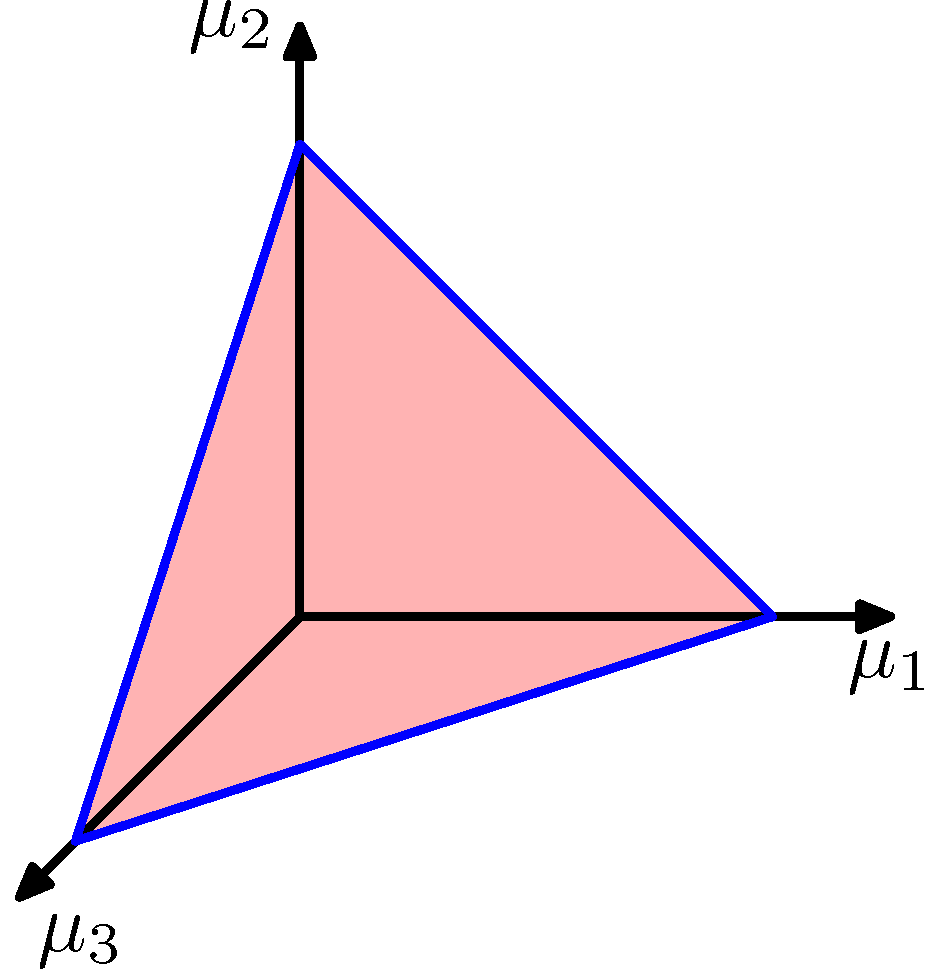
\includegraphics[scale=0.8]{Images/2-4.png}
		\captionsetup{font={small}}
		\caption{3个变量$\{\mu_1,\mu_2,\mu_3\}$的狄利克雷分布局限于如图所示的单型(即线性边界的流形)。这是限制条件$0 \leqslant \mu_k \leqslant 1$和$\sum_k\mu_k=1$所造成的。}
		\label{fig:2-4}
	\end{figure}
	\\
	\indent 该分布的归一化形式为
	\begin{equation}
		\mathrm{Dir}(\bfMu|\boldsymbol{\alpha})=\frac{\Gamma(\alpha_0)}{\Gamma(\alpha_1)...\Gamma(\alpha_K)}\prod_{k=1}^K\mu_k^{\alpha_k - 1}
	\end{equation}
	这就是狄利克雷分布(Dirichlet distribution)。其中,$\Gamma(x)$为Gamma函数,定义于(1.141),同时有
	\begin{equation}
		\alpha_0 = \sum_{k=1}^K \alpha_k
	\end{equation}
	在参数$\alpha_k$取不同的值时,单型上的狄利克雷分布如图2.5所示。
	\begin{figure}[ht]
	\centering
		\begin{minipage}[t]{0.3\linewidth}
		\centering
		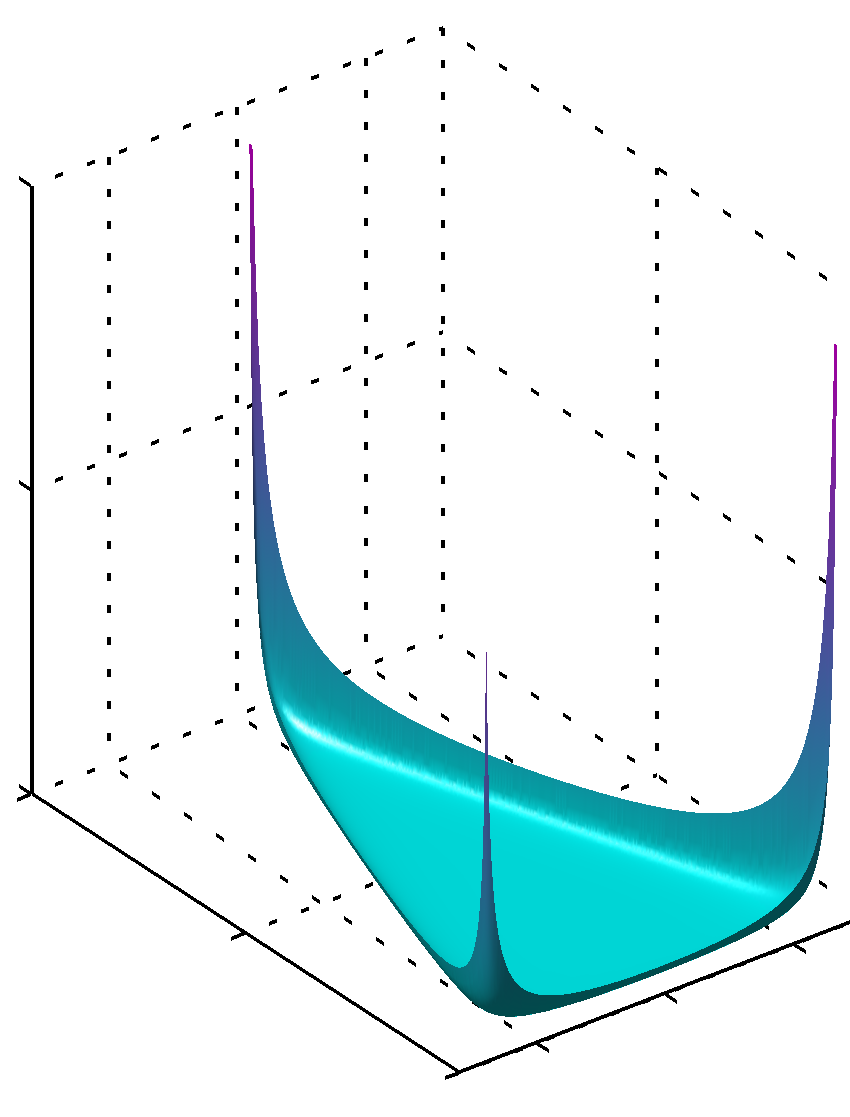
\includegraphics[scale=0.8]{Images/2-5a.png}
		\label{fig:2-5a}
		\end{minipage}
		\begin{minipage}[t]{0.3\linewidth}
		\centering
		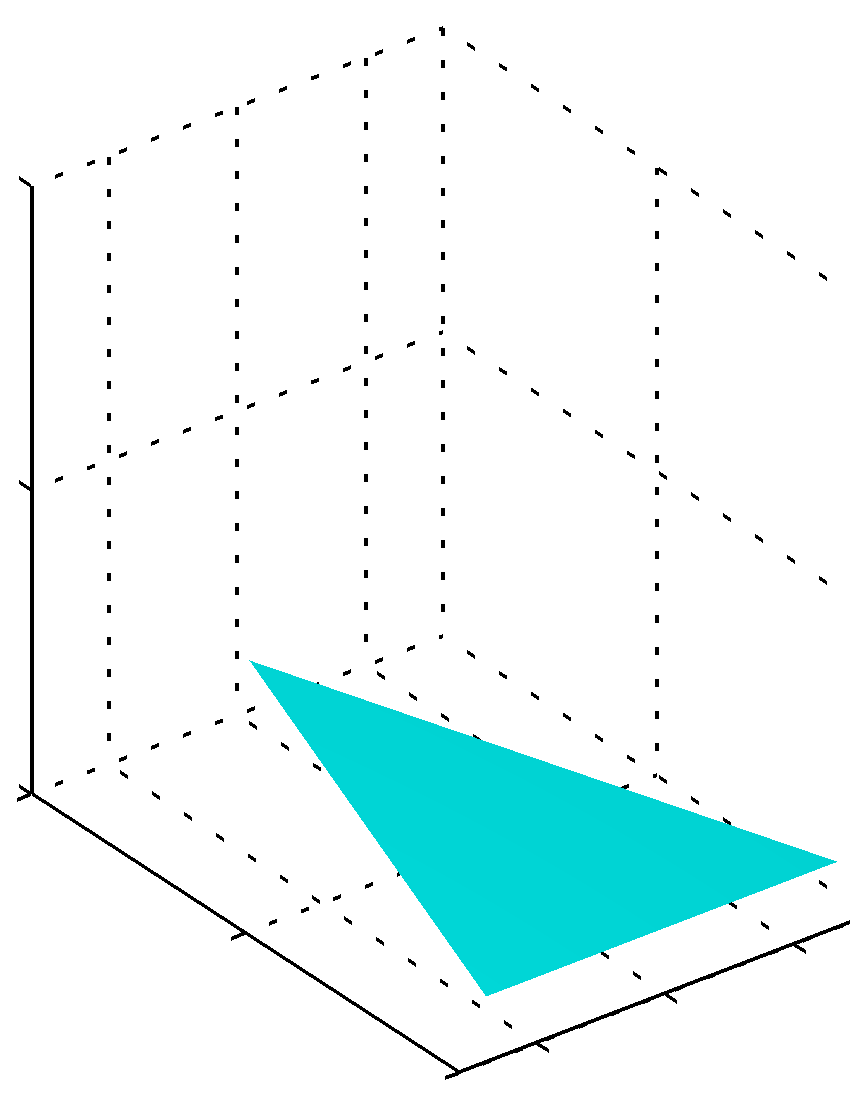
\includegraphics[scale=0.8]{Images/2-5b.png}
		\label{fig:2-5b}
		\end{minipage}
		\begin{minipage}[t]{0.3\linewidth}
		\centering
		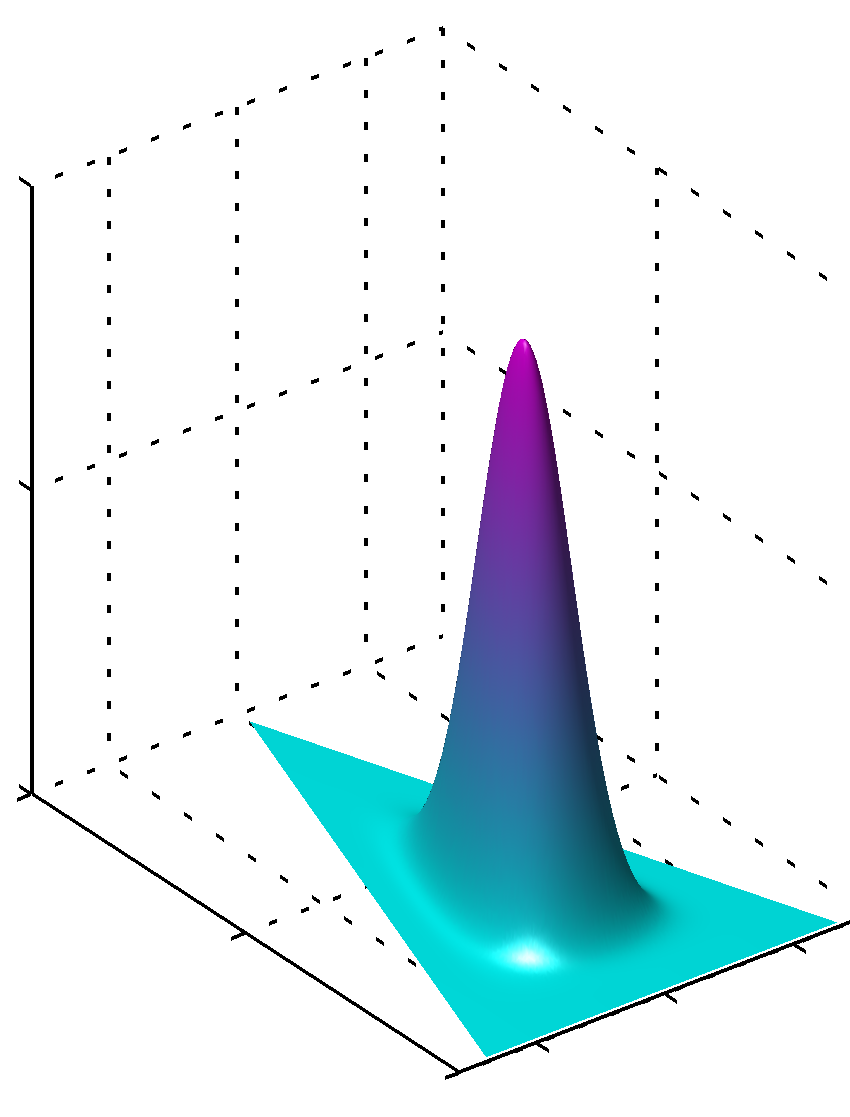
\includegraphics[scale=0.8]{Images/2-5c.png}
		\label{fig:2-5c}
		\end{minipage}
		\captionsetup{font={small}}
		\caption{3个变量的狄利克雷分布,其中两个水平轴是单型平面的坐标,垂直轴表示概率密度值。左图中$\{\alpha_k\}=0.1$,中间的图中$\{\alpha_k\}=1$,右图中$\{\alpha_k\}=10$。}
	\end{figure}
	\\
	\indent 将先验(2.38)乘以似然函数(2.34),我们可以得到参数$\{\mu_k\}$的后验分布
	\begin{equation}
		p(\bfMu|\mathcal{D},\boldsymbol{\alpha}) \propto p(\calD|\bfMu)p(\bfMu|\bfAl) \propto \prod_{k=1}^K \mu_k^{\alpha_k+m_k-1}
	\end{equation}
	可以看出后验分布也是狄利克雷分布的形式,也就确定了狄利克雷分布是多项分布的共轭先验。于是可以通过与(2.38)做一下对比来求取归一化常数
	\begin{equation}
	\begin{split}
		p(\bfMu|\calD,\bfAl) &= \mathrm{Dir}(\bfMu|\bfAl+\mathbf{m}) \\
		&=\frac{\Gamma(\alpha_0+N)}{\Gamma(\alpha_1+m_1)...\Gamma(\alpha_K+m_K)}\prod_{k=1}^K\mu_k^{\alpha_k+m_k-1}
	\end{split}
	\end{equation}
	其中$\mathbf{m}=(m_1,...,m_K)^{\rmT}$。正如beta分布之于二项分布,我们也可以将狄利克雷先验中的参数$\alpha_k$解释为$x_k=1$的有效数据量。\\
	\indent 需要注意的是,二值变量既可以表示为二元变量并利用二项分布(2.9)进行建模,也可以表示为 1-of-2 变量并利用多项分布(2.34)进行建模,在这种情况下,多项分布中的$K=2$。
	}
	\section{高斯分布}
	\insertline\\
	\textnormal{
	\indent 高斯分布,也就是正态分布,是连续变量中广泛使用的分布模型。对于一元变量$x$,高斯分布的形式为
	\begin{equation}
		\mathcal{N}(x|\mu,\sigma^2)=\frac{1}{(2\pi\sigma^2)^{1/2}}\exp\left\{-\frac{1}{2\sigma^2}(x-\mu)^2\right\}
	\end{equation}
	其中$\mu$为均值,$\sigma^2$为方差。对于$D$维向量$\bx$,多元高斯分布的形式为
	\begin{equation}
		\calN(\bx|\bfMu,\bfSigma)=\frac{1}{(2\pi)^{D/2}}\frac{1}{|\bfSigma|^{1/2}}\exp\left\{-\frac{1}{2}(\bx-\bfMu)^{\rmT}\bfSigma^{-1}(\bx-\bfMu)\right\}
	\end{equation}
	其中$D$维向量$\bfMu$为均值,$D \times D$矩阵$\bfSigma$为协方差矩阵,$|\bfSigma|$为$\bfSigma$的行列式。\\
	\indent 高斯分布具有广泛的应用,而且可以从很多不同的角度来解读。举例而言,我们已经看到对于一个一元实值变量,使得熵取得最大值的分布就是高斯分布。\textcolor{red}{\textbf{——第1.6节}}\ 这个性质同样适用于多元高斯分布。\textcolor{red}{\textbf{——习题 2.14}}\\
	\indent 另外,在研究多元随机变量的求和时我们也会用到高斯分布。根据中心极限定理,在不太严苛的条件下,随着求和项数量的增加,一组随机变量的总和(当然这本身就是一个随机变量)会越来越趋近于一个高斯分布(Walker, 1969)。假设有$N$个变量$x_1,...,x_N$,每个变量都服从$[0,1]$上的均匀分布,那么均值就是$(x_1+...+x_N)/N$。对于较大的$N$,如图2.6所示,这个分布会趋近于高斯分布。在实际应用中,随着$N$的增加,分布向高斯分布收敛的速度会非常快。一个比较典型的结果是,二项分布(2.9)将在$N \rightarrow \infty$时趋向于高斯分布,因为二项分布实际上是定义在$m$上的分布,而$m$表示的是二值变量$x$在$N$次观测中的结果总数(详见图2.1中$N=10$的情况)。
	\begin{figure}[ht]
	\centering
		\begin{minipage}[t]{0.3\linewidth}
		\centering
		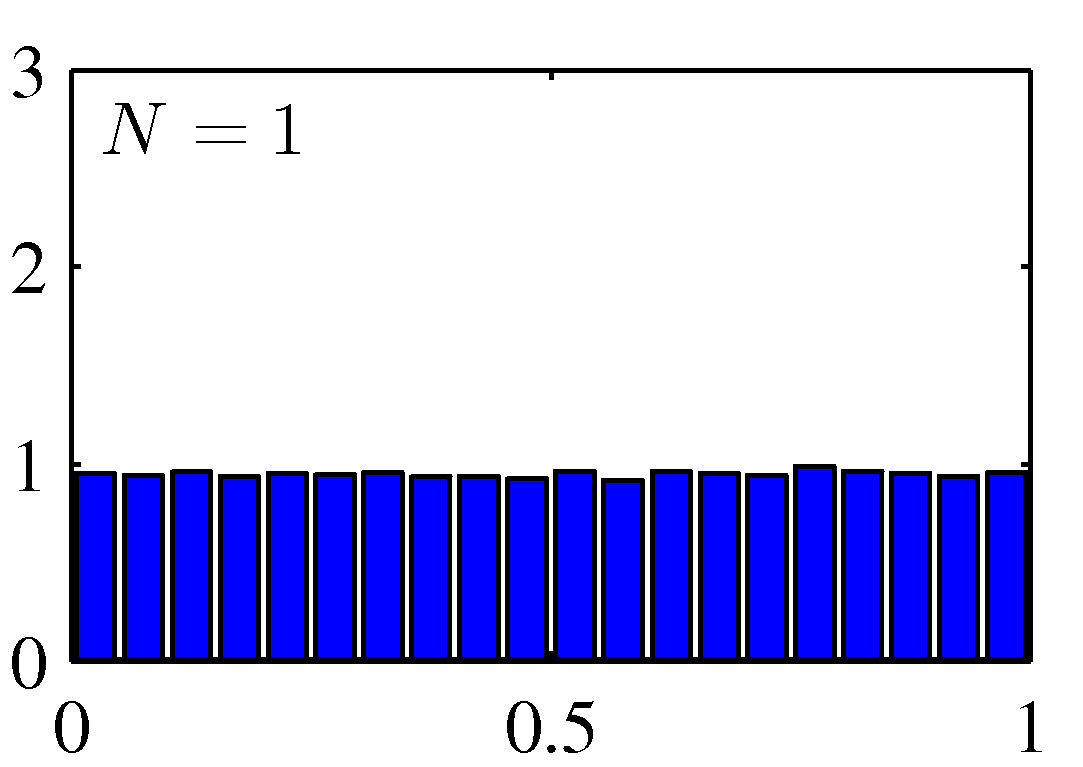
\includegraphics[scale=0.8]{Images/2-6a.png}
		\label{fig:2-6a}
		\end{minipage}
		\begin{minipage}[t]{0.3\linewidth}
		\centering
		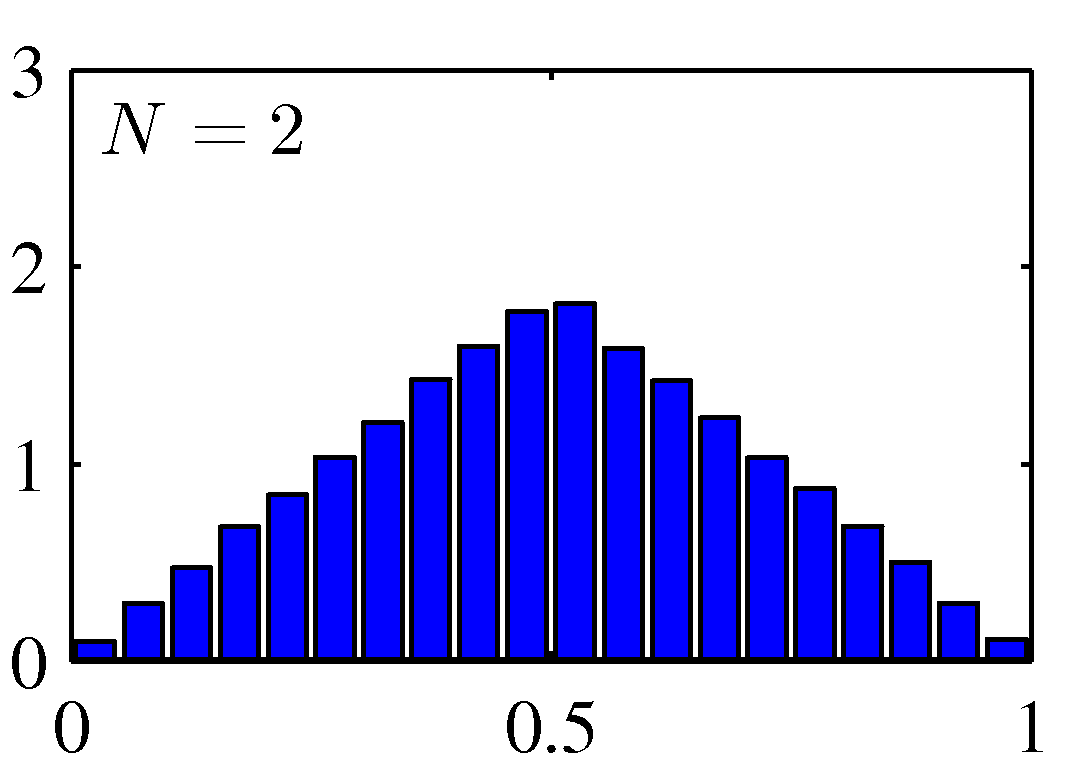
\includegraphics[scale=0.8]{Images/2-6b.png}
		\label{fig:2-6b}
		\end{minipage}
		\begin{minipage}[t]{0.3\linewidth}
		\centering
		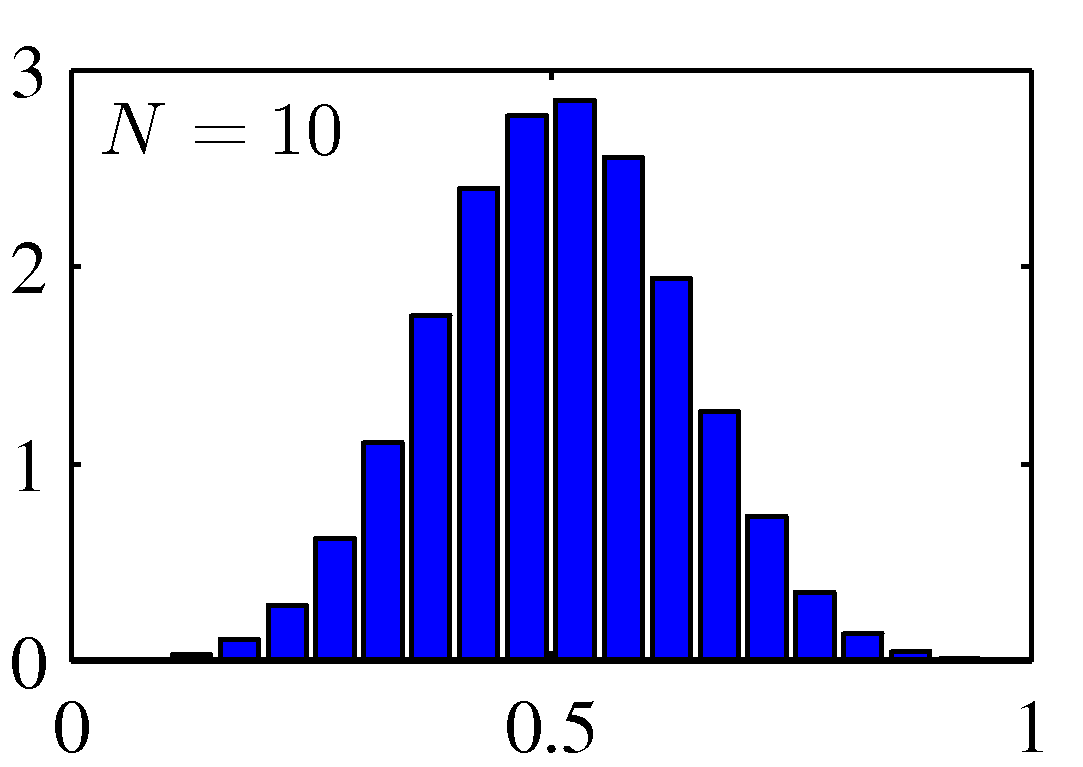
\includegraphics[scale=0.8]{Images/2-6c.png}
		\label{fig:2-6c}
		\end{minipage}
		\captionsetup{font={small}}
		\caption{当$N$取不同的值时,$N$个服从均匀分布的变量的均值直方图。可以看出随着$N$的增加,分布会趋近于高斯分布。}
	\end{figure}
	\\
	\indent 高斯分布具有很多重要的性质,我们很快就会详细地研究它们。于是乎,这一节会比前面的内容的技术含量更高,而且对矩阵的各种性质要求会比较高。\textcolor{red}{\textbf{——附录 C}}\ 尽管如此,我们还是强烈建议读者熟练掌握这一部分的内容,熟练操作高斯分布将会对后面章节中的复杂模型具有很大的帮助。请务必咬紧牙关,坚持下去。\\
	\indent 我们从高斯分布的几何形式开始。高斯分布中与$\bx$有关的部分是一个二次型
	\begin{equation}
		\Delta^2=(\bx-\bfMu)^{\rmT}\bfSigma^{-1}(\bx-\bfMu)
	\end{equation}
	这个二次型是出现在指数中的。$\Delta$表示的是$\bfMu$与$\bx$之间的马哈拉努比斯距离(即马氏距离,Mahalanobis distance,在后文中统一称为Mahalanobis距离),这个值将在$\bfSigma$为单位矩阵时退化为欧几里得距离。如果这个二次型为常数,那么这个高斯分布就是$\bx$空间中某个平面上的常数。\\
	\indent 首先,需要注意到矩阵$\bfSigma$一般可以认为是对称的,因为任何反对称分量都会在指数中消失。\textcolor{red}{\textbf{——习题 2.17} \ }对于协方差矩阵的特征向量方程
	\begin{equation}
		\bfSigma \mathbf{u}_i = \lambda_i \mathbf{u}_i
	\end{equation}
	其中$i=1,...,D$,由于$\bfSigma$是一个实对称矩阵,那么它的特征值一定是实数,其互异特征值对应的特征向量一定相互正交,\textcolor{red}{\textbf{——习题 2.18} \ }那么
	\begin{equation}
		\mathbf{u}_i^{\rmT} \mathbf{u}_j = I_{ij}
	\end{equation}
	其中$I_{ij}$为单位矩阵中的$\{i,j\}$元素,即
	\begin{equation}
		I_{ij}=\begin{cases}
		1,&\text{if}\ i=j \\
		0,&\text{otherwise}
		\end{cases}
	\end{equation}
	协方差矩阵可以表示为自身特征向量求和的形式\textcolor{red}{\textbf{——习题 2.19} \ }
	\begin{equation}
		\bfSigma=\sum_{i=1}^D\lambda_i\mathbf{u}_i\mathbf{u}_i^{\rmT}
	\end{equation}
	于是其逆矩阵$\bfSigma^{-1}$为
	\begin{equation}
		\bfSigma^{-1}=\sum_{i=1}^D\frac{1}{\lambda_i}\mathbf{u}_i\mathbf{u}_i^{\rmT}
	\end{equation}
	将(2.49)代入(2.44),二次型就变成了
	\begin{equation}
		\Delta^2=\sum_{i=1}^D\frac{y_i^2}{\lambda_i}
	\end{equation}
	其中
	\begin{equation}
		y_i=\mathbf{u}_i^{\rmT}(\bx - \bfMu)
	\end{equation}
	我们可以将$\{y_i\}$看成是正交向量$\mathbf{u}_i$下的新坐标系,当然,它是从原始的$x_i$坐标通过平移旋转得到的。构建向量$\mathbf{y}=(y_1,...,y_D)^{\rmT}$,可得
	\begin{equation}
		\mathbf{y}=\mathbf{U}(\mathbf{x}-\bfMu)
	\end{equation}
	其中的$\mathbf{U}$是以$\mathbf{u}_i^{\rmT}$为行的矩阵。根据(2.46),$\mathbf{U}$为正交矩阵,即$\mathbf{U}\mathbf{U}^{\rmT}=\mathbf{I}$,同时$\mathbf{U}^{\rmT}\mathbf{U}=\mathbf{I}$,其中$\mathbf{I}$为单位矩阵。\textcolor{red}{\textbf{——附录 C} \ }\\
	\indent 当(2.50)为常数时,该二次型将是某平面上的常数,则高斯概率密度也是常数。如果所有的特征值$\lambda_i$均为正数,该平面就是椭球面,其中心为$\bfMu$,轴的方向为$\mathbf{u}_i$,轴长的缩放因子为$\lambda_i^{1/2}$,如图2.7所示。
	\begin{figure}[ht]
		\centering
		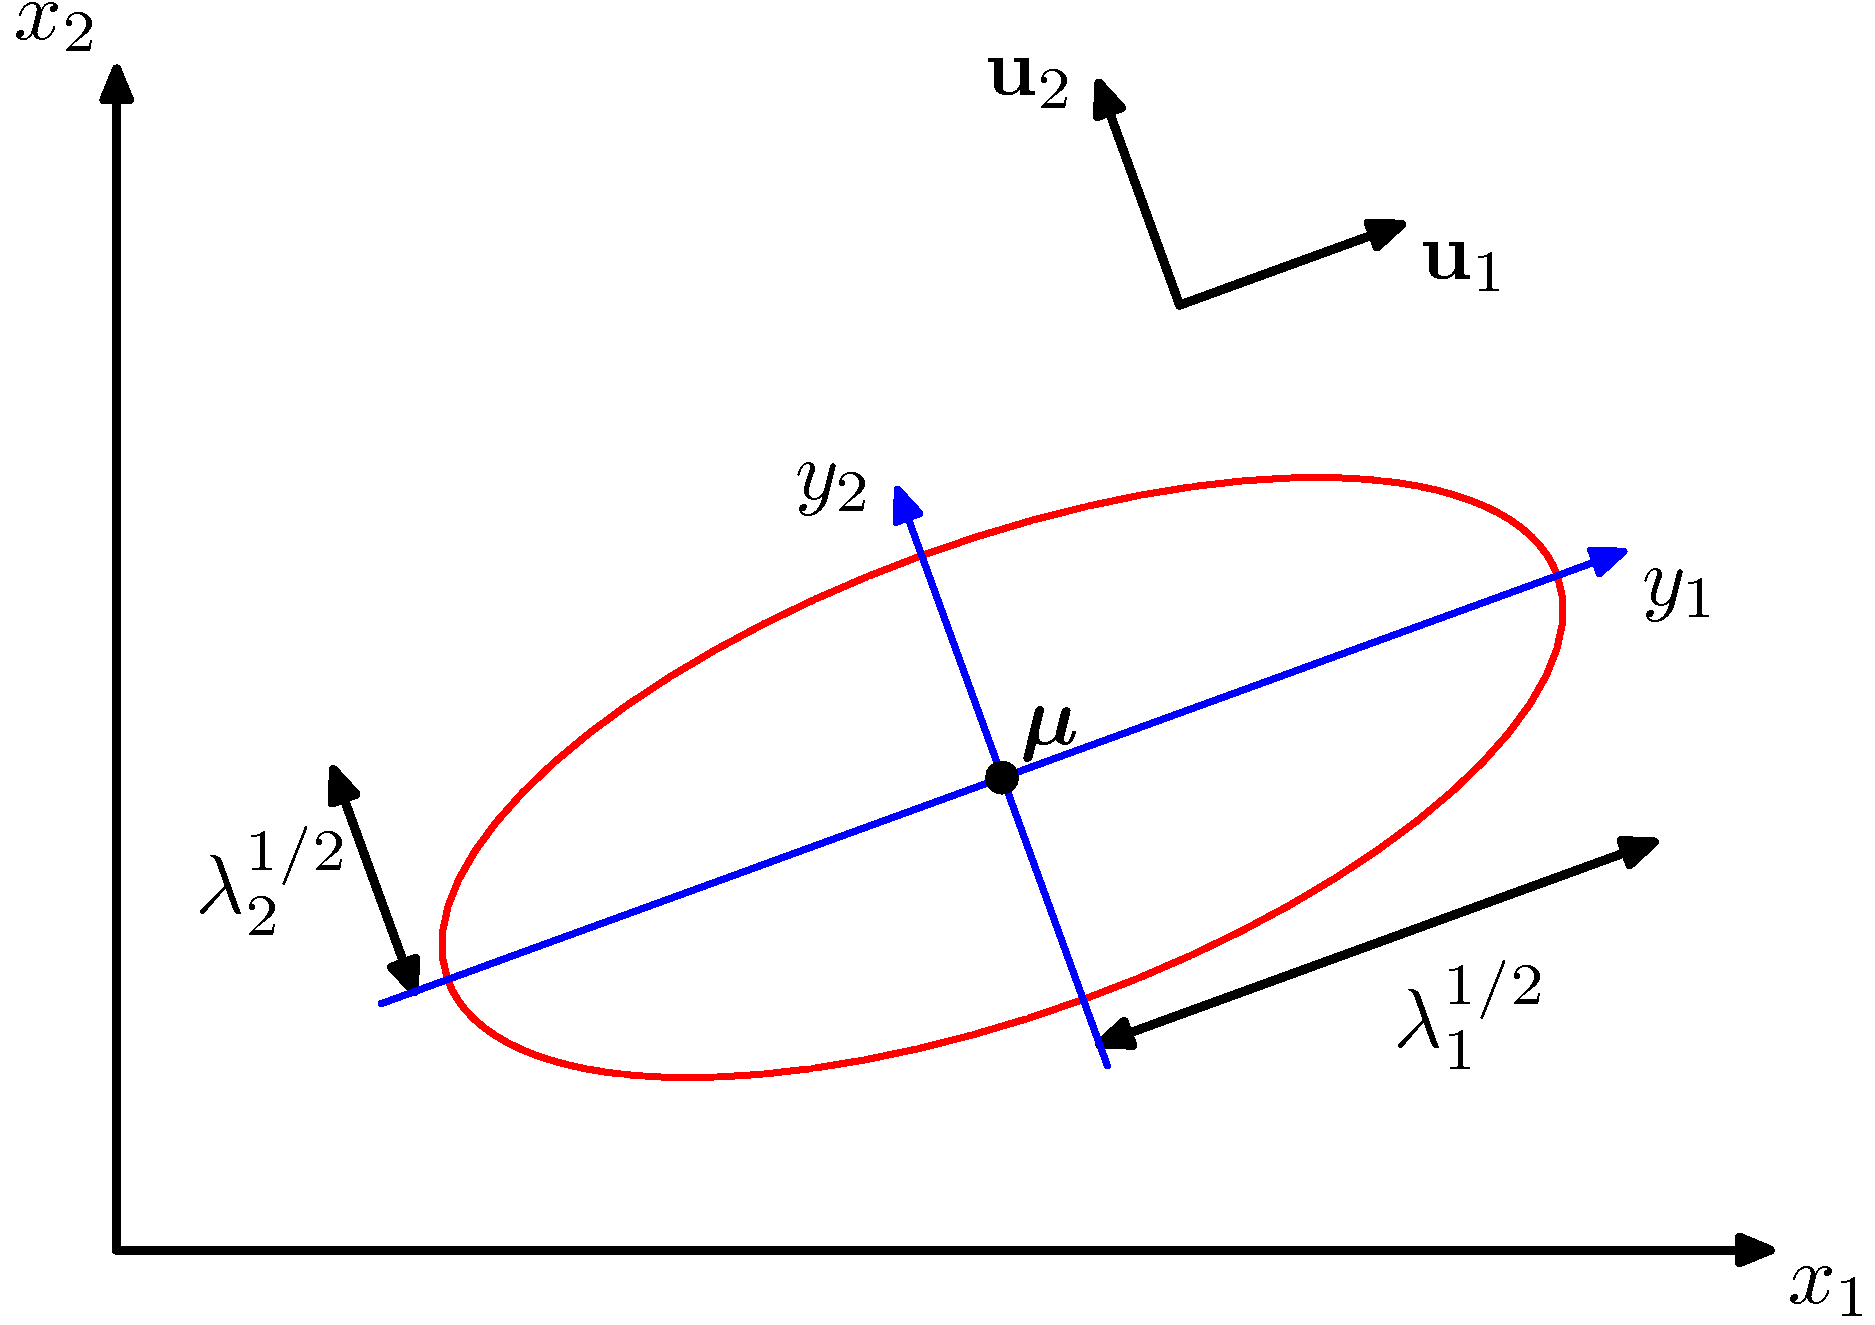
\includegraphics[scale=0.8]{Images/2-7.png}
		\captionsetup{font={small}}
		\caption{图中红色的曲线表示的是二维空间$\bx=(x_1,x_2)$的常数概率分布椭球面,对应的是$\bx=\bfMu$处的概率密度为$\exp{-1/2}$。椭圆的两条轴是由协方差矩阵的特征向量$\mathbf{u}_i$得到的,其对应的特征值为$\lambda_i$。}
		\label{fig:2-7}
	\end{figure}
	\\
	\indent 高斯分布要求其协方差矩阵的特征值$\lambda_i$严格为正数,否则分布就不能归一化。特征值严格为正的矩阵称为正定矩阵。在第12章中,我们会遇到具有0特征值的高斯分布,这种情况下的分布是奇异的,而且被限制在了低维的子空间中。如果所有的特征值都是非负的,那么协方差矩阵就是半正定矩阵。\\
	\indent 现在我们来研究新坐标$y_i$下的高斯分布。在$\bx$变换成$\mathbf{y}$的过程中,有雅可比矩阵$\mathbf{J}$:
	\begin{equation}
		J_{ij}=\frac{\partial x_i}{\partial y_i}=U_{ji}
	\end{equation}
	其中的$U_{ji}$为矩阵$\mathbf{U}^{\rmT}$的元素。根据矩阵$\mathbf{U}$的对称性,可以看出雅可比矩阵行列式的平方为
	\begin{equation}
		|\mathbf{J}|^2 = |\mathbf{U}^{\rmT}|^2 = |\mathbf{U}^{\rmT}||\mathbf{U}|=|\mathbf{U}^{\rmT}\mathbf{U}|=|\mathbf{I}|=1
	\end{equation}
	于是$|\mathbf{J}|=1$,而且协方差矩阵的行列式$|\bfSigma|$可以写成特征值乘积的形式:
	\begin{equation}
		|\bfSigma|^{1/2}=\prod_{j=1}^D\lambda_j^{1/2}
	\end{equation}
	于是在$y_i$坐标系中,高斯分布的形式为
	\begin{equation}
		p(\mathbf{y})=p(\mathbf{x})|\mathbf{J}| = \prod_{j=1}^D\frac{1}{(2\pi\lambda_j)^{1/2}}\exp\left\{-\frac{y_j^2}{2\lambda_j}\right\}
	\end{equation}
	事实上就是$D$个相互独立的一元高斯分布的乘积。于是特征向量定义了一个经过平移和旋转的新坐标系,在这个坐标系中,联合概率分布可以分解为若干独立分布的乘积。在$\mathbf{y}$坐标系中的积分为
	\begin{equation}
		\int p(\mathbf{y})\ \mathrm{d}\mathbf{y} = \prod_{j=1}^D\int_{-\infty}^{\infty}\frac{1}{(2\pi\lambda_j)^{1/2}}\exp \left\{-\frac{y_j^2}{2\lambda_j}\right\}\ \mathrm{d}y_i=1
	\end{equation}
	其中我们利用了(1.48)中一元高斯函数归一化的结论。这也验证了多元高斯分布(2.43)确实是归一化的。\\
	\indent 我们现在来研究一下高斯分布的矩,从而解释一下参数$\bfMu$和$\bfSigma$的含义。在高斯分布下$\bx$的期望为
	\begin{equation}
	\begin{split}
		\mathbb{E}[\bx] &= \frac{1}{(2\pi)^{D/2}} \frac{1}{|\bfSigma|^{1/2}}\int \exp \left\{-\frac{1}{2}(\bx-\bfMu)^{\rmT}\bfSigma^{-1}(\bx-\bfMu)\right\}\bx \ \mathrm{d}\bx \\
		&=\frac{1}{(2\pi)^{D/2}} \frac{1}{|\bfSigma|^{1/2}}\int \exp \left\{-\frac{1}{2}\mathbf{z}^{\rmT}\bfSigma^{-1}\mathbf{z}\right\}(\mathbf{z}+\bfMu) \ \mathrm{d}\mathbf{z}
	\end{split}
	\end{equation}
	其中进行了变量的替换$\mathbf{z}=\bx-\bfMu$。此时注意到积分号里的指数部分是关于$\mathbf{z}$的偶函数,而积分区间是$(-\infty,\infty)$,很明显是对称区间,而带上$(\mathbf{z}+\bfMu)$中$\mathbf{z}$的那一项变成了奇函数,于是在积分之后就消失了,再利用一下高斯分布的归一化条件,最后的结果为
	\begin{equation}
		\mathbb{E}[\bx]=\bfMu
	\end{equation}
	所以$\bfMu$就是高斯分布的均值。\\
	\indent 下面研究高斯分布的二阶矩。在一元变量的情况下,要计算的二阶矩为$\mathbb{E}[x^2]$;而对于多元高斯分布,二阶矩有$D^2$个,分别由$\mathbb{E}[x_i x_j]$给出,可以写成矩阵的形式$\mathbb{E}[\bx\bx^{\rmT}]$。这个矩阵实际上就是
	\[
	\begin{split}
		\mathbb{E}[\bx\bx^{\rmT}]&=\frac{1}{(2\pi)^{D/2}}\frac{1}{|\bfSigma|^{1/2}}\int \exp\left\{-\frac{1}{2}(\bx-\bfMu)^{\rmT}\bfSigma^{-1}(\bx-\bfMu)\right\}\bx \bx^{\rmT}\ \mathrm{d}\bx \\
		&=\frac{1}{(2\pi)^{D/2}}\frac{1}{|\bfSigma|^{1/2}}\int \exp\left\{-\frac{1}{2}\mathbf{z}^{\rmT}\bfSigma^{-1}\mathbf{z}\right\}(\mathbf{z}+\bfMu) (\mathbf{z}+\bfMu)^{\rmT}\ \mathrm{d}\mathbf{z}
	\end{split}
	\]
	其中再次用到了变量替换$\mathbf{z}=\bx-\bfMu$。需要注意的是,交叉项$\bfMu\mathbf{z}^{\rmT}$和$\mathbf{z}\bfMu^{\rmT}$会由于对称性而消失。$\bfMu\bfMu^{\rmT}$为常数,所以可以提到积分号外面,由于高斯分布是归一化的,所以它是一个单位矩阵。对于包含有$\mathbf{z}\mathbf{z}^{\rmT}$的那一项,再次根据(2.45)对协方差矩阵利用其互异的特征向量进行展开,于是有
	\begin{equation}
		\mathbf{z}=\sum_{j=1}^Dy_j\mathbf{u}_j
	\end{equation}
	其中$y_j=\mathbf{u}_j^{\rmT}\mathbf{z}$,于是有
	\begin{equation}
	\begin{split}
		&\frac{1}{(2\pi)^{D/2}}\frac{1}{|\bfSigma|^{1/2}}\int \exp \left\{-\frac{1}{2}\mathbf{z}^{\rmT}\bfSigma^{-1}\mathbf{z}\right\}\mathbf{z}\mathbf{z}^{\rmT}\ \mathrm{d}\mathbf{z}\\
		= &\frac{1}{(2\pi)^{D/2}}\frac{1}{|\bfSigma|^{1/2}}\sum_{i=1}^D \sum_{j=1}^D \mathbf{u}_i\mathbf{u}_j^{\rmT}\int \exp\left\{-\sum_{k=1}^D \frac{y_k^2}{2\lambda_k}\right\}y_iy_j\ \mathrm{d}\mathbf{y}\\
		= &\sum_{i=1}^D\mathbf{u}_i\mathbf{u}_i^{\rmT}\lambda_i = \bfSigma
	\end{split}
	\end{equation}
	其中使用了特征向量方程(2.45),并利用了一条性质:等号右侧的积分中,根据对称性,除非$i=j$,否则全部为0。最后一行的计算我们利用了结论(1.50)和(2.55),以及(2.48)。于是就有
	\begin{equation}
		\mathbb{E}[\bx\bx^{\rmT}]=\bfMu\bfMu^{\rmT}+\bfSigma
	\end{equation}
	\indent 对于一元随机变量,我们在定义方差之前要减去均值。类似地,对于多元变量的情况,我们也要减掉均值,从而得到随机变量$\bx$的协方差:
	\begin{equation}
		\mathrm{cov}[\bx]=\mathbb{E}\left[(\bx-\mathbb{E}[\bx])(\bx-\mathbb{E}[\bx]^{\rmT})\right]
	\end{equation}
	对于高斯分布,我们将$\mathbb{E}[\bx]=\bfMu$和(2.62)一同代入,得到
	\begin{equation}
		\mathrm{cov}[\bx]=\bfSigma
	\end{equation}
	由于参数$\bfSigma$控制了高斯分布下$\bx$的协方差,所以被称为协方差矩阵。\\
	\indent 尽管高斯分布(2.43)是广泛应用的概率密度模型,但它也具有很多明显的局限性。分布中自由参数的数量就是个问题,随便一个对称的协方差矩阵$\bfSigma$就有$D(D+1)/2$个独立参数,另外在$\bfMu$中还有另外$D$个,加起来足足有$D(D+3)/2$个独立参数。对于较大的$D$,独立参数的数量会随着$D$的增加呈平方型增长,求这样的大矩阵的乘积和逆,计算压力相当大,甚至可能是无解的。解决这个问题的方法之一,是限制协方差矩阵的形式。对于协方差矩阵为对角阵的情况,$\bfSigma=\mathrm{diag}(\sigma_i^2)$,于是概率密度模型中独立参数的数量为$2D$。其对应的常数概率密度的轮廓线为轴对称的椭球面。要是更严格一些,我们可以限制协方差矩阵为常数与单位矩阵的乘积,即$\bfSigma=\sigma^2 \mathbf{I}$,也就是协方差各向同性(isotropic),这样的话模型中独立参数的数量为$D+1$,椭球面也就变成了球面。一般、对角和各项同性三种协方差矩阵对应的概率密度如图2.8所示。不幸的是,尽管我们通过这样的方法限制了分布的自由度,使得协方差矩阵的逆求起来更加方便和快捷,但这样的做法也严重限制了概率密度的形式,同时也限制了模型抓住数据中最有用内容的能力。
	\begin{figure}[ht]
	\centering
		\begin{minipage}[t]{0.3\linewidth}
		\centering
		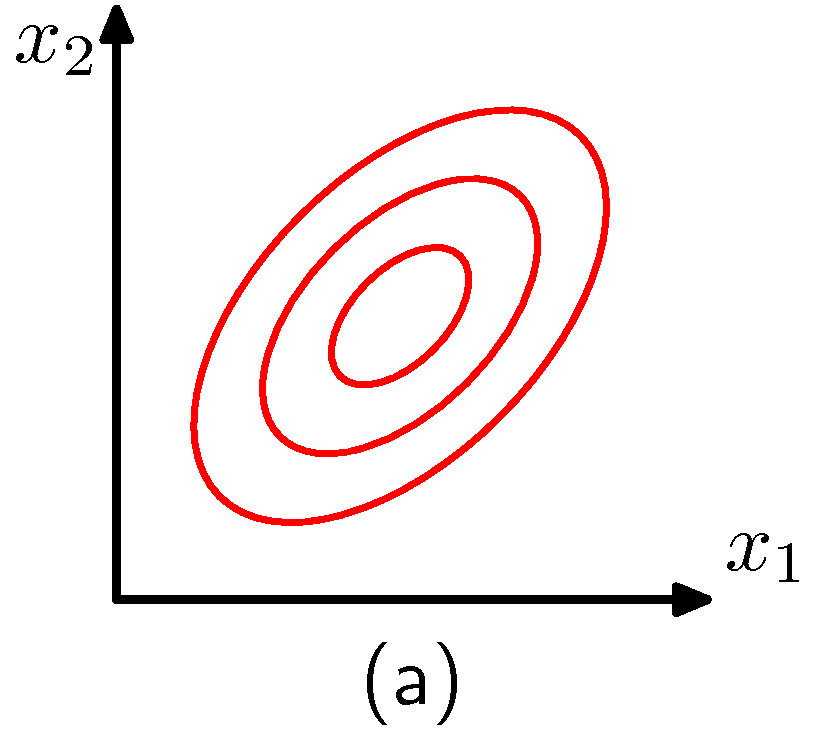
\includegraphics[scale=0.8]{Images/2-8a.png}
		\label{fig:2-8a}
		\end{minipage}
		\begin{minipage}[t]{0.3\linewidth}
		\centering
		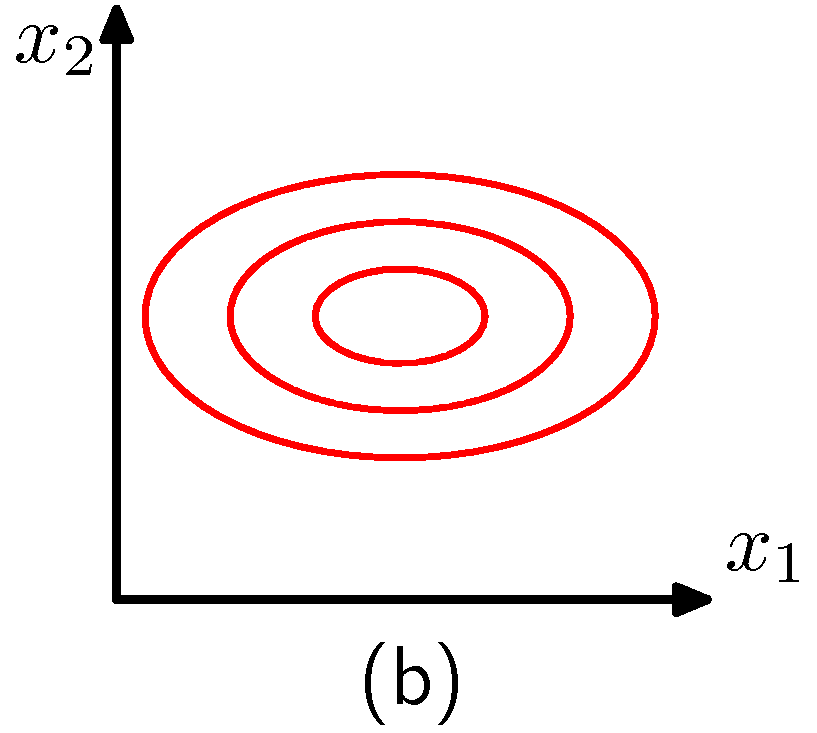
\includegraphics[scale=0.8]{Images/2-8b.png}
		\label{fig:2-8b}
		\end{minipage}
		\begin{minipage}[t]{0.3\linewidth}
		\centering
		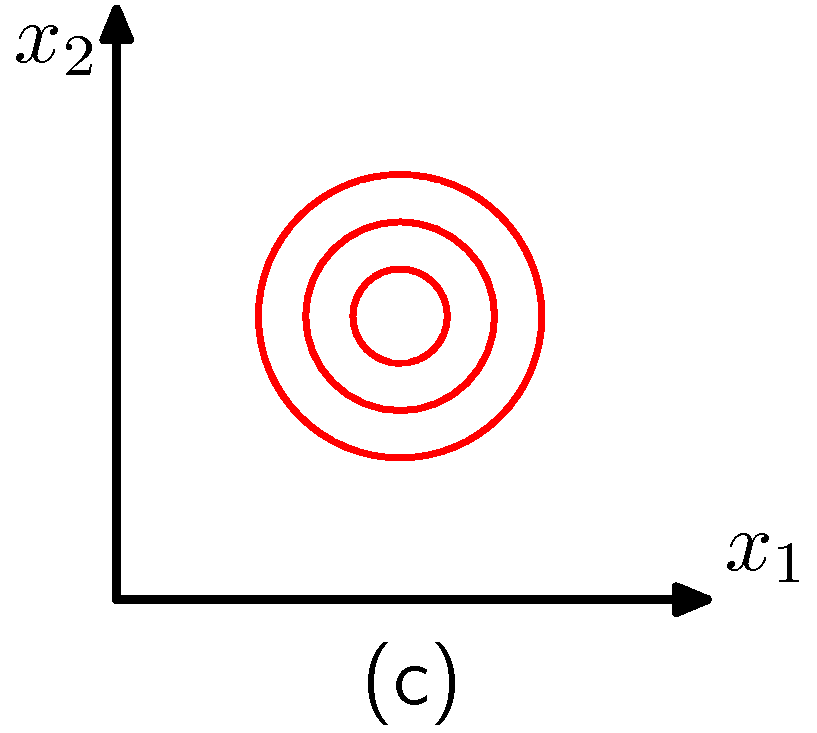
\includegraphics[scale=0.8]{Images/2-8c.png}
		\label{fig:2-8c}
		\end{minipage}
		\captionsetup{font={small}}
		\caption{二维高斯分布的常数概率密度轮廓线,(a)为一般情况;(b)为协方差矩阵为对角矩阵的情况,图中椭圆的两轴分别与两个坐标轴平行;(c)为协方差矩阵与单位矩阵成比例的情况,前几个图中的椭圆变成了圆。}
	\end{figure}
	\\
	\indent 高斯分布的另一个重要限制是,这个分布是单峰的——也就是只有一个最大值。于是高斯分布对于多峰分布的拟合自然显得力不从心。所以,作为一个带有很多参数的分布,高斯分布很灵活,但又有可能因为自身能够有效拟合的分布太少,而在应用中受到严重的限制。我们会在后文中介绍隐变量(latent variables)时解决以上的两个问题。特别地,如果将离散隐变量放到高斯混合模型中,将会得到一个很大的多峰分布族,我们将在第2.3.9节中介绍这个内容。类似地,在第12章中即将介绍的连续隐变量将使我们可以得到自由参数的数量可以由数据空间的维数$D$独立控制,又可以获取数据集里的核心内容的模型。实际上,这两个方法是可以联合在一起的,可以通过它们得到种类繁多的分层模型,在实际应用中可以广泛使用。举例而言,马尔科夫随机场(Markov random field)的高斯形态广泛应用于图像的概率模型中。它其实是一个像素空间中的高斯分布,但引入了能够反映像素空间组织结构的内容,从而处理起来更加方便。类似地,线性动态系统(linear dynamical system)可以用于时序数据的建模,比如说追踪,其实线性动态系统同样是建立在大量观测变量和隐变量上的联合高斯分布,所以同样可以得到有效的应对。为了表示这些复杂分布的形式和属性,我们会用到一种强大的框架——概率图模型,相关内容将在第8章中进行介绍。
	}
	\subsection{条件高斯分布}
	\textnormal{
	多元高斯分布具有一个很重要的性质,如果两组变量服从联合高斯分布,那么给定其中一组的条件下另一组的条件分布同样也是高斯分布,而且对两组变量的任意一组求边缘分布,得到的分布同样也是高斯分布。\\
	\indent 首先研究一下条件分布的情况。假设$\bx$是一个$D$维向量,服从高斯分布$\mathcal{N}(\bx|\bfMu,\bfSigma)$。现在将$\bx$拆分成两个相互独立的子集$\bx_a$和$\bx_b$,一般地,我们可以将$\bx_a$设置为$\bx$的前$M$个分量,而$\bx_b$则是$\bx$的后$D-M$个分量。于是
	\begin{equation}
		\bx = \left(\begin{matrix}\bx_a \\ \bx_b \end{matrix}\right)
	\end{equation}
	同样地将均值向量$\bfMu$对应拆开:
	\begin{equation}
		\bfMu = \left(\begin{matrix} \bfMu_a \\ \bfMu_b \end{matrix}\right)
	\end{equation}
	以及协方差矩阵:
	\begin{equation}
		\bfSigma=\left(\begin{matrix} \bfSigma_{aa} & \bfSigma_{ab} \\ \bfSigma_{ba} & \bfSigma_{bb} \end{matrix}\right)
	\end{equation}
	根据协方差矩阵的对称性$\bfSigma^{\rmT}=\bfSigma$,$\bfSigma_{aa}$和$\bfSigma_{bb}$都是对称矩阵,以及$\bfSigma_{ba}=\bfSigma_{ab}^{\rmT}$。\\
	\indent 在很多情况下,利用协方差矩阵的逆矩阵会更方便一些:
	\begin{equation}
		\boldsymbol{\Lambda} \equiv \bfSigma^{-1}
	\end{equation}
	这就是精度矩阵(precision matrix)。实际上,高斯分布的一些性质用协方差矩阵表示会比较方便,但还有很多性质用精度矩阵表示会更加方便。于是再多关注一下精度矩阵的拆分形式:
	\begin{equation}
		\boldsymbol{\Lambda}=\left(\begin{matrix}\boldsymbol{\Lambda}_{aa} & \boldsymbol{\Lambda}_{ab} \\ \boldsymbol{\Lambda}_{ba} & \boldsymbol{\Lambda}_{bb}\end{matrix}\right)
	\end{equation}
	拆分的形式也是对应着(2.65)中$\bx$的拆分形式的。由于对称矩阵的逆矩阵仍然是对称矩阵,\textcolor{red}{\textbf{——习题 2.22\ }}可以看出$\boldsymbol{\Lambda}_{aa}$和$\boldsymbol{\Lambda}_{bb}$为对称矩阵,以及$\boldsymbol{\Lambda}_{ab}^{\rmT}=\boldsymbol{\Lambda}_{ba}$。不过这里需要指出一个问题,$\bfLambda_{aa}$绝不仅仅是$\bfSigma_{aa}$求逆那么简单。我们现在就来研究一下分块矩阵的逆矩阵及其分块的逆矩阵。\\
	\indent 就从求取条件分布$p(\bx_a|\bx_b)$的表达式开始。根据概率的乘法规则,这个条件分布可以根据联合分布$p(\bx)=p(\bx_a,\bx_b)$求出,只需要将$\bx_b$设为固定值并进行归一化,最后就可以得到给定$\bx_b$的条件下$\bx_a$的概率分布。不过,与其按部就班地计算,我们不如先利用一下高斯分布中指数项里的二次型(2.44)的特殊性,然后再做归一化,这样可以更快地得到结果。根据(2.65)、(2.66)和(2.69)中的分块,可以得到
	\begin{equation}
	\begin{split}
		-\frac{1}{2}&(\bx-\bfMu)^{\rmT}\bfSigma^{-1}(\bx-\bfMu) = \\
		&-\frac{1}{2}(\bx_a-\bfMu_a)^{\rmT}\bfLambda_{aa}(\bx_a-\bfMu_a)-\frac{1}{2}(\bx_a-\bfMu_a)^{\rmT}\bfLambda_{ab}(\bx_b-\bfMu_b) \\ &-\frac{1}{2}(\bx_b-\bfMu_b)^{\rmT}\bfLambda_{ba}(\bx_a-\bfMu_a)-\frac{1}{2}(\bx_b-\bfMu_b)^{\rmT}\bfLambda_{bb}(\bx_b-\bfMu_b)
	\end{split}
	\end{equation}
	可以看出这是一个关于$\bx_a$的函数,而且同样是一个二次型,于是对应的条件分布$p(\bx_a|\bx_b)$也是一个高斯分布。由于这个分布完全由其均值和协方差确定,于是我们只需要根据(2.70)确定$p(\bx_a|\bx_b)$的均值和方差就可以确定整个分布了。\\
	\indent 对于高斯分布,“完成平方项”是一个相当常见的操作。在给定了高斯分布指数项中的二次型后,据此确定分布的均值和方差。这个问题可以这样解决,首先注意到高斯分布$\mathcal{N}(\bx|\bfMu,\bfSigma)$可以写成
	\begin{equation}
		-\frac{1}{2}(\bx-\bfMu)^{\rmT}\bfSigma^{-1}(\bx-\bfMu)=-\frac{1}{2}\bx^{\rmT}\bfSigma^{-1}\bx + \bx^{\rmT}\bfSigma^{-1}\bfMu + \mathrm{const}
	\end{equation}
	其中“const”表示的是与$\bx$无关的项,并利用了$\bfSigma$的对称性。所以对于一个一般的二次型,如果我们将它拆分成(2.71)的形式,那么就可以令$\bx$二次项的系数矩阵为协方差矩阵的逆矩阵$\bfSigma^{-1}$,令$\bx$一次项的系数向量为$\bfSigma^{-1}\bfMu$,于是就可以确定$\bfMu$了。\\
	\indent 现在我们用这个方法求取条件高斯分布$p(\bx_a|\bx_b)$,其指数项中的二次型就是(2.70)。我们用$\bfMu_{a|b}$表示均值,$\bfSigma_{a|b}$表示方差,将(2.70)看作是$\bx_a$的函数,将$\bx_b$看作是常数,对于$\bx_a$的二次项,其形式为
	\begin{equation}
		-\frac{1}{2}\bx_a^{\rmT}\bfLambda_{aa}\bx_a
	\end{equation}
	于是马上得到$p(\bx_a|\bx_b)$的协方差矩阵为
	\begin{equation}
		\bfSigma_{a|b}=\bfLambda_{aa}^{-1}
	\end{equation}
	对于(2.70)中$\bx_a$的一次项,
	\begin{equation}
		\bx_a^{\rmT}\{\bfLambda_{aa}\bfMu_a - \bfLambda_{ab}(\bx_b-\bfMu_b)\}
	\end{equation}
	其中用到了$\bfLambda_{ba}^{\rmT}=\bfLambda_{ab}$。根据(2.71),这个表达式中$\bx_a$的系数一定等于$\bfSigma_{a|b}^{-1}\bfMu_{a|b}$,于是根据(2.73),
	\begin{equation}
	\begin{split}
		\bfMu_{a|b} &= \bfSigma_{a|b}\{\bfLambda_{aa}\bfMu_a-\bfLambda_{ab}(\bx_b-\bfMu_b)\} \\
		&= \bfMu_a-\bfLambda_{aa}^{-1}\bfLambda_{ab}(\bx_b-\bfMu_b)
	\end{split}
	\end{equation}
	\indent (2.73)和(2.75)是根据原始的联合分布$p(\bx_a,\bx_b)$的精度矩阵的分块形式确定的,我们也可以对协方差矩阵进行分块得到这样的结果。为了完成这一点,我们利用如下的分块矩阵的逆矩阵的恒等式:
	\begin{equation}
		\left(\begin{matrix}\mathbf{A} & \mathbf{B} \\ \mathbf{C} & \mathbf{D} \end{matrix}\right)^{-1}=\left(\begin{matrix}\mathbf{M} & -\mathbf{MBD}^{-1} \\ -\mathbf{D}^{-1}\mathbf{CM} & \mathbf{D}^{-1}+\mathbf{D}^{-1}\mathbf{CMBD}^{-1}\end{matrix}\right)
	\end{equation}
	其中定义了
	\begin{equation}
		\mathbf{M}=(\mathbf{A}-\mathbf{BD}^{-1}\mathbf{C})^{-1}
	\end{equation}
	\textcolor{red}{\textbf{译者注:所以完整的矩阵为:}
	\[
		\left(\begin{matrix}\mathbf{A} & \mathbf{B} \\ \mathbf{C} & \mathbf{D} \end{matrix}\right)^{-1}=\left(\begin{matrix}(\mathbf{A}-\mathbf{BD}^{-1}\mathbf{C})^{-1} & -\mathbf{MBD}^{-1} \\ -\mathbf{D}^{-1}\mathbf{C}(\mathbf{A}-\mathbf{BD}^{-1}\mathbf{C})^{-1} & \mathbf{D}^{-1}+\mathbf{D}^{-1}\mathbf{C}(\mathbf{A}-\mathbf{BD}^{-1}\mathbf{C})^{-1}\mathbf{BD}^{-1}\end{matrix}\right)
	\]}
	其中的$\mathbf{M}^{-1}$就是(2.76)等号左侧的矩阵关于矩阵块$\mathbf{D}$的舒尔补(Schur complement)。根据定义,
	\begin{equation}
		\left(\begin{matrix}\bfSigma_{aa} & \bfSigma_{ab} \\ \bfSigma_{ba} & \bfSigma_{bb}\end{matrix}\right)^{-1} = \left(\begin{matrix}\bfLambda_{aa} & \bfLambda_{ab} \\ \bfLambda_{ba} & \bfLambda_{bb}\end{matrix}\right)
	\end{equation}
	以及根据(2.76),可以得到
	\begin{align}
		\bfLambda_{aa}&=(\bfSigma_{aa}-\bfSigma_{ab}\bfSigma_{bb}^{-1}\bfSigma_{ba})^{-1}\\
		\bfLambda_{ab}&=-(\bfSigma_{aa}-\bfSigma_{ab}\bfSigma_{bb}^{-1}\bfSigma_{ba})^{-1}\bfSigma_{ab}\bfSigma_{bb}^{-1}
	\end{align}
	根据这些,我们可以确定条件分布$p(\bx_a|\bx_b)$的均值和协方差的表达式
	\begin{align}
		\bfMu_{a|b}&=\bfMu_a + \bfSigma_{ab}\bfSigma_{bb}^{-1}(\bx_b-\bfMu_b) \\
		\bfSigma_{a|b}&=\bfSigma_{aa}-\bfSigma_{ab}\bfSigma_{bb}^{-1}\bfSigma_{ba}
	\end{align}
	通过对比(2.73)和(2.82),可以看出用精度矩阵表示条件分布$p(\bx_a|\bx_b)$比协方差矩阵更加简单。需要注意的是,(2.81)中条件分布$p(\bx_a|\bx_b)$的均值是关于$\bx_b$的线性函数,(2.82)中给出的协方差与$\bx_b$无关。这是线性高斯模型(linear-Gaussian model)的典型案例之一。\textcolor{red}{\textbf{——第8.1.4节}}
	}
	\subsection{边缘高斯分布}
	\textnormal{
	我们已经看到,如果联合分布$p(\bx_a, \bx_b)$为高斯分布,那么条件分布$p(\bx_a|\bx_b)$一定也是一个高斯分布。现在我们转向边缘分布的讨论,也就是
	\begin{equation}
		p(\bx_a)=\int p(\bx_a,\bx_b)\ \mathrm{d}\bx_b
	\end{equation}
	我们很快会发现它也是一个高斯分布。和之前一样,我们的注意力仍然将集中在联合分布中指数项里的二次型上,求取边缘分布$p(\bx_a)$的均值和协方差。\\
	\indent 联合分布中的二次型可以表示为精度矩阵的形式,也就是(2.70)中的形式。由于我们的目标是把$\bx_b$积分掉,最简单的办法自然是首先处理包含有$\bx_b$的项,然后做完成平方项的处理,从而进行积分。把所有含有$\bx_b$的项提取出来:
	\begin{equation}
		-\frac{1}{2}\bx_b^{\rmT}\bfLambda_{bb}\bx_b+\bx_b^{\rmT}\mathbf{m}=-\frac{1}{2}(\bx_b-\bfLambda_{bb}^{-1}\mathbf{m})^{\rmT}\bfLambda_{bb}(\bx_b-\bfLambda_{bb}^{-1}\mathbf{m})+\frac{1}{2}\mathbf{m}^{\rmT}\bfLambda_{bb}^{-1}\mathbf{m}
	\end{equation}
	其中,我们定义
	\begin{equation}
		\mathbf{m}=\bfLambda_{bb}\bfMu_{b}-\bfLambda_{ba}(\bx_a-\bfMu_a)
	\end{equation}
	可以看出与$\bx_b$有关的内容仅仅是(2.84)等号右侧的第一项,而且是一个高斯分布的标准二次型的形式,等号右侧的后一项完全与$\bx_b$无关——当然,和$\bx_a$是有关的。于是当我们对这个二次型求指数,(2.83)中所要求取的关于$\bx_b$的积分就变成了
	\begin{equation}
		\int \exp\left\{-\frac{1}{2}(\bx_b-\bfLambda_{bb}^{-1}\mathbf{m})^{\rmT}\bfLambda_{bb}(\bx_b-\bfLambda_{bb}^{-1}\mathbf{m})\right\}\ \mathrm{d}\bx_b
	\end{equation}
	这个积分很明显是一个未经归一化的高斯分布的积分,那么这个值就应该是该分布归一化常数的倒数。归一化的高斯分布的形式为(2.43),从中可知归一化常数是与均值无关的,而仅仅与协方差矩阵有关。所以,通过关于$\bx_b$进行完成平方项,我们可以将$\bx_b$积分掉,于是(2.84)等号左侧的那部分内容,有用的部分就只剩下(2.84)等号右侧的第二项,也就是与$\bx_a$有关的那部分,其中的$\mathbf{m}$仍然是(2.85)中所定义的那个。将这一项与(2.70)中与$\bx_a$相关的剩余内容结合,可以得到
	\begin{equation}
	\begin{split}
		&\frac{1}{2}[\bfLambda_{bb}\bfMu_b-\bfLambda_{ba}(\bx_a-\bfMu_a)]^{\rmT}\bfLambda_{bb}^{-1}[\bfLambda_{bb}\bfMu_{b}-\bfLambda_{ba}(\bx_a-\bfMu_a)]-\frac{1}{2}\bx_a^{\rmT}\bfLambda_{aa}\bx_a\\
		&+\bx_a^{\rmT}(\bfLambda_{aa}\bfMu_a+\bfLambda_{ab}\bfMu_b)+\mathrm{const} \\
		= &-\frac{1}{2}\bx_a^{\rmT}(\bfLambda_{aa}-\bfLambda_{ab}\bfLambda_{bb}^{-1}\bfLambda_{ba})\bx_a+\bx_a^{\rmT}(\bfLambda_{aa}-\bfLambda_{ab}\bfLambda_{bb}^{-1}\bfLambda_{ba})\bfMu_a + \mathrm{const}
	\end{split}
	\end{equation}
	其中“const”表示与$\bx_a$无关的项。和之前一样,与(2.71)进行对比,可以看出边缘分布$p(\bx_a)$的协方差为
	\begin{equation}
		\bfSigma_a=(\bfLambda_{aa}-\bfLambda_{ab}\bfLambda_{bb}^{-1}\bfLambda_{ba})^{-1}
	\end{equation}
	类似地,其均值为
	\begin{equation}
		\bfSigma_a(\bfLambda_{aa}-\bfLambda_{ab}\bfLambda_{bb}^{-1}\bfLambda_{ba})\bfMu_a = \bfMu_a
	\end{equation}
	其中用到了(2.88)。(2.88)中的协方差矩阵可以根据(2.69)写成分块精度矩阵的形式。把协方差矩阵也写成(2.67)这种分块矩阵的形式,于是
	\begin{equation}
		\left(\begin{matrix}
			\bfLambda_{aa} & \bfLambda_{ab} \\
			\bfLambda_{ba} & \bfLambda_{bb}
		\end{matrix}\right)^{-1} = \left(\begin{matrix}
			\bfSigma_{aa} & \bfSigma_{ab} \\
			\bfSigma_{ba} & \bfSigma_{bb}
		\end{matrix}\right)
	\end{equation}
	利用(2.76),可以得到
	\begin{equation}
		(\bfLambda_{aa}-\bfLambda_{ab}\bfLambda_{bb}^{-1}\bfLambda_{ba})^{-1}=\bfSigma_{aa}
	\end{equation}
	于是我们就得到了一个在直觉上比较令人满意的结果,即边缘分布$p(\bx_a)$的均值和协方差分别为
	\begin{equation}
		\mathbb{E}[\bx_a]=\bfMu_a
	\end{equation}
	\begin{equation}
		\mathrm{cov}[\bx_a]=\bfSigma_{aa}
	\end{equation}
	可以看出对于一个边缘分布而言,其均值和协方差用分块协方差矩阵来表示是最简单的,而相比之下,之前所讨论的条件分布使用分块精度矩阵则更加方便。\\
	\indent 对于一个高斯分布,如果对其均值和协方差矩阵进行分块,那么关于其边缘分布和条件分布的总结如下。\\
	\insertline \\
	\color{red} $\bullet$ \textbf{\ 高斯分布的分块形式} \color{black} \\
	\indent 给定一个联合高斯分布$\mathcal{N}(\bx|\bfMu,\bfSigma)$,且$\bfLambda \equiv \bfSigma^{-1}$,以及
	\begin{equation}
		\bx=\left(\begin{matrix} \bx_a \\ \bx_b \end{matrix} \right), \bfMu=\left(\begin{matrix}\bfMu_a \\ \bfMu_b\end{matrix}\right)
	\end{equation}
	\begin{equation}
		\bfSigma=\left(\begin{matrix}
			\bfSigma_{aa} & \bfSigma_{ab} \\
			\bfSigma_{ba} & \bfSigma_{bb}
		\end{matrix}\right), \bfLambda=\left(\begin{matrix}
			\bfLambda_{aa} & \bfLambda_{ab} \\
			\bfLambda_{ba} & \bfLambda_{bb}
		\end{matrix}\right)
	\end{equation}
	\indent \textbf{条件分布:}
	\begin{align}
		p(\bx_a|\bx_b) &= \mathcal{N}(\bx_a|\bfMu_{a|b},\bfLambda_{aa}^{-1}) \\
		\bfMu_{a|b} &= \bfMu_a-\bfLambda_{aa}^{-1}\bfLambda_{ab}(\bx_b-\bfMu_b)
	\end{align}
	\indent \textbf{边缘分布:}
	\begin{equation}
		p(\bx_a)=\mathcal{N}(\bx_a|\bfMu_a,\bfSigma_{aa})
	\end{equation}
	\insertline \\
	\indent 图2.9所示的是将条件分布和边缘分布连同多元高斯分布一同画出的一个例子。
	\begin{figure}[ht]
		\begin{minipage}[t]{0.5\linewidth}
		\centering
		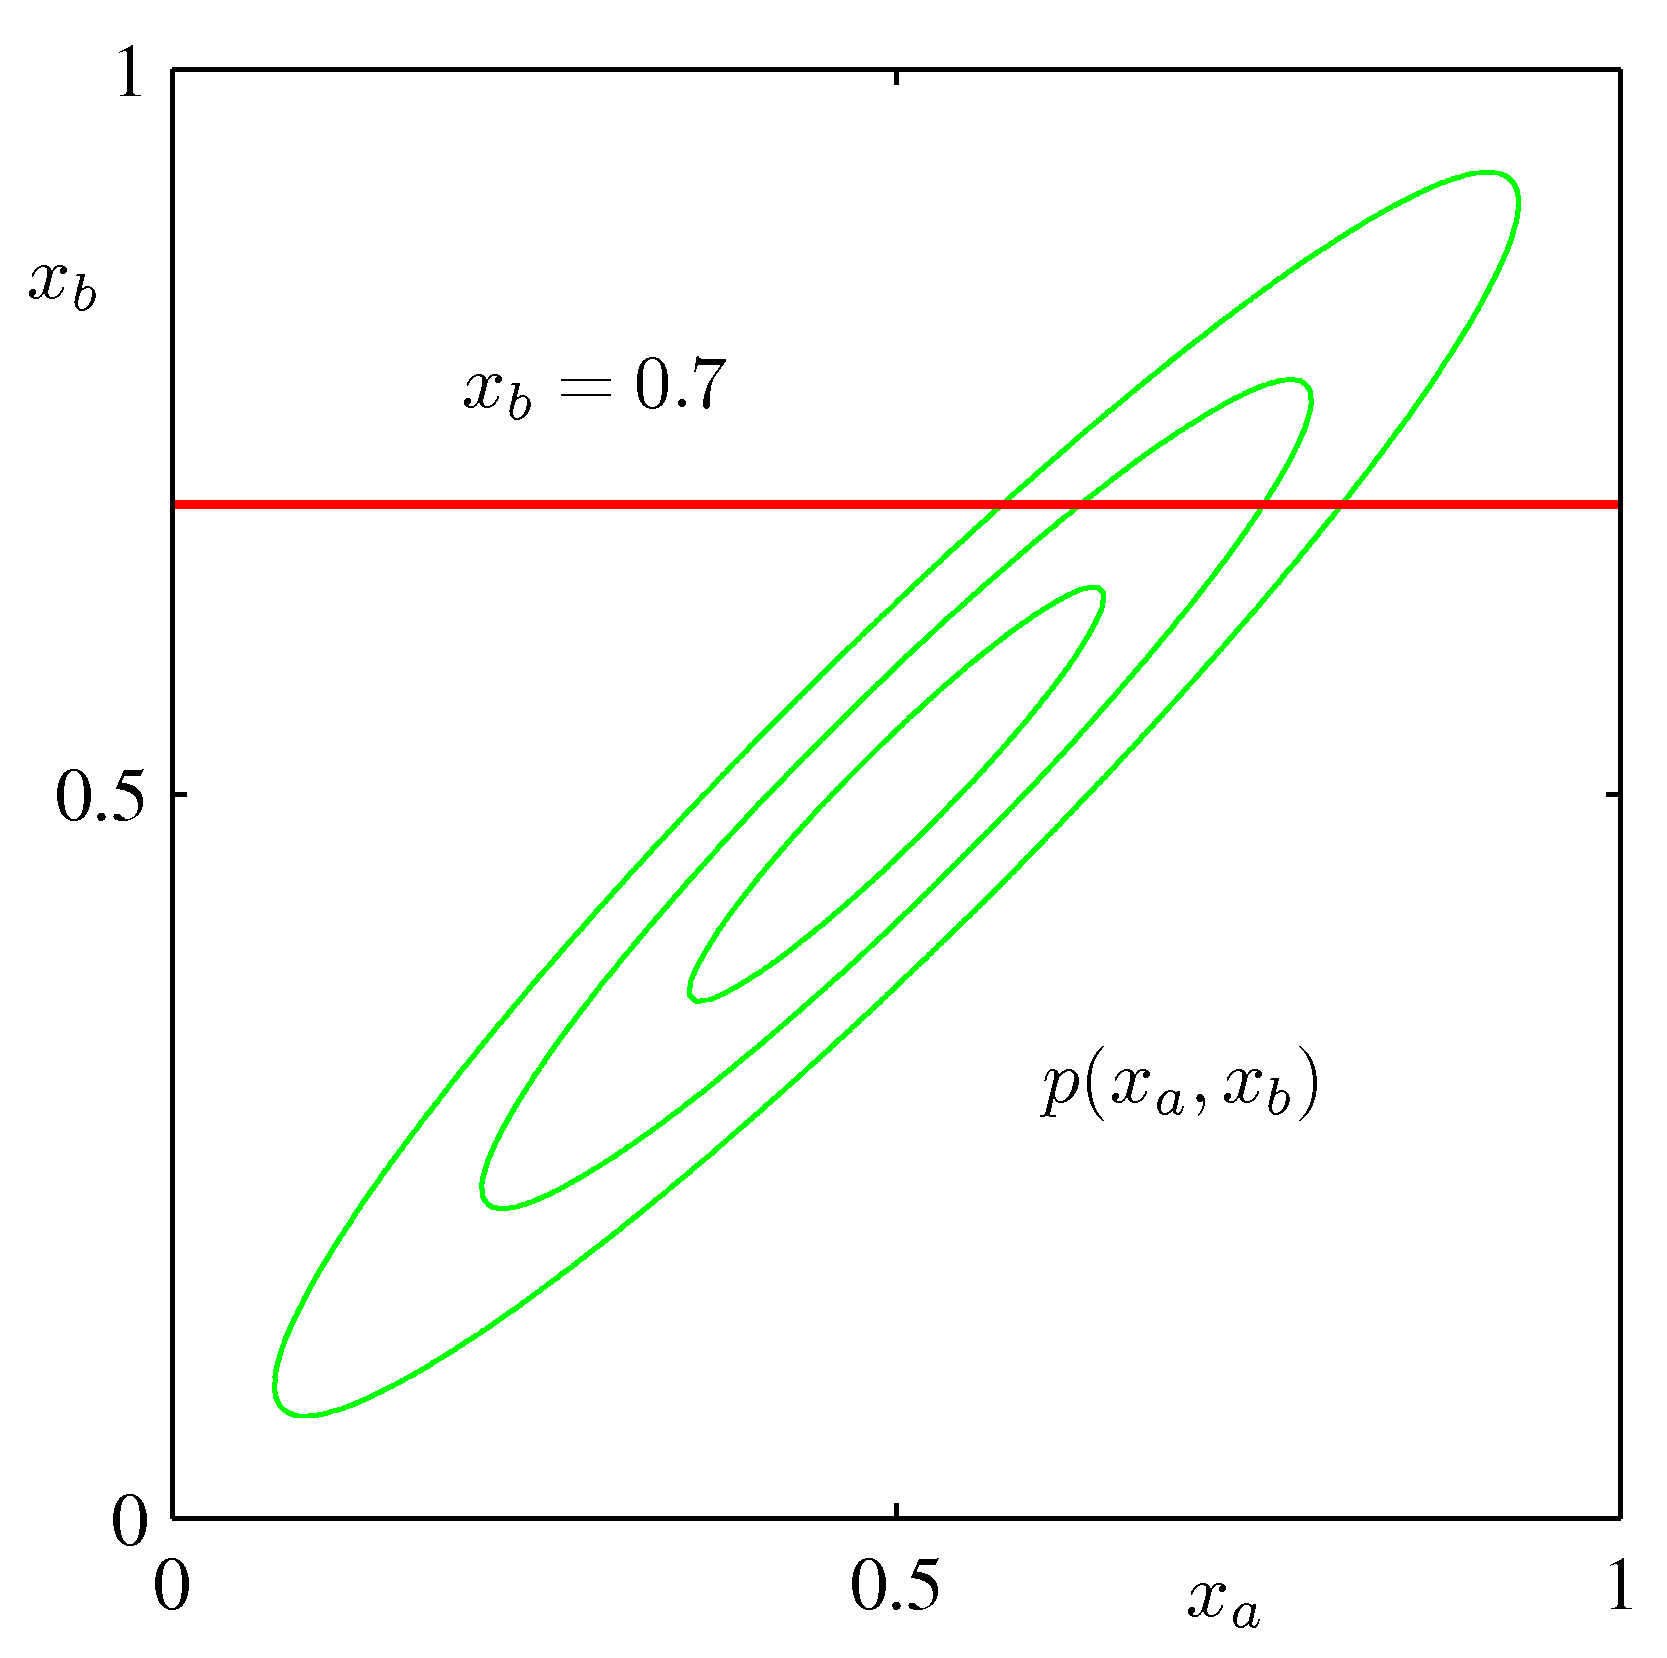
\includegraphics[scale=0.8]{Images/2-9a.png}
		\label{fig:2-9a}
		\end{minipage}
		\begin{minipage}[t]{0.5\linewidth}
		\centering
		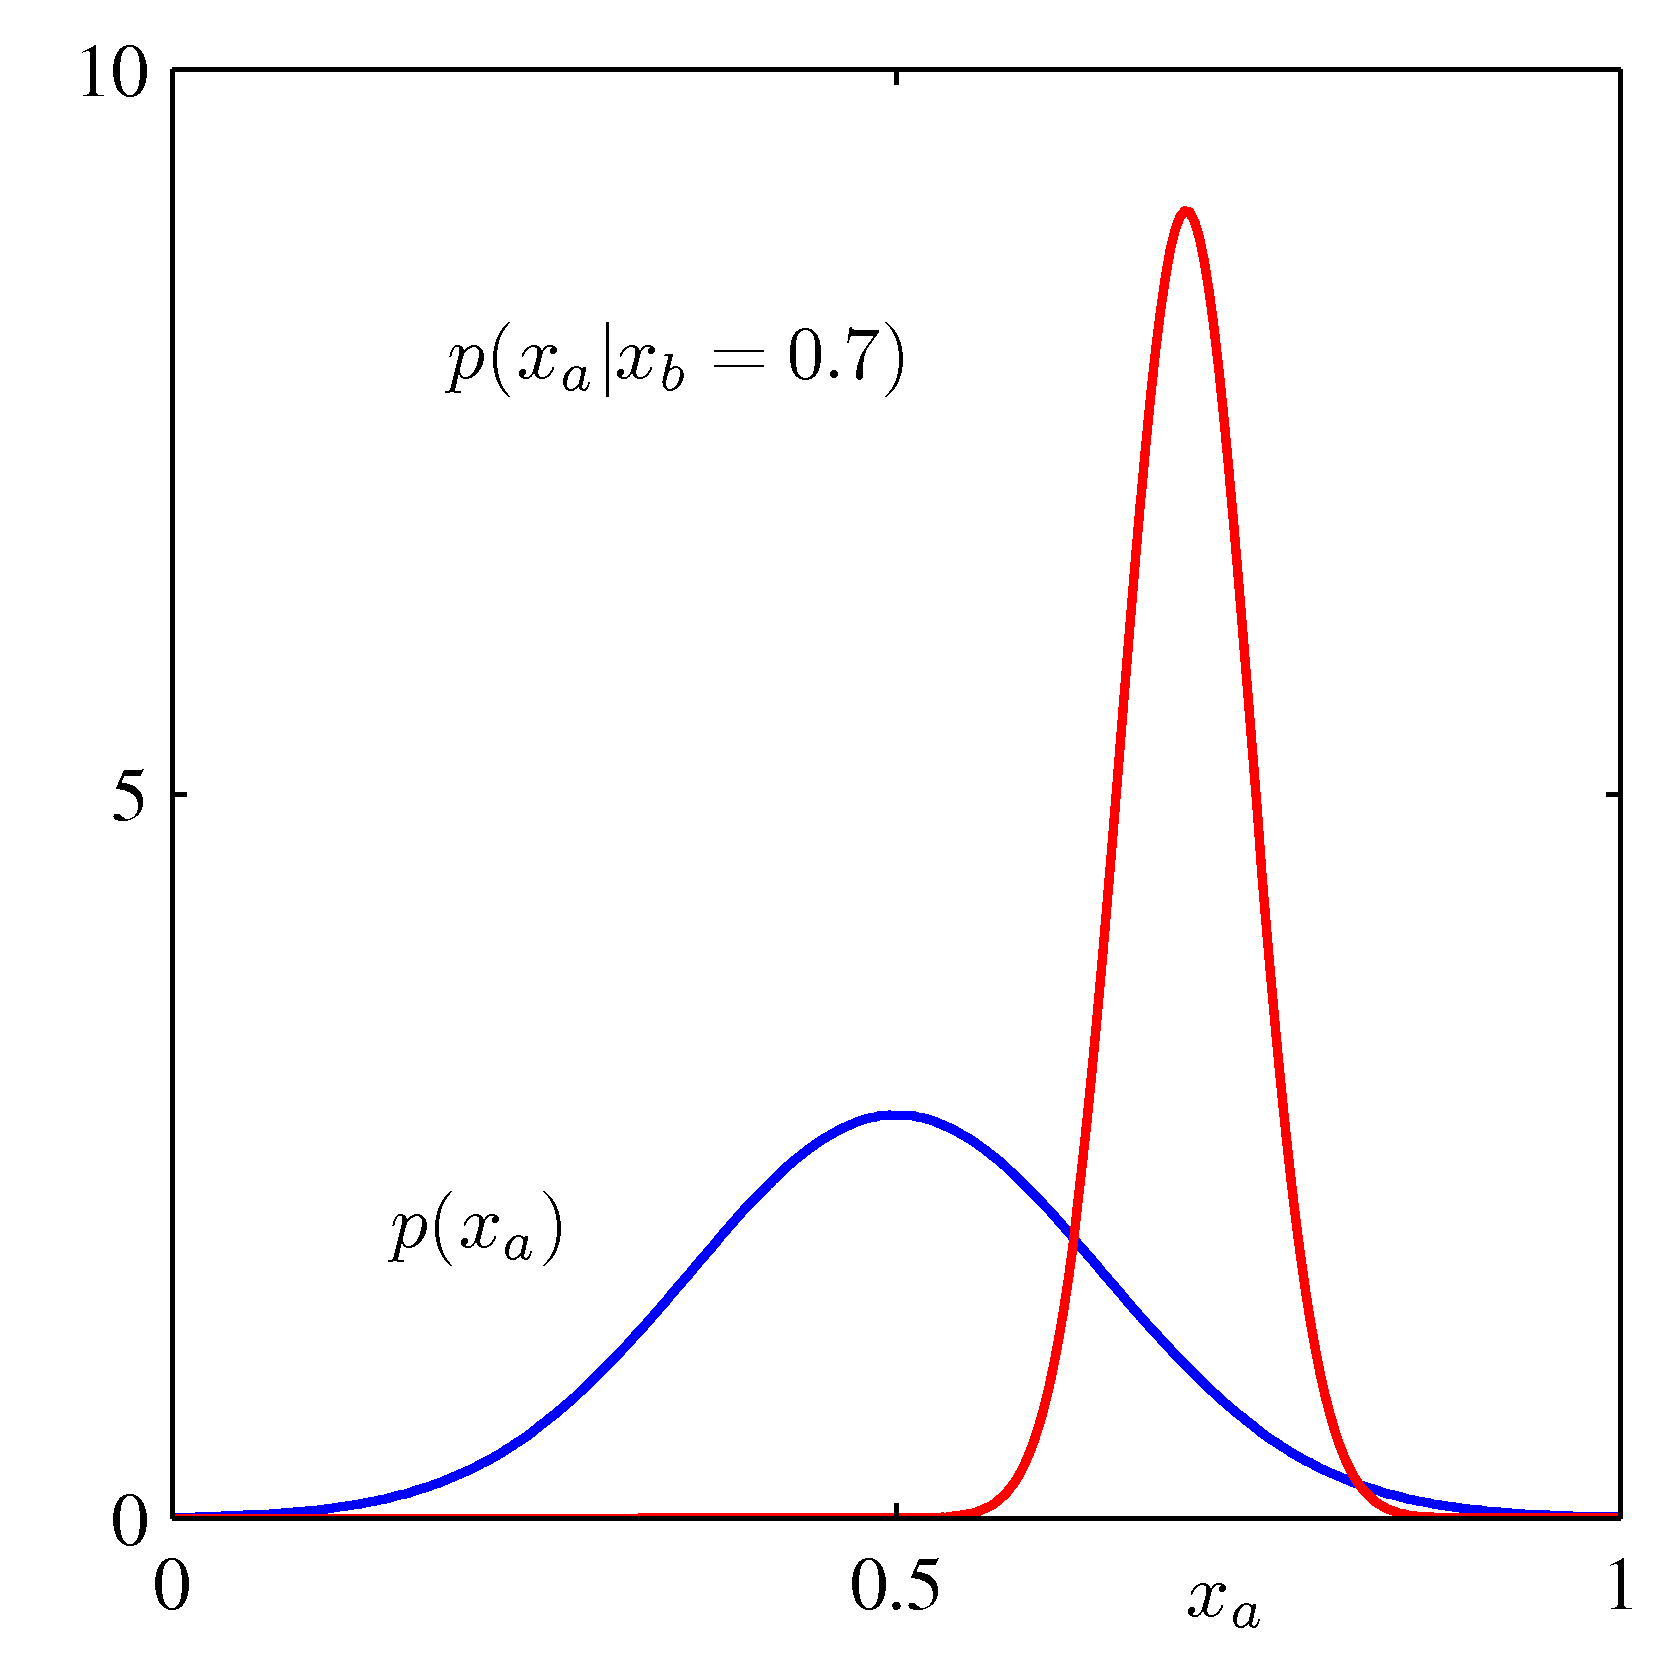
\includegraphics[scale=0.8]{Images/2-9b.png}
		\label{fig:2-9b}
		\end{minipage}
		\captionsetup{font={small}}
		\caption{左图展示的是一个二元高斯分布$p(x_a,x_b)$的轮廓线,右图展示的是边缘分布$p(x_a)$(蓝色曲线)和给定$x_b=0.7$情况下的条件分布$p(x_a|x_b)$(红色曲线)。}
	\end{figure}
	}
	\subsection{高斯变量的贝叶斯定理}
	\textnormal{
	在第2.3.1节和第2.3.2节中,我们研究了高斯分布$p(\bx)$,并将向量$\bx$拆分成两个子向量$\bx=(\bx_a,\bx_b)$,然后求取条件分布$p(\bx_a|\bx_b)$和边缘分布$p(\bx_a)$的表达式。我们发现条件分布$p(\bx_a|\bx_b)$是$\bx_b$的线性函数。现在我们假设有一个高斯边缘分布$p(\bx)$和一个高斯条件分布$p(\mathbf{y}|\bx)$,其中$p(\mathbf{y}|\bx)$的均值为$\bx$的线性函数,协方差则与$\bx$无关。这是线性高斯模型(linear Gaussian model, Roweis and Ghahramani, 1999)的一个典型案例,我们将在第8.1.4节中更加深入地学习。现在我们希望求取边缘分布$p(\mathbf{y})$和条件分布$p(\bx|\mathbf{y})$,这个问题将在后面的内容中经常出现,现在推导出一个一般的结果对以后会很有帮助。\\
	\indent 对于边缘分布和条件分布,可以这样表达:
	\begin{align}
		p(\bx)&=\mathcal{N}(\bx|\bfMu,\bfLambda^{-1}) \\
		p(\mathbf{y}|\bx)&=\mathcal{N}(\mathbf{y}|\mathbf{Ax+b},\mathbf{L}^{-1})
	\end{align}
	其中的$\bfMu$,$\mathbf{A}$和$\mathbf{b}$为控制均值的参数,$\bfLambda$和$\mathbf{L}$均为精度矩阵。如果$\bx$的维数为$M$,$\mathbf{y}$的维数为$D$,那么矩阵$\mathbf{A}$就是$D \times M$维的。\\
	\indent 首先求取$\bx$和$\mathbf{y}$的联合分布。定义
	\begin{equation}
		\mathbf{z}=\left(\begin{matrix}
			\bx \\ \mathbf{y}
		\end{matrix}\right)
	\end{equation}
	然后求联合分布的对数
	\begin{equation}
	\begin{split}
		\ln p(\mathbf{z}) &= \ln p(\bx) + \ln p(\mathbf{y}|\bx) \\
		&=-\frac{1}{2}(\bx-\bfMu)^{\rmT}\bfLambda(\bx-\bfMu) -\frac{1}{2}(\mathbf{y}-\mathbf{Ax}-\mathbf{b})^{\rmT}\mathbf{L}(\mathbf{y}-\mathbf{Ax}-\mathbf{b})+\mathrm{const}
	\end{split}
	\end{equation}
	其中“const”表示与$\bx$和$\mathbf{y}$无关的部分。和以前一样,可以看出这是一个关于$\mathbf{z}$的二次型函数,所以$p(\mathbf{z})$是一个高斯分布。为了找到这个高斯分布的精度矩阵,可以对(2.102)中的二阶项进行一些处理:
	\begin{equation}
	\begin{split}
		&-\frac{1}{2}\bx^{\rmT}(\bfLambda + \mathbf{A}^{\rmT}\mathbf{LA})\bx-\frac{1}{2}\mathbf{y}^{\rmT}\mathbf{Ly}+\frac{1}{2}\mathbf{y}^{\rmT}\mathbf{LAx}+\frac{1}{2}\bx^{\rmT}\mathbf{A}^{\rmT}\mathbf{Ly}\\
		= &-\frac{1}{2}\left(\begin{matrix} \bx \\ \mathbf{y}\end{matrix}\right)^{\rmT}\left(\begin{matrix}\bfLambda+\mathbf{A}^{\rmT}\mathbf{LA} & -\mathbf{A}^{\rmT}\mathbf{L} \\ -\mathbf{LA} & \mathbf{L}\end{matrix}\right) \left(\begin{matrix}\bx \\ \mathbf{y}\end{matrix}\right) = -\frac{1}{2}\mathbf{z^{\rmT}Rz}
	\end{split}
	\end{equation}
	所以$\mathbf{z}$的高斯分布的精度矩阵为
	\begin{equation}
		\mathbf{R}=\left(\begin{matrix}\bfLambda + \mathbf{A}^{\rmT}\mathbf{LA} & -\mathbf{A}^{\rmT}\mathbf{L} \\ -\mathbf{LA} & \mathbf{L}\end{matrix}\right)
	\end{equation}
	协方差矩阵可以通过将精度矩阵求逆来获得,根据(2.76),\textcolor{red}{\textbf{——习题 2.29}}
	\begin{equation}
		\mathrm{cov}[\mathbf{z}]=\mathbf{R}^{-1}=\left(\begin{matrix}
		 \bfLambda^{-1} & \bfLambda^{-1}\mathbf{A}^{\rmT} \\ 
		 \mathbf{A}\bfLambda^{-1} & \mathbf{L}^{-1}+\mathbf{A}\bfLambda^{-1} \mathbf{A}^{\rmT}
		 \end{matrix}\right)
	\end{equation}
	\indent 类似地,$\mathbf{z}$的高斯分布的均值可以通过(2.102)中的线性项确定:
	\begin{equation}
		\bx^{\rmT}\bfLambda\bfMu-\bx^{\rmT}\mathbf{A}^{\rmT}\mathbf{Lb}+\mathbf{y}^{\rmT}\mathbf{Lb}=\left(\begin{matrix}
			\bx \\ \mathbf{y}
		\end{matrix}\right)^{\rmT} 
		\left(\begin{matrix}
			\bfLambda\bfMu-\mathbf{A}^{\rmT}\mathbf{Lb} \\
			\mathbf{Lb}
		\end{matrix}\right)
	\end{equation}
	根据多元高斯分布的二次型完成平方项的结果(2.71),可以看出$\mathbf{z}$的均值为
	\begin{equation}
		\mathbb{E}[\mathbf{z}]=\mathbf{R}^{-1}\left(\begin{matrix}
			\bfLambda\bfMu-\mathbf{A}^{\rmT}\mathbf{Lb} \\ \mathbf{Lb}
		\end{matrix}\right)
	\end{equation}
	利用(2.105),可以得到\textcolor{red}{\textbf{——习题 2.30}}
	\begin{equation}
		\mathbb{E}[\mathbf{z}]=\left(\begin{matrix}
			\bfMu \\ \mathbf{A}\bfMu+\mathbf{b}
		\end{matrix}\right)
	\end{equation}
	\indent 接下来我们求取边缘分布$p(\mathbf{y})$的表达式,也就是对$\mathbf{x}$求边缘化。回想一下前面对于高斯随机向量的一个分量求边缘分布时,利用分块协方差矩阵可以很容易地进行表达。\textcolor{red}{\textbf{——第2.3节\ }}特别地,其均值和方差分别为(2.92)和(2.93)中所示的那样。利用(2.105)和(2.108),可以看出边缘分布$p(\mathbf{y})$的均值和协方差分别为
	\begin{align}
		\mathbb{E}[\mathbf{y}]&=\mathbf{A} \bfMu + \mathbf{b} \\
		\mathrm{cov}[\mathbf{y}]&=\mathbf{L}^{-1}+\mathbf{A}\bfLambda^{-1}\mathbf{A}^{\rmT}
	\end{align}
	有一种特殊情况——如果$\mathbf{A}=\mathbf{I}$,那么以上内容就会退化为两个高斯分布的卷积,且卷积的均值就是两个高斯分布均值的和,卷积的协方差就是两个高斯分布协方差的和。\\
	\indent 最后,我们要求取条件分布$p(\bx|\mathbf{y})$的表达式。再回想一下前面的内容,根据(2.73)和(2.75),条件分布的表达式用分块精度矩阵表示是最简单的。将它们代入(2.105)和(2.108),可以得到条件分布$p(\bx|\mathbf{y})$的均值和协方差为
	\begin{align}
		\mathbb{E}[\bx|\mathbf{y}]&=(\bfLambda+\mathbf{A}^{\rmT}\mathbf{LA})^{-1}\{\mathbf{A}^{\rmT}\mathbf{L(y-b)}+\bfLambda\bfMu\} \\
		\mathrm{cov}[\bx|\mathbf{y}]&=(\bfLambda+\mathbf{A}^{\rmT}\mathbf{LA})^{-1}
	\end{align}
	\indent 条件分布的求取事实上可以看成是贝叶斯定理的应用实例。我们可以认为分布$p(\bx)$是关于$\bx$的先验分布。一旦得到了$\mathbf{y}$的值,那么条件分布$p(\bx|\mathbf{y})$就表示对应的关于$\bx$的后验分布。在求出了边缘分布和条件分布之后,我们可以用$p(\bx|\mathbf{y})p(\mathbf{y})$的形式写出联合分布$p(\mathbf{z})=p(\bx)p(\mathbf{y}|\bx)$。\\
	\insertline \\
	\color{red} $\bullet$ \textbf{\ 高斯分布的边缘分布和条件分布} \color{black} \\
	\indent 给定一个关于$\bx$的边缘高斯分布和给定$\bx$的条件下$\mathbf{y}$的条件高斯分布:
	\begin{align}
		p(\bx) &= \mathcal{N}(\bx|\bfMu,\bfLambda^{-1})\\
		p(\mathbf{y}|\bx)&=\mathcal{N}(\mathbf{y}|\mathbf{Ax+b},\mathbf{L}^{-1})
	\end{align}
	那么关于$\mathbf{y}$的边缘分布和给定$\mathbf{y}$的条件下$\bx$的条件分布分别为
	\begin{align}
		p(\mathbf{y})&=\mathcal{N}(\mathbf{y}|\mathbf{A}\bfMu+\mathbf{b},\mathbf{L}^{-1}+\mathbf{A}\bfLambda^{-1}\mathbf{A}^{\rmT}) \\
		p(\bx|\mathbf{y})&=\mathcal{N}(\bx|\bfSigma\{\mathbf{A}^{\rmT}\mathbf{L(y-b)}+\bfLambda\bfMu\},\bfSigma)
	\end{align}
	其中
	\begin{equation}
		\bfSigma=(\bfLambda+\mathbf{A}^{\rmT}\mathbf{LA})^{-1}
	\end{equation}
	\insertline
	}
	\subsection{高斯分布的最大似然}
	\textnormal{
	给定一个数据集$\mathbf{X}=(\bx_1,...,\bx_N)^{\rmT}$,其中的数据$\{\bx_n\}$是从一个多元高斯分布中相互独立地抽取出来的,我们可以通过最大似然的方法求出分布的参数。对数似然函数为
	\begin{equation}
		\ln p(\mathbf{X}|\bfMu,\bfSigma)=-\frac{ND}{2}\ln (2\pi) -\frac{N}{2}\ln |\bfSigma| -\frac{1}{2}\sum_{n=1}^N(\bx_n-\bfMu)^{\rmT}\bfSigma^{-1}(\bx_n-\bfMu)
	\end{equation}
	通过一个简单的处理,可以看出似然函数对数据集的依赖仅限于如下两项:
	\begin{equation}
		\sum_{n=1}^N\bx_n , \sum_{n=1}^N\bx_n\bx_n^{\rmT}
	\end{equation}
	这两项内容就是高斯分布的充分统计量。利用(C.19),将对数似然函数关于$\bfMu$求导:\textcolor{red}{\textbf{——附录 C}}
	\begin{equation}
		\frac{\partial}{\partial \bfMu}\ln p(\mathbf{X}|\bfMu,\bfSigma)=\sum_{n=1}^N\bfSigma^{-1}(\bx_n-\bfMu)
	\end{equation}
	并令该导数为0,可以得到均值的最大似然解
	\begin{equation}
		\bfMu_{\mathrm{ML}}=\frac{1}{N}\sum_{n=1}^N\bx_n
	\end{equation}
	其实就是整个数据集的均值。(2.118)关于$\bfSigma$的最大值要涉及的内容就更多了。最简单的办法,就是忽略对称约束,并证明最后的结果还是满足所要求的对称性的。\textcolor{red}{\textbf{——习题 2.34}\ }这个内容的推导可以参考Magnus and Neudecker(1999)的相关工作,其中明确加上了对称性和正定性的约束。结果为
	\begin{equation}
		\bfSigma_{\mathrm{ML}} = \frac{1}{N}\sum_{n=1}^N(\bx_n-\bfMu_{\mathrm{ML}})(\bx_n-\bfMu_{\mathrm{ML}})^{\rmT}
	\end{equation}
	其中包含了$\bfMu_{\mathrm{ML}}$,因为这个结果是关于$\bfMu$和$\bfSigma$的最大值。需要注意的是,关于$\bfMu_{\mathrm{ML}}$的解(2.121)并不依赖于$\bfSigma_{\mathrm{ML}}$,所以我们可以先求$\bfMu_{\mathrm{ML}}$,然后再求$\bfSigma_{\mathrm{ML}}$。\\
	\indent 如果我们要求取真实分布下的最大似然解,最后的结果就是\textcolor{red}{\textbf{——习题 2.35}}
	\begin{align}
		\mathbb{E}[\bfMu_{\mathrm{ML}}] &= \bfMu\\
		\mathbb{E}[\bfSigma_{\mathrm{ML}}] &=\frac{N-1}{N}\bfSigma
	\end{align}
	可以看出,基于最大似然估计的均值期望等于真实的均值。然而,协方差矩阵的最大似然估计却小于真实的协方差矩阵,无疑是一个有偏估计。我们可以通过定义另一个估计$\widetilde{\bfSigma}$来修正这个偏差:
	\begin{equation}
		\widetilde{\bfSigma}=\frac{1}{N-1}\sum_{n=1}^N(\bx_n-\bfMu_{\mathrm{ML}})(\bx_n-\bfMu_{\mathrm{ML}})^{\rmT}
	\end{equation}
	很明显,(2.122)和(2.124)中,$\widetilde{\bfSigma}$的期望等于$\bfSigma$。
	}
	\subsection{顺序估计}
	\textnormal{
	关于高斯分布中参数的最大似然解的讨论使得我们可以对最大似然的顺序估计这个问题进行更加广泛的讨论。顺序方法使得数据可以逐一处理然后马上丢弃,这对实时应用非常重要,同时也对无法一次性完全处理的大数据集有很大的帮助。\\
	\indent 对于(2.121)中均值的最大似然解$\bfMu_{\mathrm{ML}}$,在$N$组数据中可以分别表示为$\bfMu_{\mathrm{ML}}^{(N)}$。如果我们把与最后一个数据$\bx_N$相关的内容剖析出来,可以得到
	\begin{equation}
	\begin{split}
		\bfMu_{\mathrm{ML}}^{(N)} &= \frac{1}{N}\sum_{n=1}^N \bx_n \\
		&= \frac{1}{N}\bx_N+\frac{1}{N}\sum_{n=1}^{N-1}\bx_n \\
		&= \frac{1}{N}\bx_N + \frac{N-1}{N}\bfMu_{\mathrm{ML}}^{(N-1)} \\
		&= \bfMu_{\mathrm{ML}}^{(N-1)}+\frac{1}{N}(\bx_{N}-\bfMu_{\mathrm{ML}}^{(N-1)})
	\end{split}
	\end{equation}
	这个结果有一个相当精巧的解释,如下所述。在经过$N-1$个数据的洗礼后,我们利用$\bfMu_{\mathrm{ML}}^{(N-1)}$估计了$\bfMu$。现在又有了一个新的数据$\bx_N$,我们要利用这个新的数据来修正之前的估计,得到一个新的估计$\bfMu_{\mathrm{ML}}^{(N)}$,而修正的尺度为$1/N$,修正的方向为“误差信号”$(\bx_N-\bfMu_{\mathrm{ML}}^{(N-1)})$。需要注意的是,随着$N$的增加,连续数据点的贡献会变小。\\
	\indent (2.126)会给出与批处理结果(2.121)一样的结果,因为这两个公式是完全等价的。然而,这条顺序算法的路线并不一定总能走得通,所以我们需要找到更加一般的顺序学习算法,那就是Robbins-Monro算法。对于一对随机变量$\theta$和$z$,其联合分布为$p(\theta,z)$,那么在给定$\theta$的条件下$z$的条件期望可以定义一个函数$f(\theta)$:
	\begin{equation}
		f(\theta)=\mathbb{E}[z|\theta]=\int zp(z|\theta)\ \mathrm{d}z
	\end{equation}
	如图2.10所示。这样的函数称为回归函数(regression function)。\\
	\indent 我们的目标是求出方程$f(\theta^{\star})=0$的根$\theta^{\star}$。如果我们有一个很大的关于$z$和$\theta$的数据集,那就可以对回归函数进行直接的建模,并估计它的根。不过,现在假设我们一次仅拿到一个$z$的值,并希望用顺序估计的方法来得到$\theta^{\star}$。如下这个解决问题的一般程序由Robbins and Monro (1951)的研究中给出。我们假设$z$的条件方差是有限的,那么
	\begin{equation}
		\mathbb{E}[(z-f)^2|\theta]<\infty
	\end{equation}
	一般地,我们同样会考虑$\theta>\theta^{\star}$时$f(\theta)>0$,以及$\theta<\theta^{\star}$时$f(\theta)<0$的情况,如图2.10所示。
	\begin{figure}[ht]
		\centering
		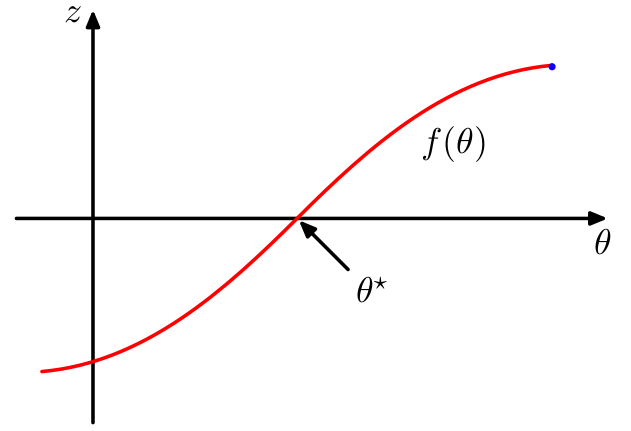
\includegraphics[scale=0.3]{Images/2-10.png}
		\captionsetup{font={small}}
		\caption{两个相关的随机变量$z$和$\theta$及根据条件期望$\mathbb{E}[z|\theta]$给出的回归函数$f(\theta)$的示意图。Robbins-Monro算法给出了求取根$\theta^{\star}$的一般顺序步骤。}
		\label{fig:2-10}
	\end{figure}
	\\
	\indent Robbins-Monro算法接下来定义了对于根$\theta^{\star}$的估计序列:
	\begin{equation}
		\theta^{(N)}=\theta^{(N-1)}-a_{N-1}z(\theta^{(N-1)})
	\end{equation}
	其中的$z(\theta^{(N)})$为当$\theta$的取值为$\theta^{(N)}$时$z$的数值。常数$\{a_N\}$表示的是一个满足以下条件的正数序列:
	\begin{align}
		\lim_{N \rightarrow \infty}a_N &=0 \\
		\sum_{N=1}^{\infty}a_n &=\infty \\
		\sum_{N=1}^{\infty}a_N^2 &< \infty
	\end{align}
	可以证明根据(2.129)得到的估计序列确实会收敛到根$\theta^{\star}$而且概率为1。需要注意的是,第一个条件(2.130)确保了连续修正的幅度逐渐减小,使得该过程可以收敛到某一极限值;第二个条件(2.131)是为了确保算法不会在缺少根的时候收敛;第三个条件(2.132)是为了确保累计噪声的方差是有限的,所以不会破坏收敛性。\\
	\indent 现在我们研究一下如何利用Robbins-Monro算法顺序求解一个一般的最大似然问题。根据定义,最大似然问题的解$\theta_{\mathrm{ML}}$是负对数似然函数的驻点,于是一定满足
	\begin{equation}
		\left.\frac{\partial}{\partial\theta}\left\{-\frac{1}{N}\sum_{n=1}^N \ln p(x_n|\theta)\right\}\right|_{\theta_{\mathrm{ML}}}=0
	\end{equation}
	将求导与求和交换位置,并取极限$N \rightarrow \infty$,可以得到
	\begin{equation}
		-\lim_{N\rightarrow\infty}\frac{1}{N}\sum_{n=1}^N\frac{\partial}{\partial\theta}\ln p(x_n|\theta)=\mathbb{E}_x\left[-\frac{\partial}{\partial\theta}\ln p(x|\theta)\right]
	\end{equation}
	于是可以看出求取最大似然解对应着求取回归方程的根。于是就可以利用Robbins-Monro算法,形式为
	\begin{equation}
		\theta^{(N)}=\theta^{(N-1)}-a_{N-1}\frac{\partial}{\partial\theta^{(N-1)}}[-\ln p(x_N|\theta^{(N-1)})]
	\end{equation}
	\indent 作为一个特例,我们再次把目光转向高斯分布均值的顺序估计,其中的参数$\theta^{(N)}$就是高斯分布均值的估计$\mu_{\mathrm{ML}}^{(N)}$,随机变量$z$为
	\begin{equation}
		z=-\frac{\partial}{\partial\mu_{\mathrm{ML}}}\ln p(x|\mu_{\mathrm{ML}},\sigma^2)=-\frac{1}{\sigma^2}(x-\mu_{\mathrm{ML}})
	\end{equation}
	于是$z$的分布为高斯分布,其均值为$-(\mu-\mu_{\mathrm{ML}})$,如图2.11所示。将(2.136)代入(2.135),可以得到(2.126)的一元变量形式,$a_N$的取值为$a_N=\sigma^2/N$。需要注意的是,尽管我们以一元变量为例进行了推导,但整个过程,包括(2.130)-(2.132)对$a_N$的限制条件,对于多元变量都是完全等价的(Blum, 1965)。
	\begin{figure}[ht]
		\centering
		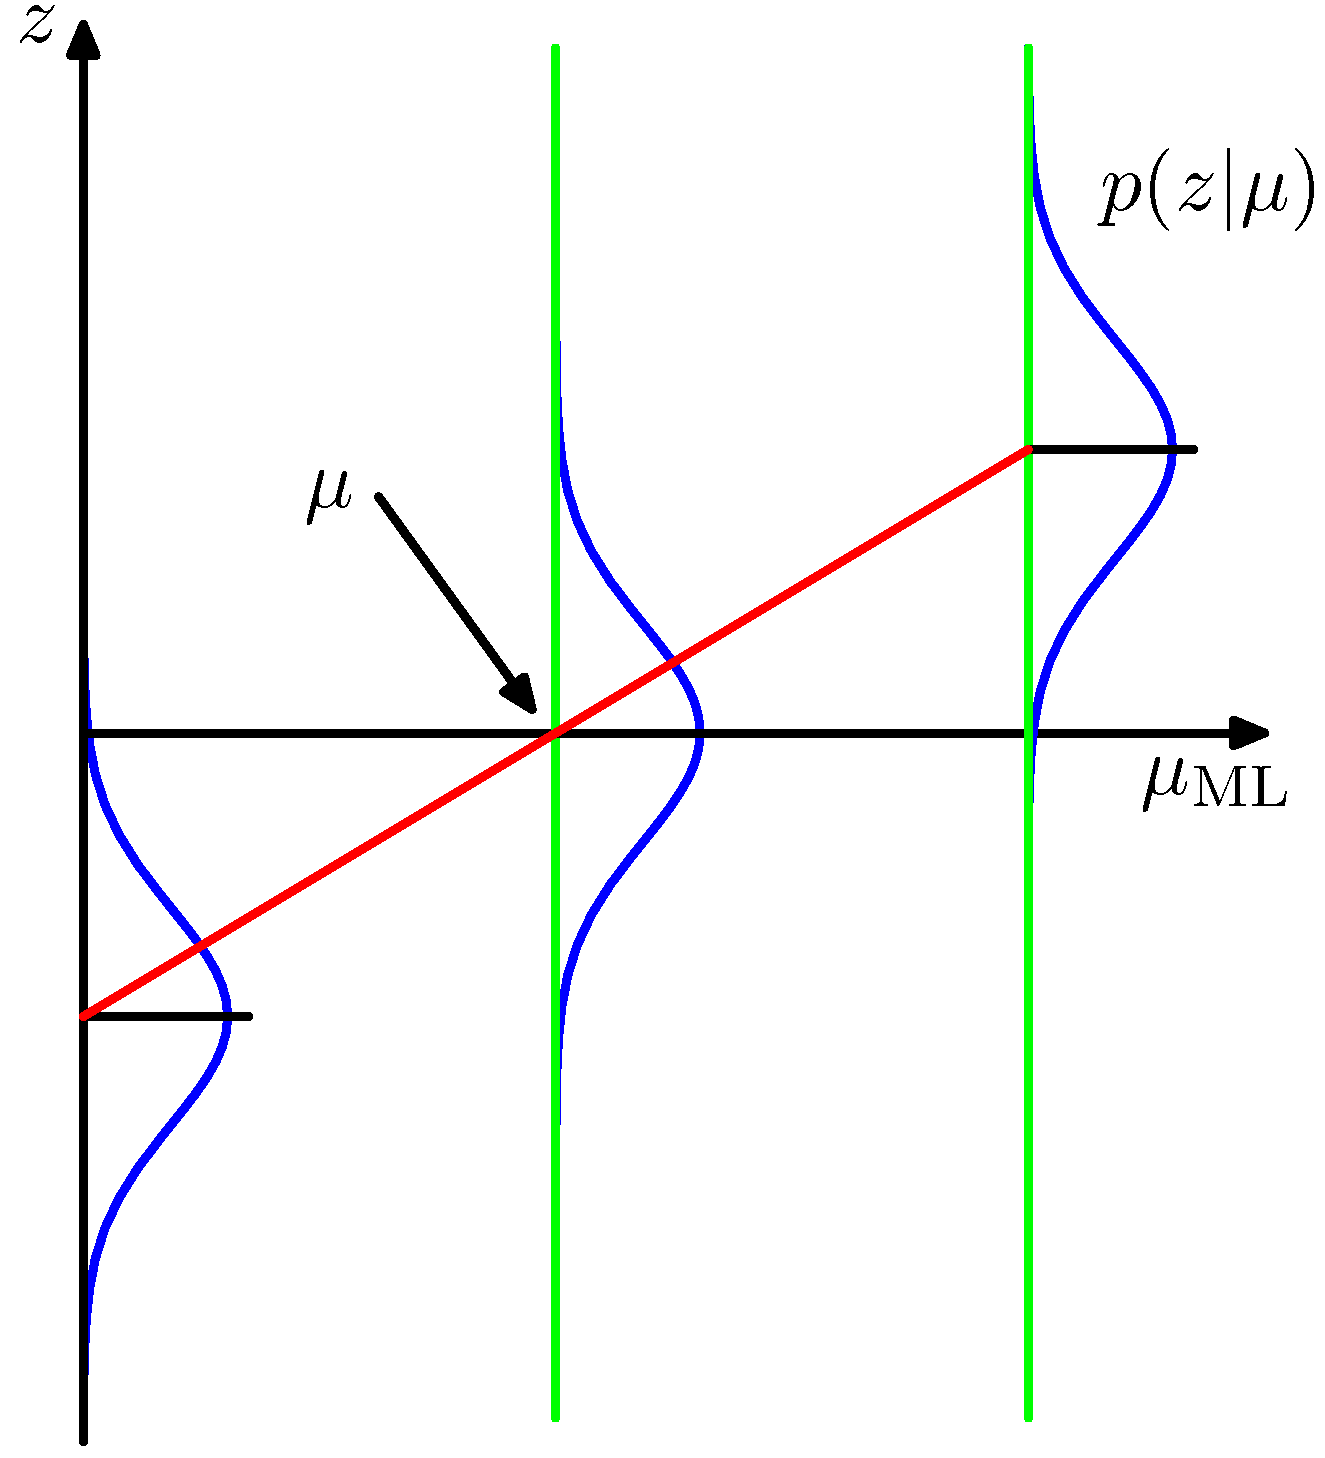
\includegraphics[scale=0.8]{Images/2-11.png}
		\captionsetup{font={small}}
		\caption{在高斯分布中,如图2.10所示的回归函数的形式为一条直线,如图中红色直线所示。在这种情况下,随机变量$z$对应着负对数似然函数的导数,取值为$-(x-\mu_{\mathrm{ML}})/\sigma^2$,定义了回归函数的期望是一条直线,取值为$-(\mu-\mu_{\mathrm{ML}})/\sigma^2$。回归方程的根对应着真实的均值$\mu$。}
		\label{fig:2-11}
	\end{figure}
	}
	\subsection{高斯分布中的贝叶斯推断}
	\textnormal{
	最大似然这个框架为参数$\bfMu$和$\bfSigma$给出了点估计。现在我们通过引入各个参数的先验分布来进行贝叶斯估计。我们先从最简单的一元高斯随机变量$x$开始。假设方差$\sigma^2$已知,我们要利用$N$组数据$\bx=\{x_1,...,x_N\}$来推断均值$\mu$。似然函数是给定$\mu$的条件下得到这些数据的概率,现在将似然函数视为关于$\mu$的函数,也就是
	\begin{equation}
		p(\sfx|\mu)=\prod_{n=1}^Np(x_n|\mu)=\frac{1}{(2\pi\sigma^2)^{N/2}}\exp\left\{-\frac{1}{2\sigma^2}\sum_{n=1}^N(x_n-\mu)^2\right\}
	\end{equation}
	需要再次强调一下,似然函数$p(\sfx|\mu)$并不是一个关于$\mu$的概率分布,而且并不满足归一化条件。\\
	\indent 不过可以看出,似然函数中指数项的指数为$\mu$的二次型。所以如果我们将$p(\mu)$的先验分布设置为高斯分布,那自然是似然函数的一个共轭分布,因为对应的后验分布将会是两个指数为$\mu$的二次型的指数项相乘,所以也是一个高斯分布。所以设先验分布为
	\begin{equation}
		p(\mu)=\mathcal{N}(\mu|\mu_0,\sigma_0^2)
	\end{equation}
	且后验分布为
	\begin{equation}
		p(\mu|\sfx) \propto p(\sfx|\mu)p(\mu)
	\end{equation}
	对于指数进行一个简单的完成平方项的操作之后,后验分布可以写成
	\begin{equation}
		p(\mu|\sfx)=\mathcal{N}(\mu|\mu_N,\sigma_N^2)
	\end{equation}
	其中的
	\begin{align}
		\mu_N &=\frac{\sigma^2}{N\sigma_0^2+\sigma^2}\mu_0+\frac{N\sigma_0^2}{N\sigma_0^2+\sigma^2}\mu_{\mathrm{ML}}\\
		\frac{1}{\sigma_N^2}&=\frac{1}{\sigma_0^2}+\frac{N}{\sigma^2}
	\end{align}
	其中的$\mu_{\mathrm{ML}}$为$\mu$的最大似然解,由样本均值给出:
	\begin{equation}
		\mu_{\mathrm{ML}}=\frac{1}{N}\sum_{n=1}^Nx_n
	\end{equation}
	\indent 在这里花一点时间研究一下后验分布的均值和方差的形式是比较值得的。首先一件需要注意的事情是,(2.141)给出的均值$\mu$的均值事实上是先验均值$\mu_0$和最大似然解$\mu_{\mathrm{ML}}$之间的妥协或者说权衡。如果数据的数量$N=0$,那么(2.141)就退化成了先验均值;而如果$N \rightarrow 0$,那么后验均值就变成了最大似然解。类似地,对于(2.142)中后验分布的方差,可以看出用方差的倒数——也就是精度来表示更加自然。另外,精度是可加的,所以可以将先验分布的精度加上每个数据带来的精度修正,从而得到后验分布的精度。随着数据数量的增加,精度也会随之提升,也就意味着后验分布的方差也会随之下降。在完全没有数据的情况下,那么后验方差就是先验方差;如果数据数量$N \rightarrow 0$,那么方差$\sigma_N^2$将趋近于0,后验分布将会在最大似然解处趋近于无限大。所以可以看出,(2.143)对于$\mu$的最大似然解给出的点估计会在数据数量趋近于无限时在贝叶斯推断中再次浮现出来。对于有限的$N$,如果我们取极限$\sigma_0^2 \rightarrow \infty$,那么先验的方差就是无限大的,那么(2.141)中的后验均值就退化为最大似然解了,根据(2.142),后验方差为$\sigma_N^2=\sigma^2/N$。\\
	\indent 如图2.12所示为高斯分布均值的贝叶斯推断的分析。这个结论可以直接推广到已知协方差但未知均值的$D$维高斯随机变量$\bx$的情况中。\textcolor{red}{\textbf{——习题 2.40}}
	\begin{figure}[ht]
		\centering
		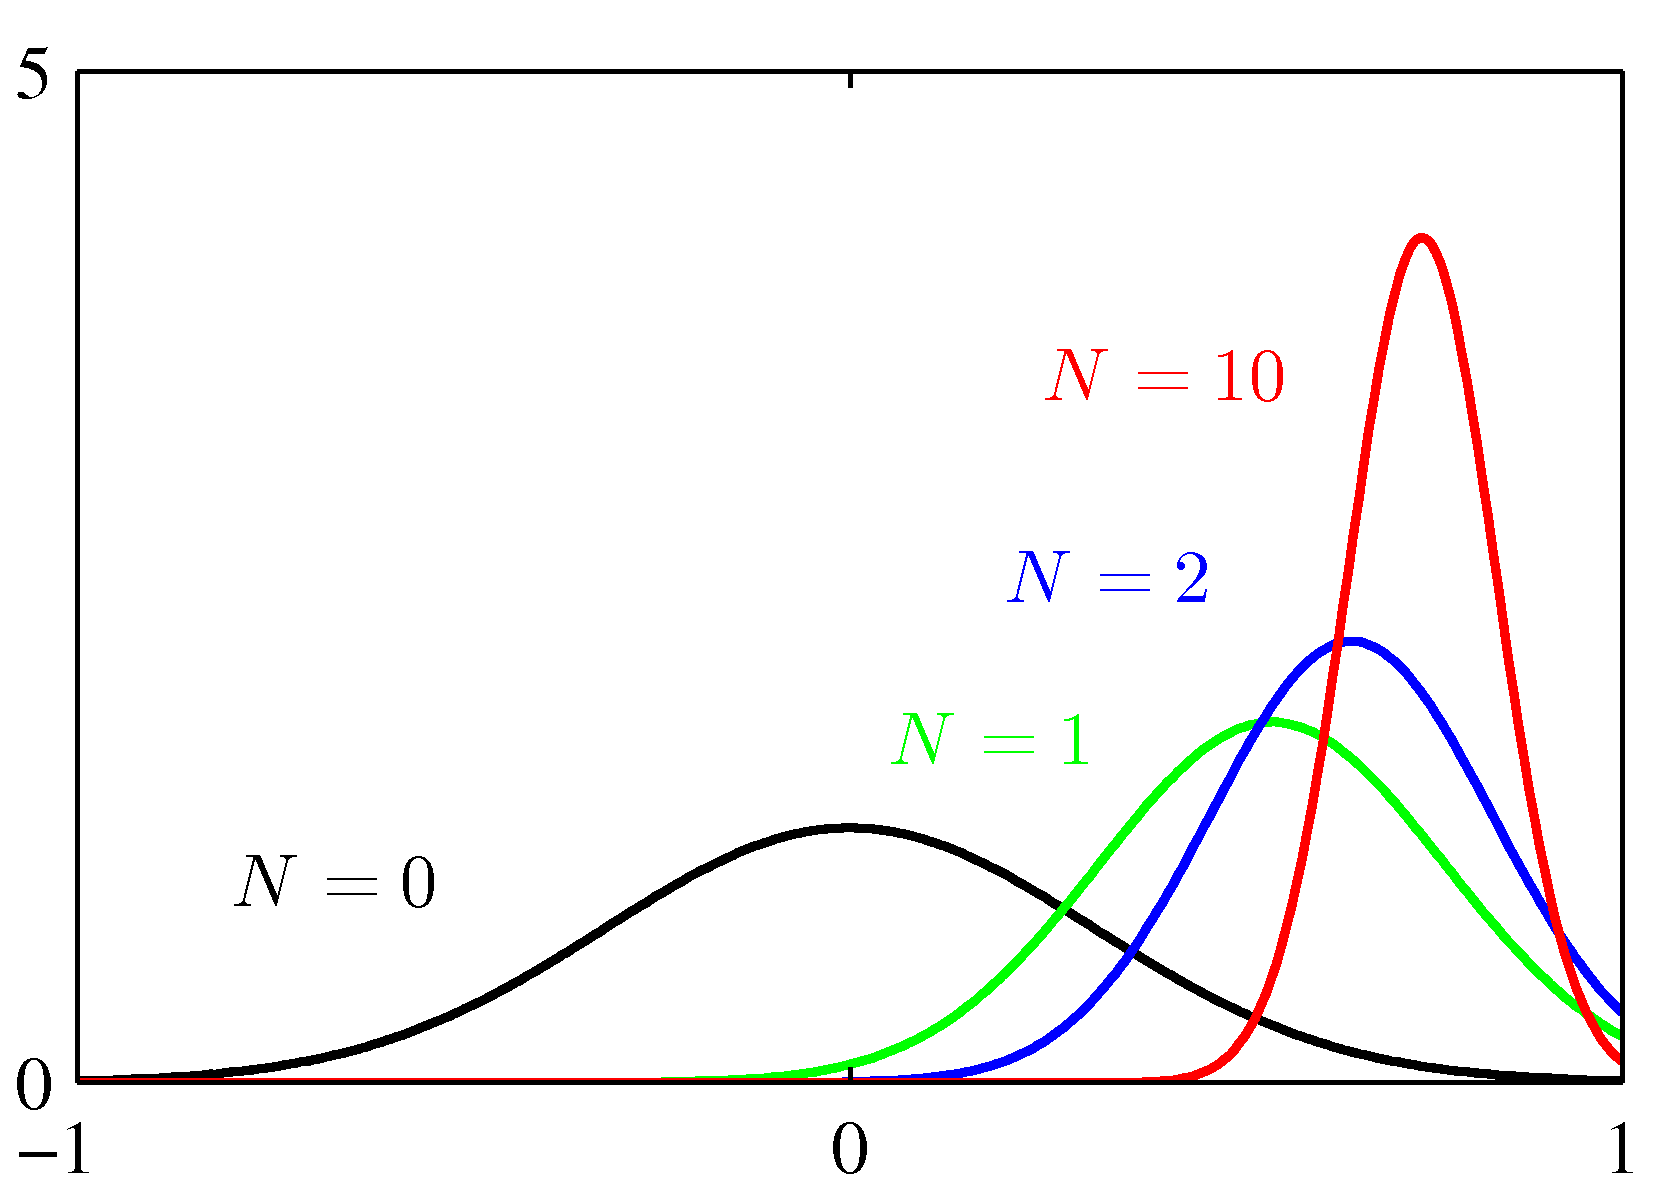
\includegraphics[scale=0.8]{Images/2-12.png}
		\captionsetup{font={small}}
		\caption{在已知方差的高斯分布中利用贝叶斯推断得到均值$\mu$的示意图。图中的曲线的含义为,此时$\mu$的先验分布(标注了$N=0$的曲线)为高斯分布,随着数据的数量$N$的增加,(2.140)中给出的后验分布也随之变化。图中的数据是从均值为0.8,方差为0.1的高斯分布中获得的,先验选择为0。在先验和似然函数中,方差采用的都是真实值。}
		\label{fig:2-12}
	\end{figure}
	\\
	\indent 我们已经看到对于高斯分布的均值,最大似然的表达式可以通过顺序更新公式的形式来进行重构,利用$N$组数据得到的均值可以表示为利用前$N-1$组数据得到的均值加上第$N$个数据$x_N$造成的影响。实际上,贝叶斯范式非常自然地将我们引向了顺序解决推断问题的视角。为了在高斯分布均值推断的背景下理解这一点,我们把最后一个数据$x_N$形成的影响单独提出来:
	\begin{equation}
		p(\mu|\sfx)\propto \left[p(\mu)\prod_{n=1}^{N-1}p(x_n|\mu)\right]p(x_N|\mu)
	\end{equation}
	方括号里面的内容其实就是经过前$N-1$个数据的更新之后得到的后验分布。我们可以将其视为先验分布,并根据贝叶斯定理,与$x_n$的似然函数联合在一起,得到完整的经过$N$个数据更新的后验分布。顺序视角的贝叶斯推断是非常通用的,只要问题中的数据是独立同分布的,那么就可以应用这个方法。\\
	\indent 到目前为止,我们一直假设高斯分布的方差是已知的,从而推断均值。现在我们假设均值是已知的,并对方差进行推断。和以前一样,如果利用先验分布的共轭形式,那么计算将会大大简化。利用精度$\lambda\equiv1/\sigma^2$来进行推导是最方便的。$\lambda$的似然函数为
	\begin{equation}
		p(\sfx|\lambda)=\prod_{n=1}^N \mathcal{N}(x_n|\mu,\lambda^{-1})\propto\lambda^{N/2}\mathrm{exp}\left\{-\frac{\lambda}{2}\sum_{n=1}^N(x_n-\mu)^2\right\}
	\end{equation}
	对应的共轭先验则应该是与$\lambda$的幂函数与$\lambda$线性函数的指数函数的乘积成正比的。对应形成了Gamma分布:
	\begin{equation}
		\mathrm{Gam}(\lambda|a,b)=\frac{1}{\Gamma(a)}b^a\lambda^{a-1}\exp(-b\lambda)
	\end{equation}
	这里的$\Gamma(a)$为(1.141)中定义的Gamma函数,确保了(2.146)的归一性。若$a>0$,则Gamma分布的积分有界,\textcolor{red}{\textbf{——习题 2.41}}\ 而且如果$a \geqslant 1$,则分布本身也是有界的。对于不同的$a$和$b$,Gamma分布的图像如图2.13所示。
	\begin{figure}[ht]
	\centering
		\begin{minipage}[t]{0.3\linewidth}
		\centering
		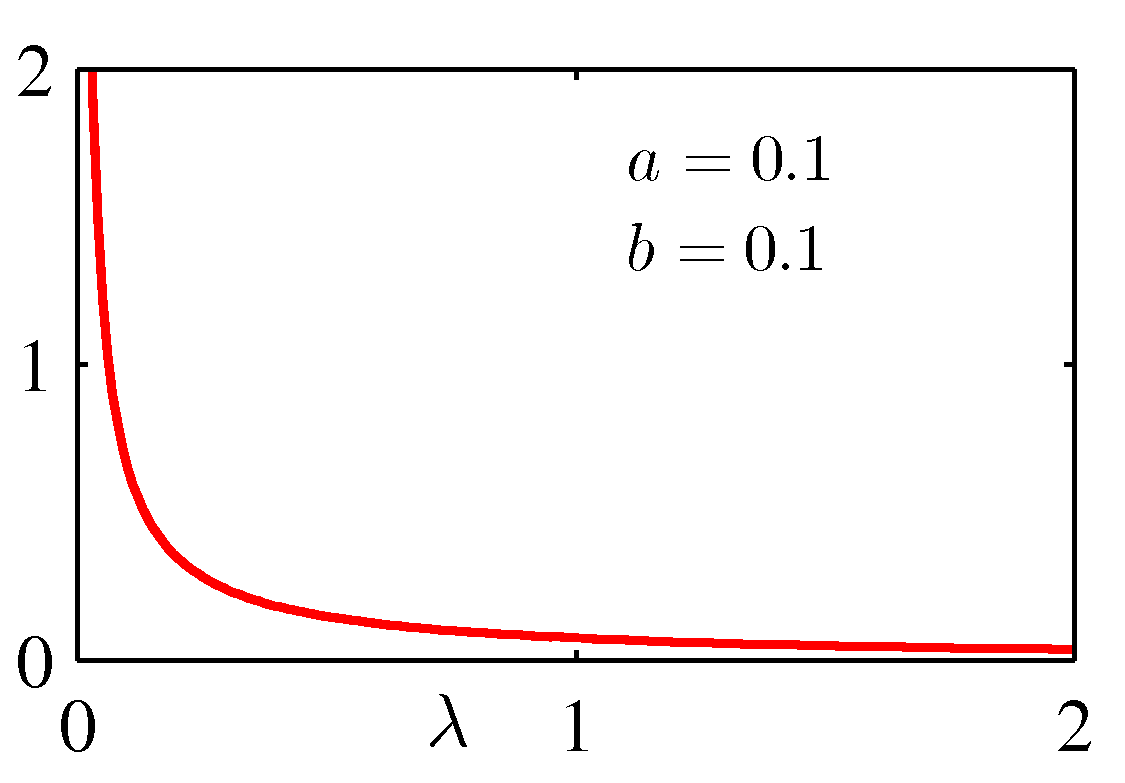
\includegraphics[scale=0.8]{Images/2-13a.png}
		\label{fig:2-13a}
		\end{minipage}
		\begin{minipage}[t]{0.3\linewidth}
		\centering
		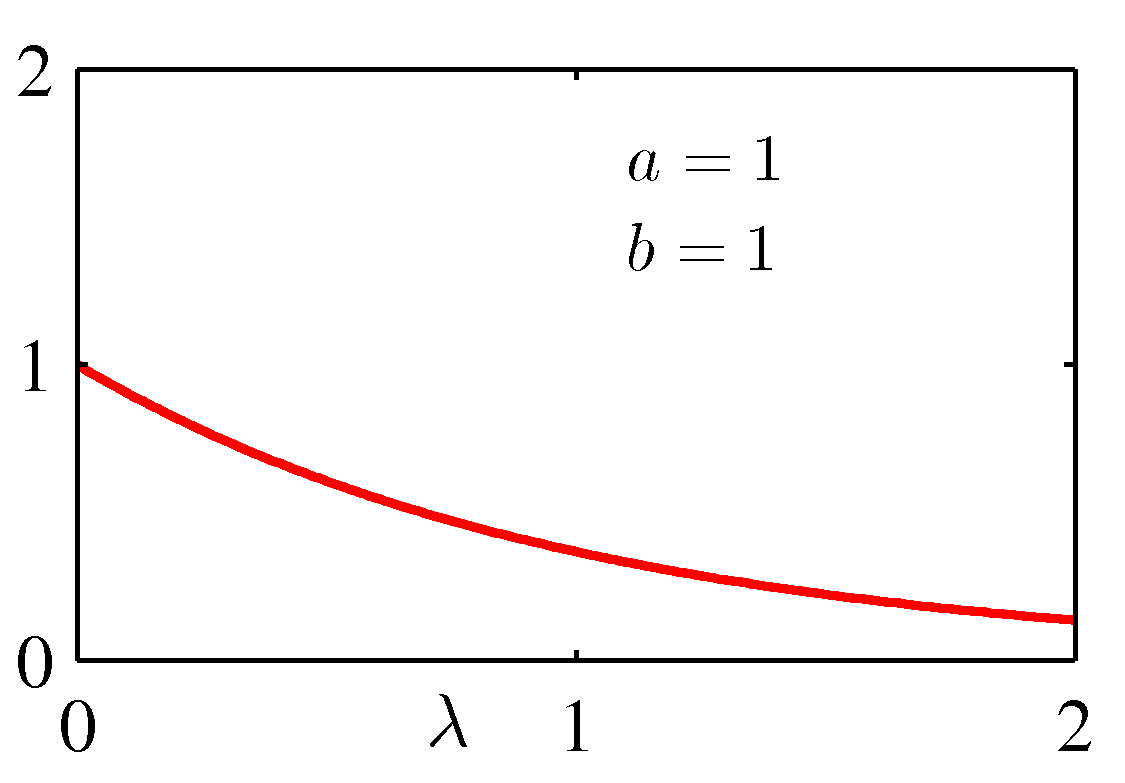
\includegraphics[scale=0.8]{Images/2-13b.png}
		\label{fig:2-13b}
		\end{minipage}
		\begin{minipage}[t]{0.3\linewidth}
		\centering
		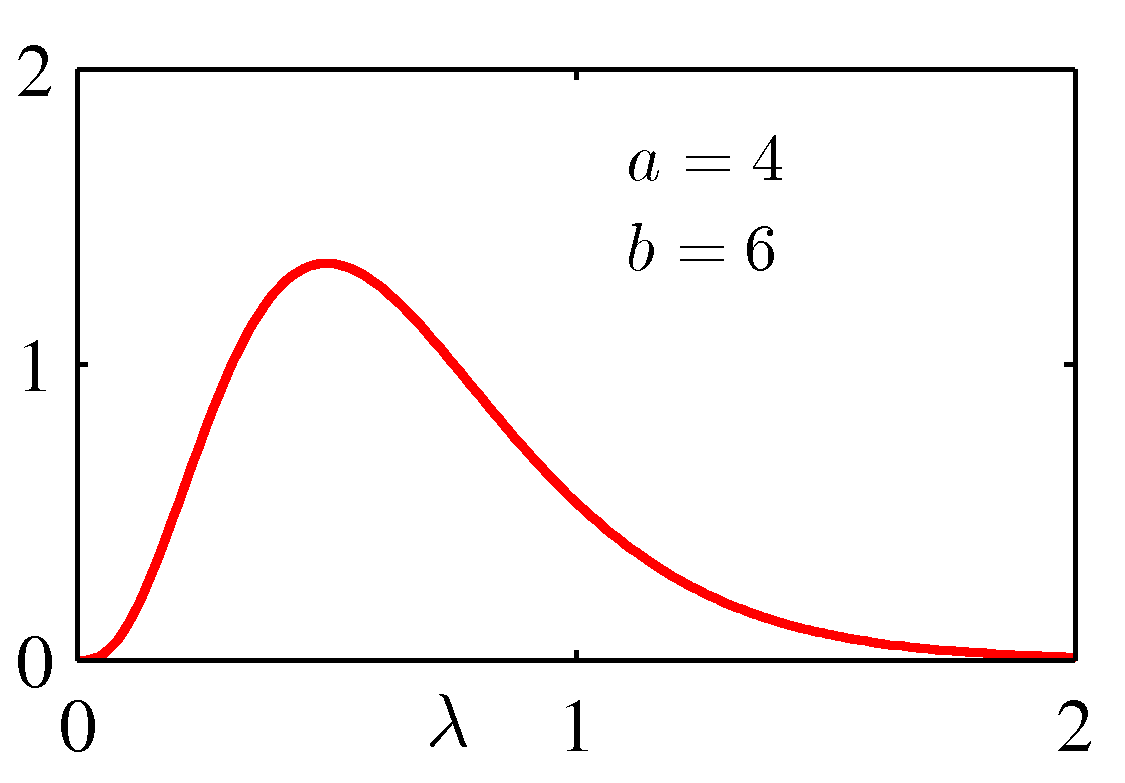
\includegraphics[scale=0.8]{Images/2-13c.png}
		\label{fig:2-13c}
		\end{minipage}
		\captionsetup{font={small}}
		\caption{根据(2.146),在参数$a$和$b$取不同值时的Gamma分布$\mathrm{Gam}(\lambda|a,b)$的图像。}
	\end{figure}
	\\
	\indent Gamma分布的均值和方差分别为\textcolor{red}{\textbf{——习题 2.42}}
	\begin{align}
		\mathbb{E}[\lambda] &= \frac{a}{b}\\
		\mathrm{var}[\lambda] &=\frac{a}{b^2}
	\end{align}
	\indent 假设有一个先验分布$\mathrm{Gam}(\lambda|a_0,b_0)$。乘上一个似然函数(2.145),就可以得到后验分布
	\begin{equation}
		p(\lambda|\sfx)\propto\lambda^{a_0-1}\lambda^{N/2}\exp\left\{-b_0\lambda-\frac{\lambda}{2}\sum_{n=1}^N(x_n-\mu)^2\right\}
	\end{equation}
	我们可以认为这是一个形式为$\mathrm{Gam}(\lambda|a_N,b_N)$的Gamma分布,其中
	\begin{align}
		a_N&=a_0+\frac{N}{2} \\
		b_N&=b_0+\frac{1}{2}\sum_{n=1}^N(x_n-\mu)^2=b_0+\frac{N}{2}\sigma_{\mathrm{ML}}^2
	\end{align}
	其中$\sigma_{\mathrm{ML}}^2$是方差的最大似然估计。注意到(2.149)中没有必要一直盯着先验和似然函数中的归一化常数,因为如果需要的话,直接把(2.146)中的Gamma函数进行归一化就可以了。\\
	\indent 从(2.150)可以看出这$N$组数据会让系数$a$的值以$N/2$的速度上升。所以可以把先验中的参数$a_0$解释为$2a_0$个“有效的”先验观测。类似地,从(2.151)可以看出,这$N$组数据对参数$b$造成的影响是$N\sigma_{\mathrm{ML}}^2/2$,其中$\sigma_{\mathrm{ML}}^2$为方差,于是就可以将参数$b_0$解释为,$2a_0$个“有效”先验观测的方差为$2b_0/(2a_0)=b_0/a_0$。回想一下,我们曾经对狄利克雷先验做过类似的解释。\textcolor{red}{\textbf{——第2.2节}}\ 这些分布都属于指数族,我们将看到,在指数型分布族中,根据有效的假想数据对共轭先验的解释是通用的。\\
	\indent 如果不使用精度,利用方差本身进行推导也是可以的。在这种情况下的共轭先验称为逆Gamma分布,但我们不会过多讨论它,因为使用精度进行推导要简单很多。\\
	\indent 现在假设均值和精度都是未知的。为了求取共轭先验,考虑到似然函数对$\mu$和$\lambda$的依赖:
	\begin{equation}
	\begin{split}
		&p(\sfx|\mu,\lambda)=\prod_{n=1}^{N}(\frac{\lambda}{2\pi})^{1/2}\exp\left\{-\frac{\lambda}{2}(x_n-\mu)^2\right\} \\
		&\propto \left[\lambda^{1/2}\exp(-\frac{\lambda\mu^2}{2})\right]^N \exp\left\{\lambda\mu\sum_{n=1}^Nx_n - \frac{\lambda}{2}\sum_{n=1}^Nx_n^2\right\}
	\end{split}
	\end{equation}
	我们想要确定一个先验分布$p(\mu,\lambda)$,这个先验分布对$\mu$和$\lambda$的依赖应该与似然函数具有相同的形式,也就是
	\begin{equation}
	\begin{split}
		&p(\mu,\lambda) \propto \left[\lambda^{1/2}\exp(-\frac{\lambda\mu^2}{2})\right]^\beta \exp\{c\lambda\mu-d\lambda\}\\
		&=\exp\left\{-\frac{\beta\lambda}{2}(\mu-c/\beta)^2\right\}\lambda^{\beta/2}\exp\left\{-{d-\frac{c^2}{2\beta}}\lambda\right\}
	\end{split}
	\end{equation}
	其中$c,d$和$\beta$都是常数。既然我们一直有$p(\mu,\lambda)=p(\mu|\lambda)p(\lambda)$,那么就可以对$p(\mu|\lambda)$和$p(\lambda)$做做文章。特别地,$p(\mu|\lambda)$其实是一个高斯分布,其精度是$\lambda$的线性函数;而$p(\lambda)$是一个Gamma分布,于是归一化先验的形式为
	\begin{equation}
		p(\mu,\lambda)=\mathcal{N}(\mu|\mu_0,(\beta\lambda)^{-1})\mathrm{Gam}(\lambda|a,b)
	\end{equation}
	其中我们定义了新的常数,$\mu_0=c/ \beta$,$a=(1+\beta)/2$,$b=d-c^2/2\beta$。(2.154)中的分布称为正态Gamma分布或者高斯Gamma分布,图像如图2.14所示。需要注意的是,这不仅仅是一个关于$\lambda$的Gamma先验与一个与之独立的关于$\mu$的高斯先验的乘积,因为$\mu$的精度是关于$\lambda$的线性函数。即使我们选择了使得$\mu$与$\lambda$相互独立的先验,在后验分布中,$\mu$的精度也会和$\lambda$不可避免地扯上关系。
	\begin{figure}[ht]
		\centering
		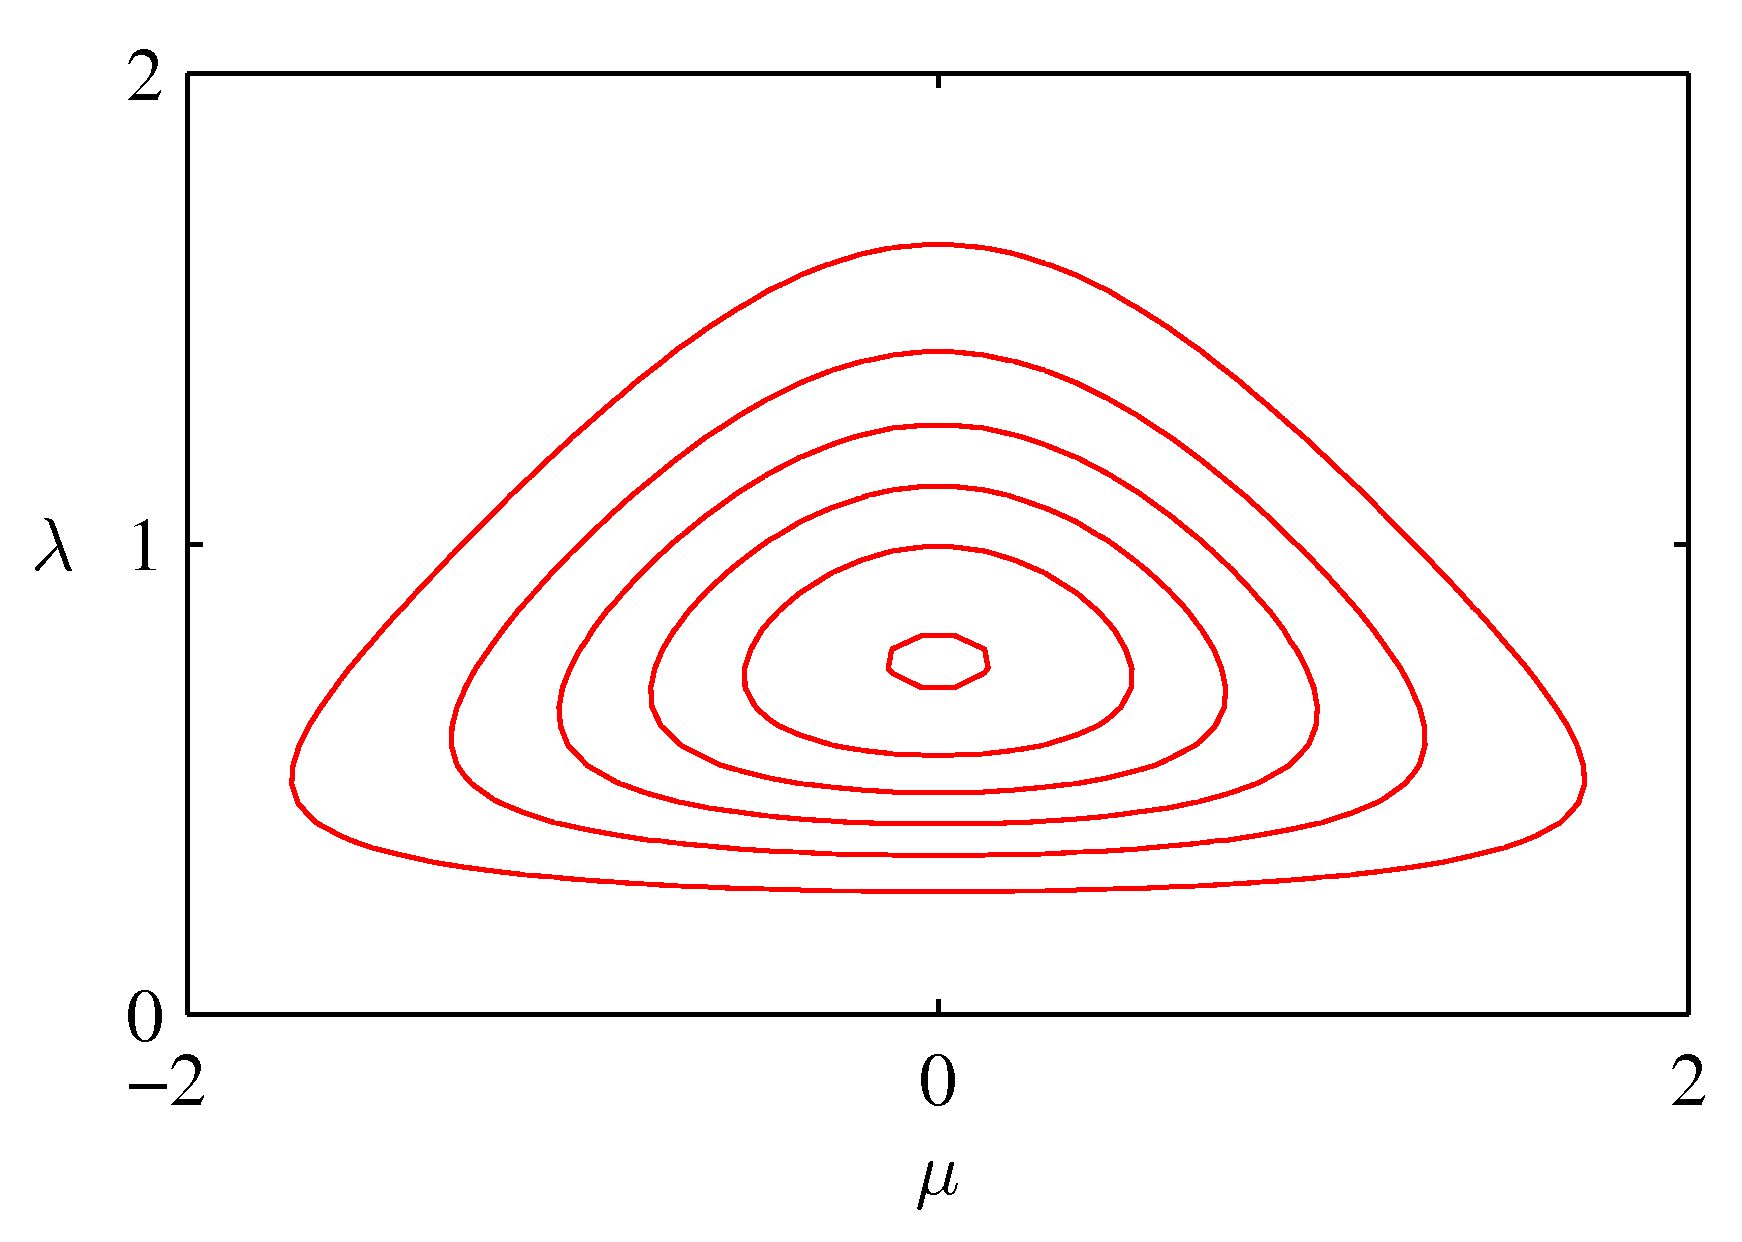
\includegraphics[scale=0.8]{Images/2-14.png}
		\captionsetup{font={small}}
		\caption{参数为$\mu_0=0,\beta=2,a=5,b=6$的正态Gamma分布(2.154)的轮廓线。}
		\label{fig:2-14}
	\end{figure}
	\\
	\indent 对于$D$维变量$\bx$多元高斯分布$\mathcal{N}(\bx|\bfMu,\bfLambda^{-1})$,假设精度已知,那么其均值$\bfMu$的共轭先验就又是一个高斯分布。对于已知均值但未知精度矩阵$\bfLambda$的情况,其共轭先验为维希特分布(Wishart distribution),表达式为\textcolor{red}{\textbf{——习题 2.45}}
	\begin{equation}
		\mathcal{W}(\bfLambda|\mathbf{W},\nu)=B|\bfLambda|^{(\nu-D-1)/2}\exp\left(-\frac{1}{2}\mathrm{Tr}(\mathbf{W}^{-1}\bfLambda)\right)
	\end{equation}
	其中$\nu$【译者注:这是希腊字母nu】称为分布的自由度,$\mathbf{W}$为$D\times D$维的矩阵,$\mathrm{Tr(\cdot)}$表示迹。归一化常数$B$为
	\begin{equation}
		B(\mathbf{W},\nu)=|\mathbf{W}|^{-\nu/2}\left(2^{\nu D/2}\pi^{D(D-1)/4}\prod_{i=1}^D\Gamma\left(\frac{\nu+1-i}{2}\right)\right)^{-1}
	\end{equation}
	和上次一样,关于协方差矩阵本身,而非精度矩阵,定义共轭先验也是可以的,那样得到的就是逆维希特分布,但我们还是不讨论它。如果均值和精度都是未知的,那么通过与一元变量情况类似的办法,可以得到共轭先验
	\begin{equation}
		p(\bfMu,\bfLambda|\bfMu_0,\beta,\mathbf{W},\nu)=\mathcal{N}(\bfMu|\bfMu_0,(\beta\bfLambda))^{-1}\mathcal{W}(\bfLambda|\mathbf{W},\nu)
	\end{equation}
	这个先验称为正态维希特分布或者高斯-维希特分布。
	}
	\subsection{学生t分布}
	\textnormal{
	我们已经看到,高斯分布精度的共轭分布是Gamma分布。对于一个一元高斯分布$\mathcal{N}(x|\mu,\tau^{-1})$和一个Gamma先验$\mathrm{Gam}(\tau|a,b)$,对精度进行积分,可以得到$x$的边缘分布\textcolor{red}{\textbf{——习题 2.46}}
	\begin{equation}
	\begin{split}
		p(x|\mu,a,b)&=\int_0^{\infty}\mathcal{N}(x|\mu,\tau^{-1})\mathrm{Gam}(\tau|a,b)\ \mathrm{d}\tau \\
		&= \int_0^{\infty}\frac{b^a e^{(-b\tau)}\tau^{a-1}}{\Gamma(a)} \left(\frac{\tau}{2\pi}\right)^{1/2}\exp\left\{-\frac{\tau}{2}(x-\mu)^2\right\}\ \mathrm{d}\tau \\
		&= \frac{b^a}{\Gamma(a)}\left(\frac{1}{2\pi}\right)^{1/2}\left[b+\frac{(x-\mu)^2}{2}\right]^{-a-1/2}\Gamma(a+1/2)
	\end{split}
	\end{equation}
	其中我们进行了变量替换$z=\tau[b+(x-\mu)^2/2]$。根据习惯定义了新的常数$\nu=2a$和$\lambda=a/b$,于是分布$p(x|\mu,a,b)$的形式改写为
	\begin{equation}
		\mathrm{St}(x|\mu,\lambda,\nu)=\frac{\Gamma(\nu /2 + 1/2)}{\nu /2}\left(\frac{\lambda}{\pi \nu}\right)^{1/2}\left[1+\frac{\lambda(x-\nu)^2}{\nu}\right]^{-\nu /2 - 1/2}
	\end{equation}
	这就是学生t分布(Student’s t-distribution)。参数$\lambda$有时被称为t分布的精度,尽管这并非严格等价于方差的逆。参数$\nu$称为自由度,其影响如图2.15所示。对于$\nu=1$的情况,t分布退化为柯西分布(Cauchy distribution),如果取极限$\nu \rightarrow \infty$,那么t分布$\mathrm{St}(x|\mu,\lambda,\nu)$就会变成一个高斯分布$\mathcal{N}(x|\mu,\lambda^{-1})$,均值为$\mu$,精度为$\lambda$。\textcolor{red}{\textbf{——习题 2.47}}
	\begin{figure}[ht]
		\centering
		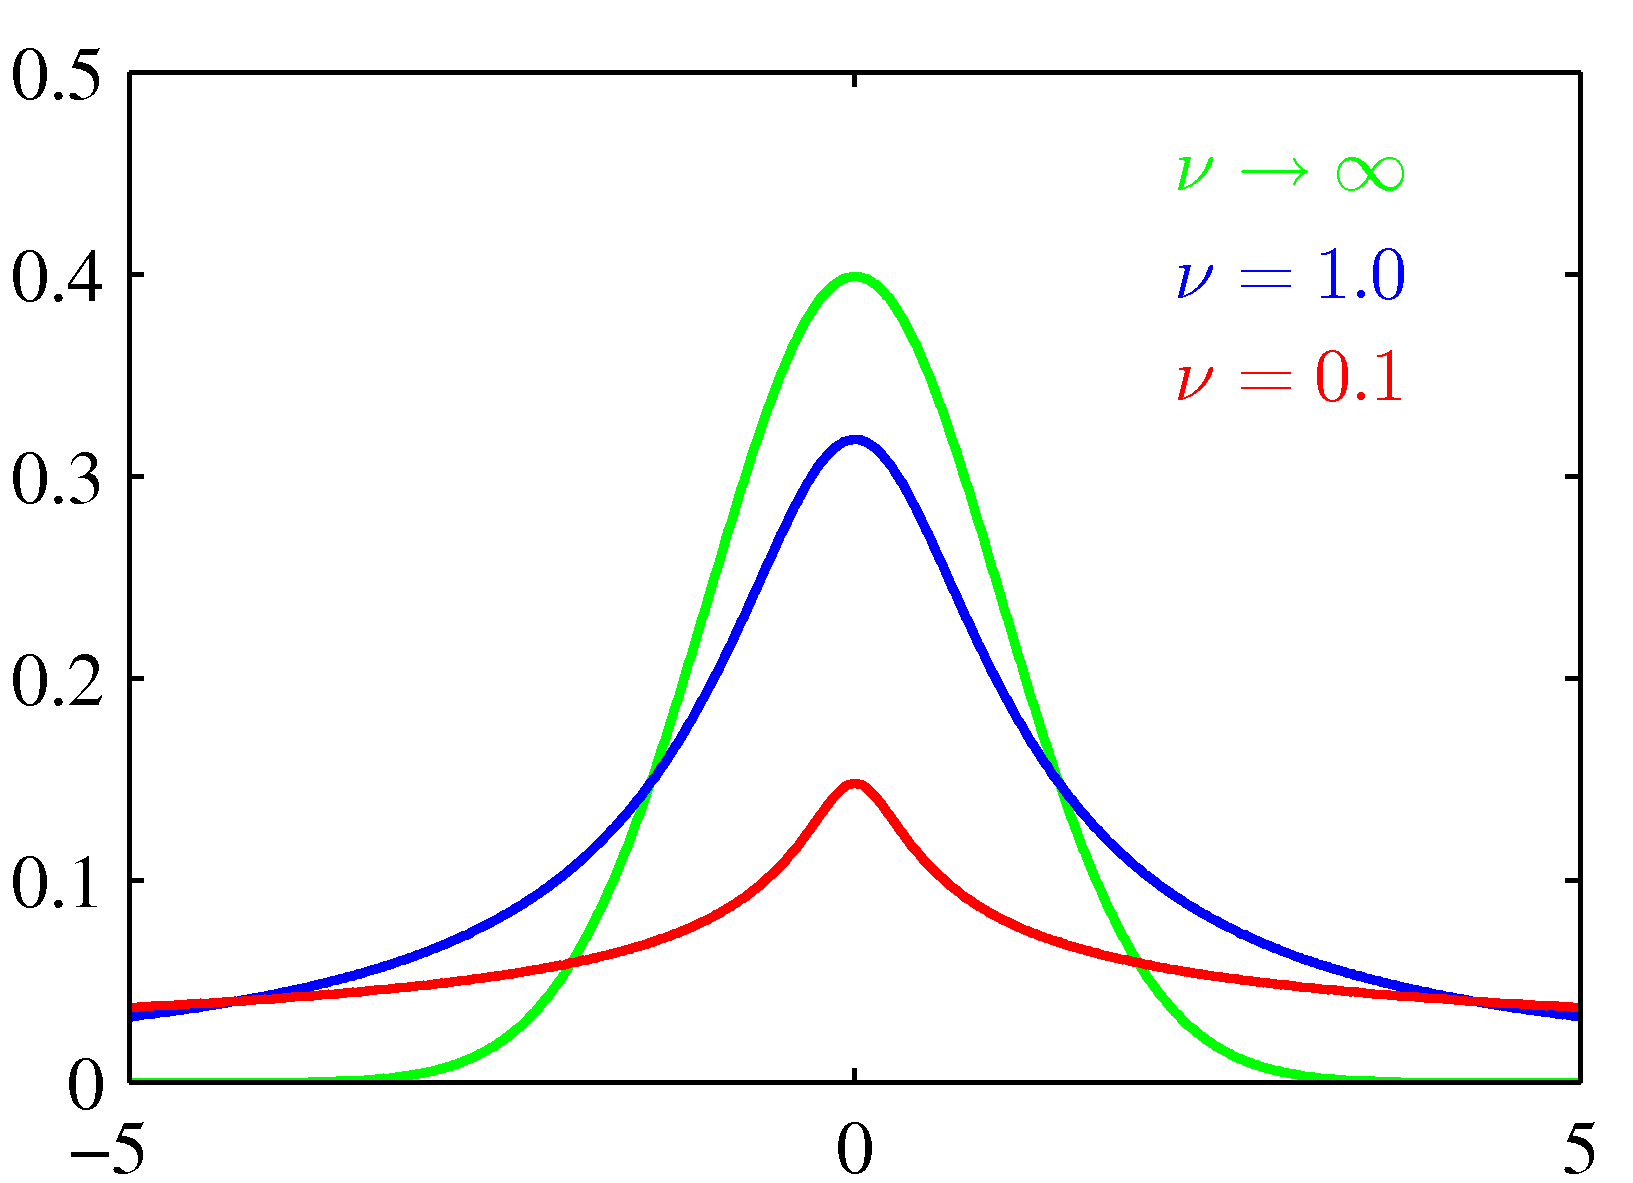
\includegraphics[scale=0.8]{Images/2-15.png}
		\captionsetup{font={small}}
		\caption{学生t分布(2.159)的图像,其中$\mu=0$,$\lambda=1$,$\nu$在不同取值时曲线也随之变化。当$\nu \rightarrow \infty$时,分布变成均值为$\mu$,精度为$\lambda$的高斯分布。}
		\label{fig:2-15}
	\end{figure}
	\\
	\indent 根据(2.158),可以看出学生t分布实质上是将无穷多个具有相同均值,但精度不同的高斯分布叠加起来得到的。这可以通过无限的高斯混合模型来解释(高斯混合模型将在第2.3.9节中进行介绍)。如图2.15所示,所得到的分布与高斯分布相比,“拖尾”要更长。这个特点使t分布具备了鲁棒性这一重要特性,与高斯分布相比,对于异常数据的敏感性要更低。t分布的鲁棒性如图2.16所示。
	\begin{figure}[ht]
		\begin{minipage}[t]{0.5\linewidth}
		\centering
		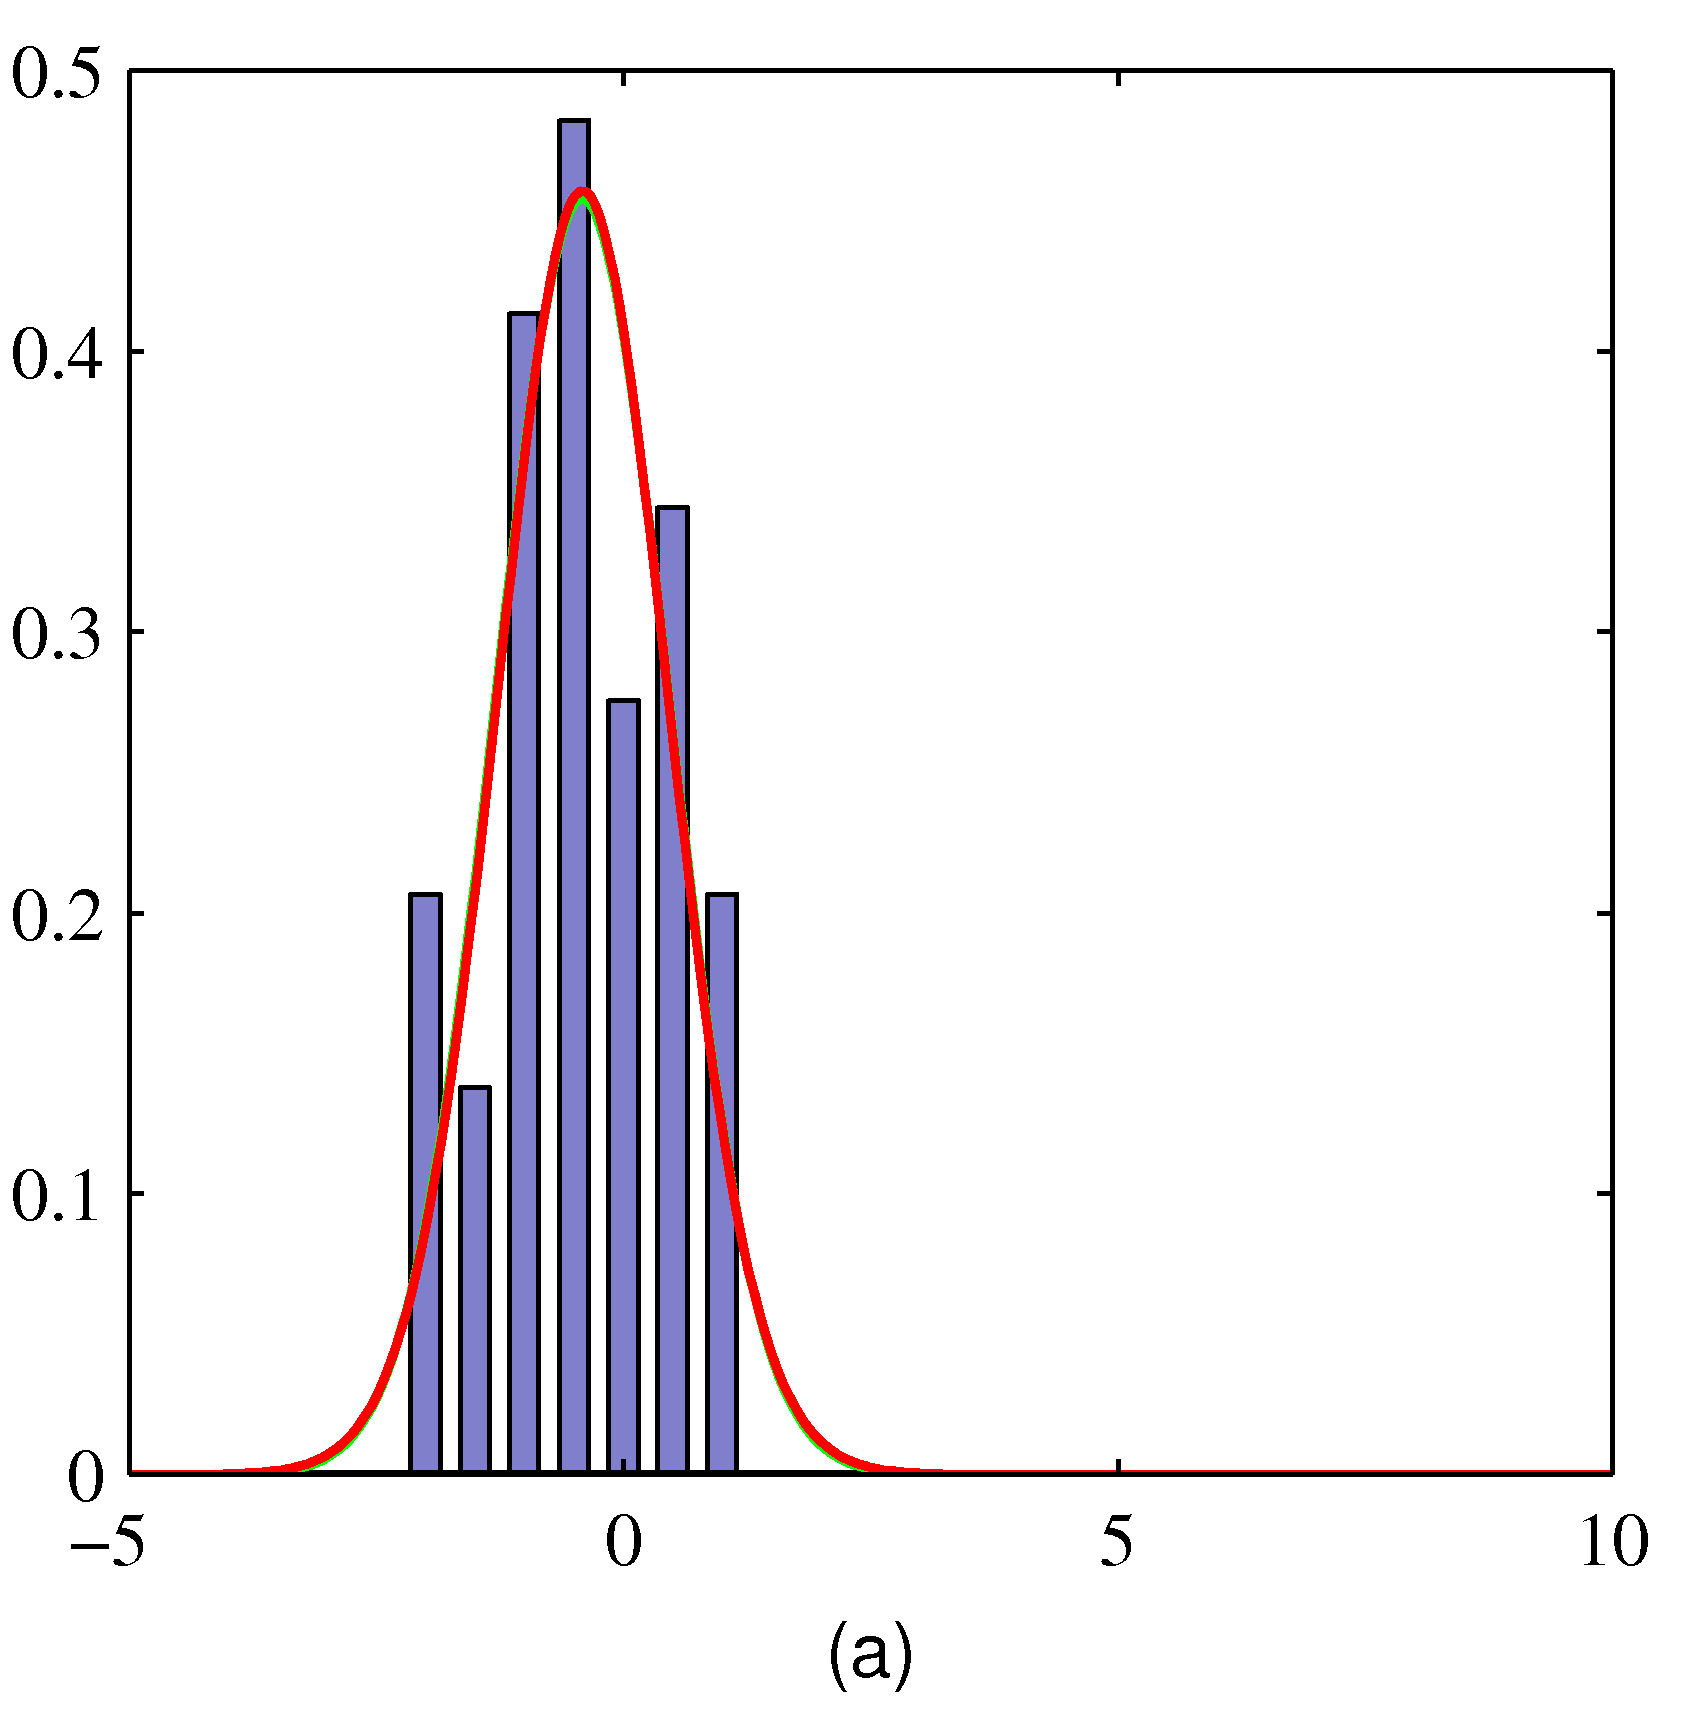
\includegraphics[scale=0.8]{Images/2-16a.png}
		\label{fig:2-16a}
		\end{minipage}
		\begin{minipage}[t]{0.5\linewidth}
		\centering
		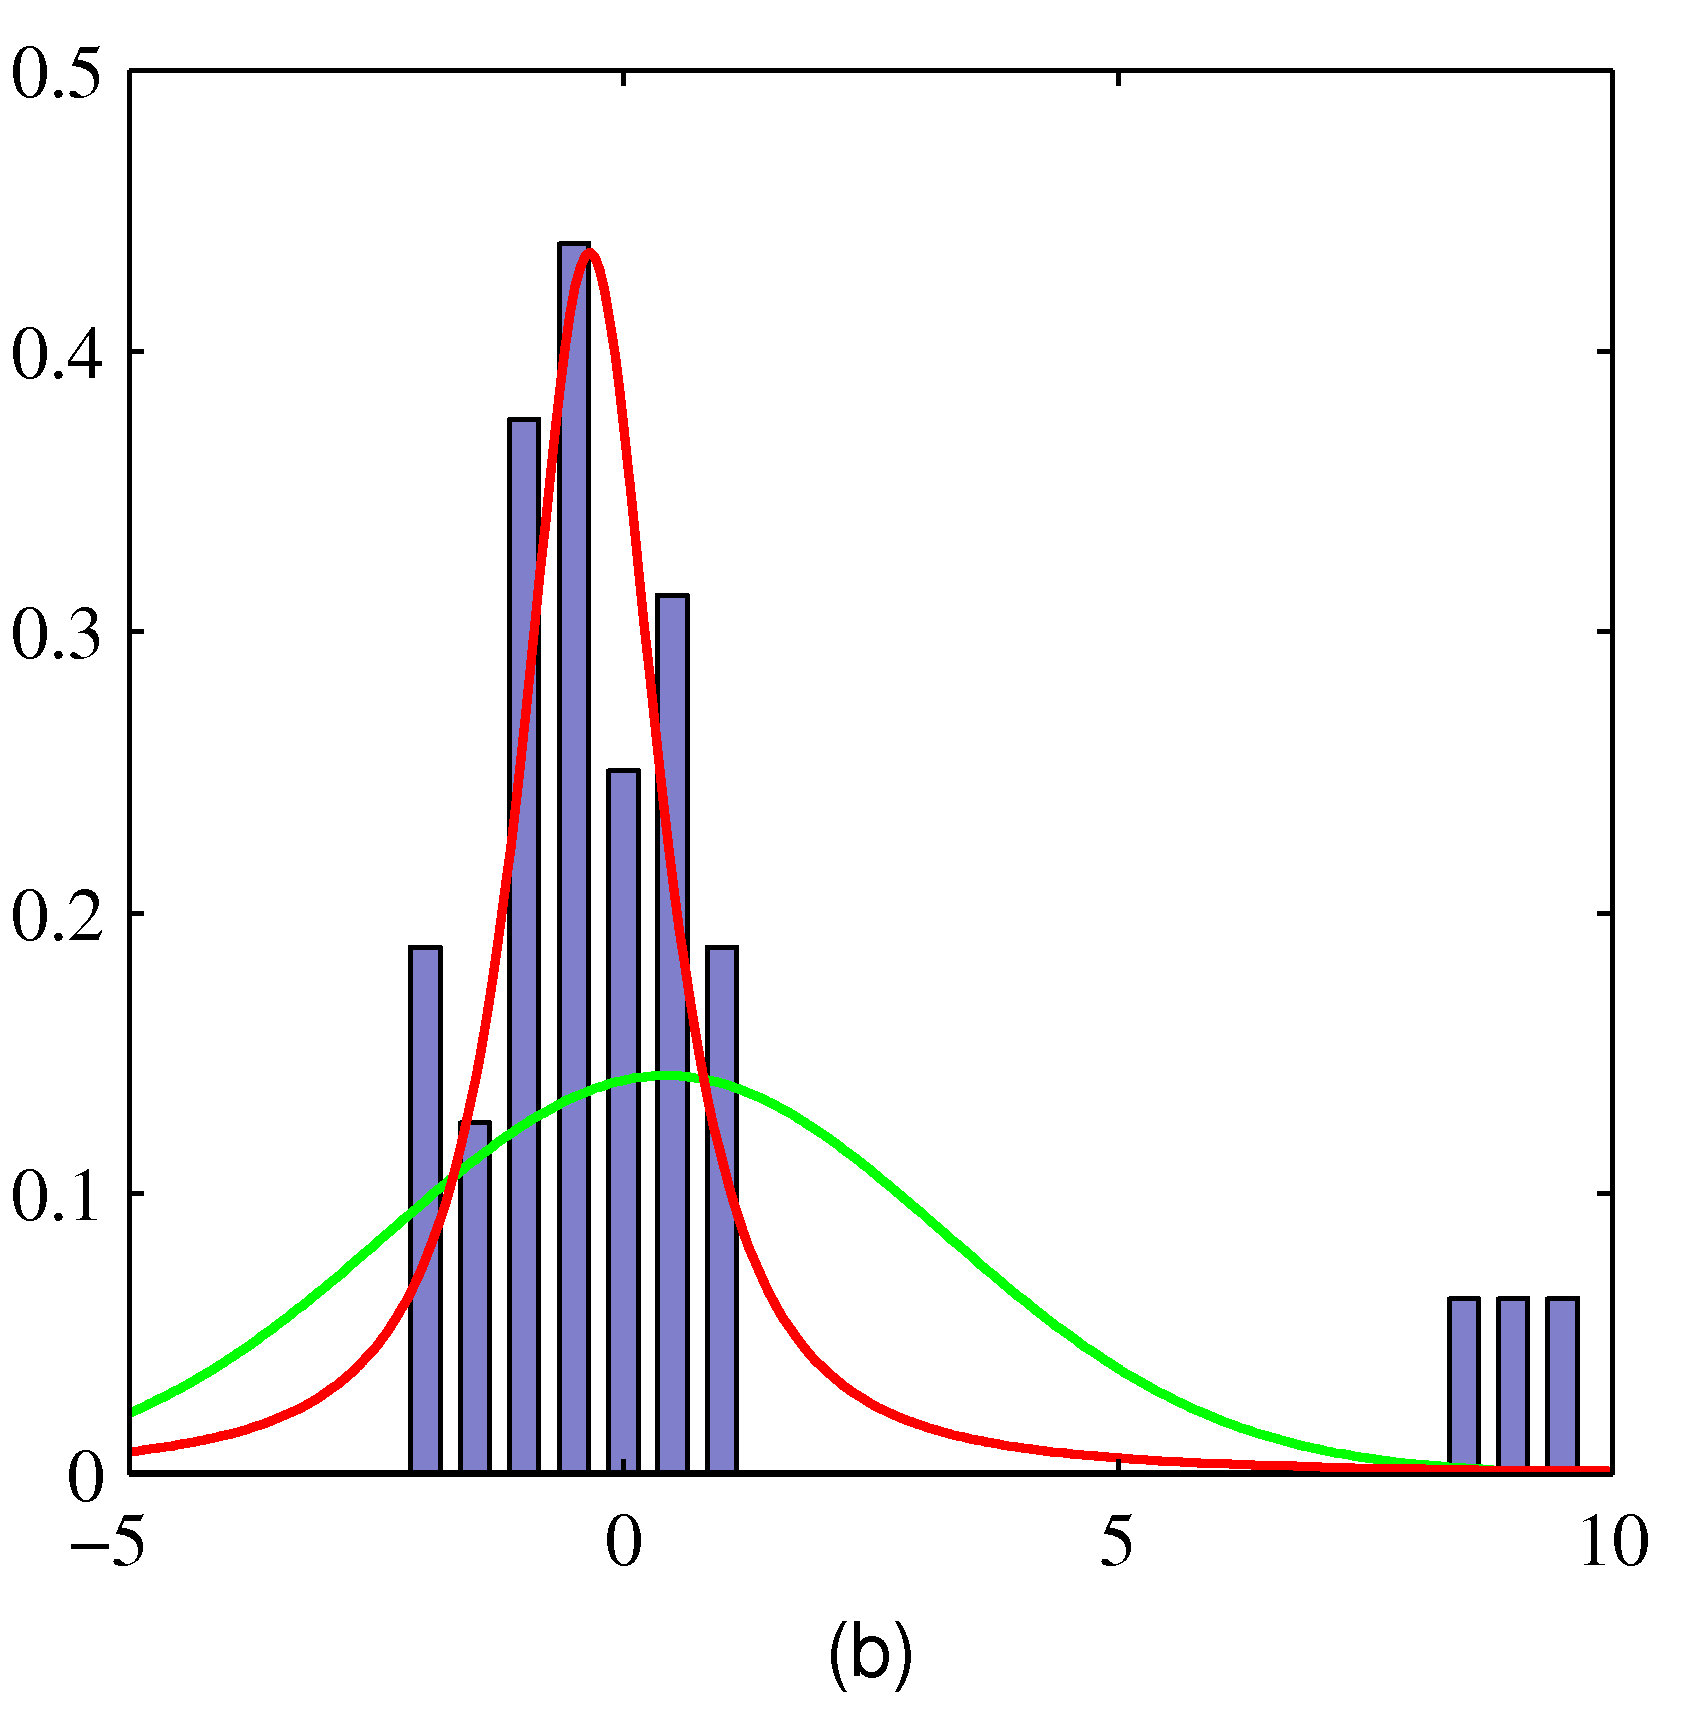
\includegraphics[scale=0.8]{Images/2-16b.png}
		\label{fig:2-16b}
		\end{minipage}
		\captionsetup{font={small}}
		\caption{学生t分布与高斯分布鲁棒性的比较。(a)为从高斯分布中取出30个数据点绘制的直方图分布。红色曲线为利用最大似然拟合得到的t分布曲线,绿色曲线为利用最大似然拟合得到的高斯分布曲线,但基本上完全被红色曲线盖住了。因为t分布包含了高斯分布——高斯分布是t分布的一种特殊情况——所以给出了与高斯分布几乎相同的解;(b)是在相同的数据集中加上了3个异常数据的结果,高斯分布明显受到了强烈的影响,但t分布几乎没有受到影响。}
	\end{figure}
	\\
	\indent 需要注意的是,t分布的最大似然解可以通过期望最大化算法(EM算法)来求取。\textcolor{red}{\textbf{——习题 12.24}}\ 在这里我们先看一下,一小撮异常数据对t分布的影响比对高斯分布的影响要小得多。异常值在实际应用中一定是存在的,既可能是因为生成数据的分布是重尾分布,也可能仅仅是因为数据的错误标注,总之异常数据很是烦人。对于回归问题而言,鲁棒性是相当重要的性质。不出意料,回归的最小二乘法并没有很好的鲁棒性,因为它对应的是(条件)高斯分布下的最大似然。通过在类似t分布这样的重尾分布中建立回归模型,我们可以得到一个鲁棒性更好的模型。\\
	\indent 回到(2.158),令$\nu = 2a, \lambda=a/b, \eta=\tau b /a$,那么t分布就可以写成
	\begin{equation}
		\mathrm{St}(x|\mu,\lambda,\nu)=\int_0^{\infty}\mathcal{N}(x|\mu,(\eta\lambda)^{-1})\mathrm{Gam}(\eta|\nu/2,\nu/2)\ \mathrm{d}\eta
	\end{equation}
	我们可以将它推广到多元高斯分布$\mathcal{N}(\bx|\bfMu,\bfLambda)$来确定多元学生t分布:
	\begin{equation}
		\mathrm{St}(\bx|\bfMu, \bfLambda, \nu) = \int_0^{\infty} \mathcal{N}(\bx|\bfMu,(\eta\bfLambda)^{-1})\mathrm{Gam}(\eta|\nu/2,\nu/2)\ \mathrm{d}\eta
	\end{equation}
	利用与一元情况一样的手段,可以处理这个积分,得到\textcolor{red}{\textbf{——习题 2.48}}
	\begin{equation}
		\mathrm{St}(\bx|\bfMu, \bfLambda, \nu)=\frac{\Gamma(D/2+\nu/2)}{\Gamma(\nu/2)}\frac{|\bfLambda|^{1/2}}{(\pi\nu)^{D/2}}\left[1+\frac{\Delta^2}{\nu}\right]^{-D/2-\nu/2}
	\end{equation}
	其中$D$为$\bx$的维数,$\Delta^2$为Mahalanobis距离的平方:
	\begin{equation}
		\Delta^2 = (\bx - \bfMu)^{\rmT}\bfLambda(\bx-\bfMu)
	\end{equation}
	这就是多元形式的学生t分布,而且满足如下性质:\textcolor{red}{\textbf{——习题 2.49}}
	\begin{align}
		\mathbb{E}[\bx]&=\bfMu, \mathrm{if}\ \nu>1 \\
		\mathrm{cov}[\bx] &= \frac{\nu}{\nu-2}\bfLambda^{-1}, \mathrm{if}\ \nu>2 \\
		\mathrm{mode}[\bx]&=\bfMu
	\end{align}
	这些性质与一元的情况是一一对应的。
	}
	\subsection{周期变量}
	\textnormal{
	尽管高斯分布在实际应用中具有非凡的意义,它们自身的优点就很多,而且还能充当复杂概率模型的重要基础。不过,高斯分布终究还是有力不从心的时候,比如对连续变量建立密度模型。在实际应用中,一个很要命的情况就是遇到周期变量。\\
	\indent 周期变量很容易举例,比如某个特定地理位置处的风向。我们可能会在几天的时间内测量风向,并利用参数分布进行总结。另一个例子是日期时间,我们可能会对超过24小时或1年这样周期的量进行建模。这样的数量使用角度(极坐标)$0 \leqslant \theta < 2\pi$进行表示比较方便。\\
	\indent 在这样的问题中,第一反应往往是选定某个方向作为原点,然后应用类似高斯分布这样的传统分布进行建模。但是,这样的方法会导致一个问题,那就是模型给出的结果对原点的选择存在很强的依赖。比如,假设在$\theta_1=1^\circ$处和$\theta_2=359^\circ$处有两组数据,使用一元的标准高斯分布进行建模。假设原点位于$0^\circ$,那么样本均值为$180^\circ$,标准差为$179^\circ$,但要是把原点设置在$180^\circ$,那么均值就是$0^\circ$,标准差就是$1^\circ$了。显然,我们需要一种更有效的办法来处理周期变量。\\
	\indent 首先来研究一下某个周期变量的观测数据$\mathcal{D}=\{\theta_1,...,\theta_N\}$的均值。从现在开始,我们默认$\theta$的单位是弧度。从之前的例子已经可以看出,简单的平均值$(\theta_1+...+\theta_N)/N$将会对原点坐标形成很强的依赖。为了找到一个不变的平均值度量,需要注意到这些数据都是单位圆上的点,于是就可以用二维单位向量$\bx_1,...,\bx_N$来表示,其中$\| \bx_n \|=1, n=1,...,N$,如图2.17所示。我们可以对向量$\{\bx_n\}$求平均值:
	\begin{equation}
		\overline{\bx}=\frac{1}{N}\sum_{n=1}^N \bx_n
	\end{equation}
	\begin{figure}[ht]
		\centering
		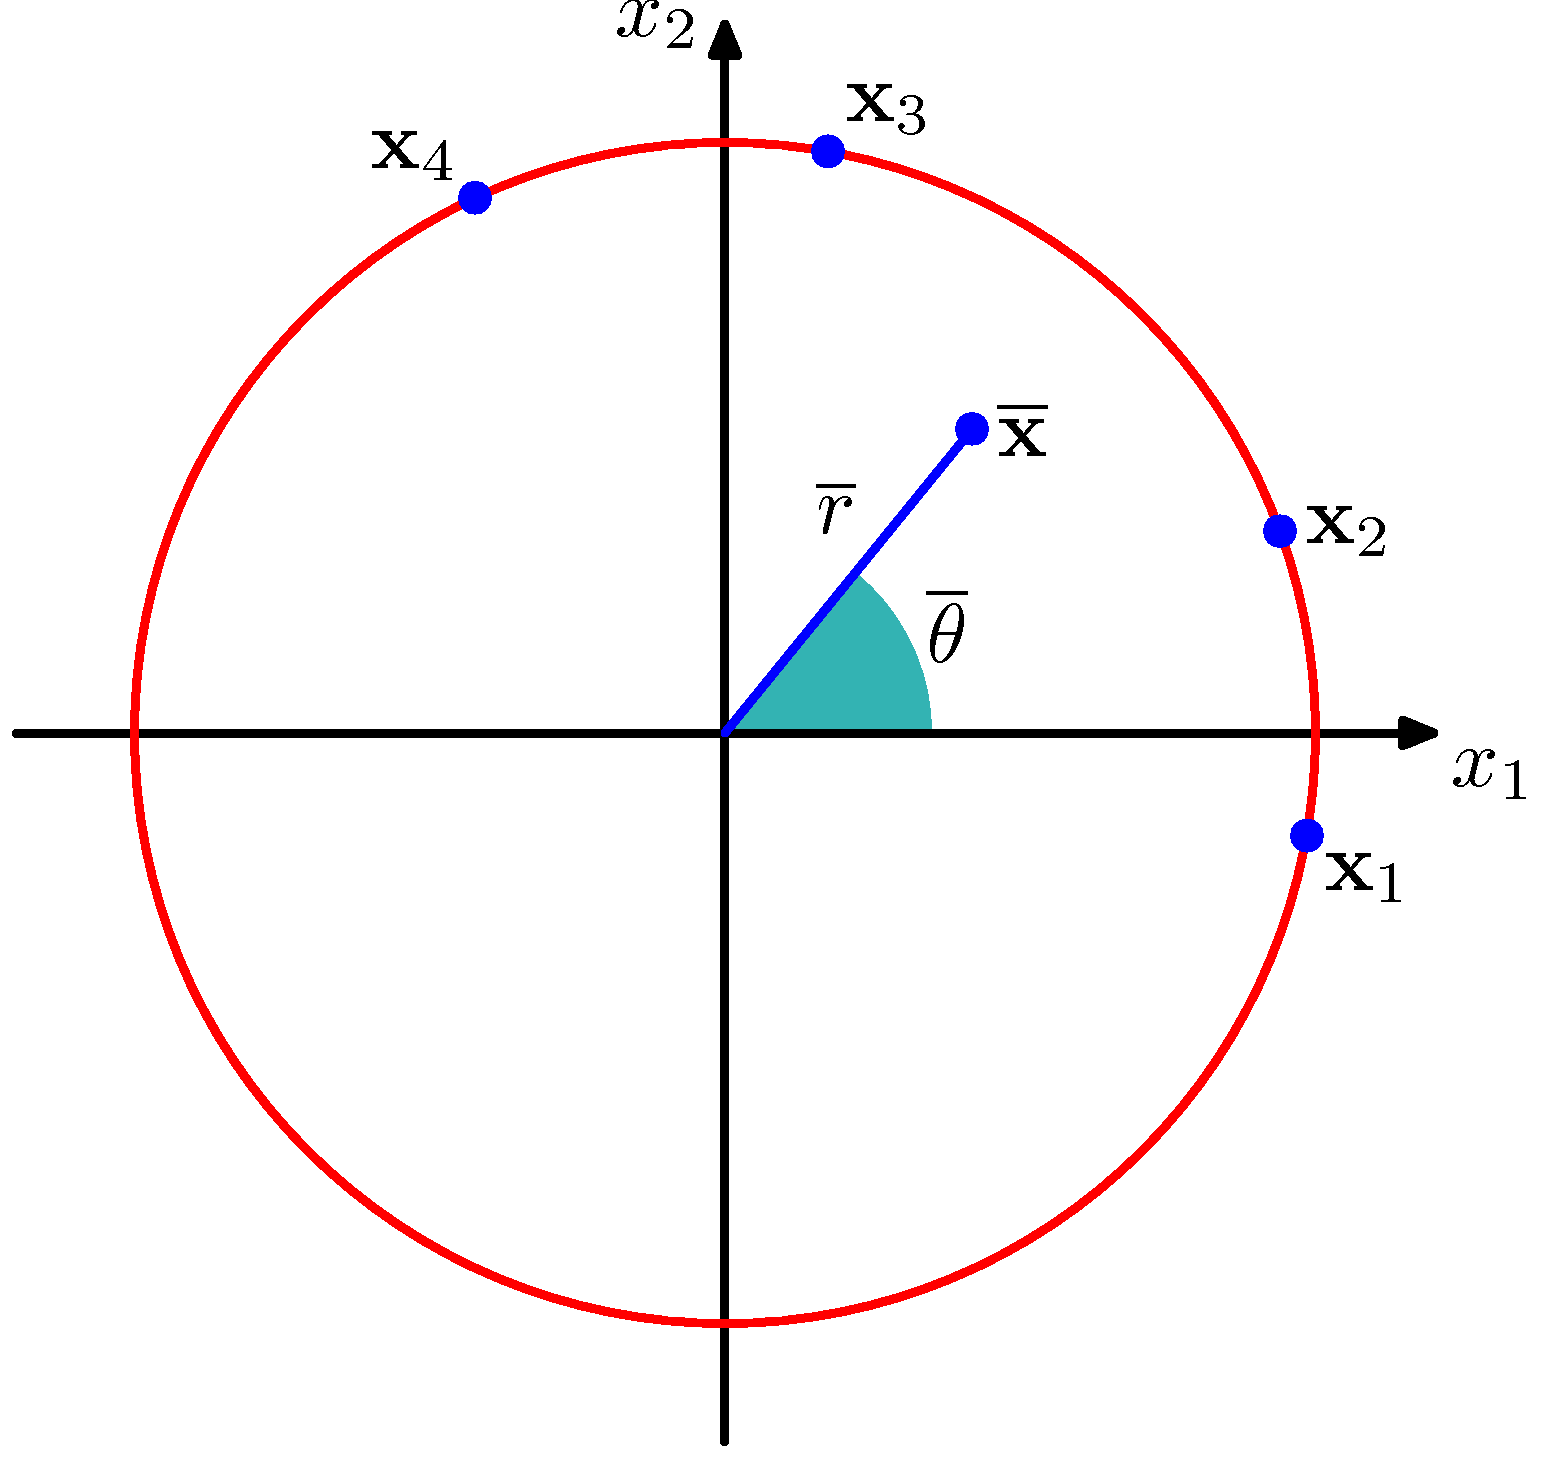
\includegraphics[scale=0.8]{Images/2-17.png}
		\captionsetup{font={small}}
		\caption{利用二维向量$\bx_n$表示周期变量$\theta_n$的示意图,所有的点都位于单位圆上。同时也标出了向量的均值$\overline{\bx}$。}
		\label{fig:2-17}
	\end{figure}
	然后求取对应的角度平均值$\overline{\theta}$。很明显,这样的定义可以确保均值的位置与角度坐标的原点无关。注意到$\overline{\bx}$一定是位于单位圆内的,那么它的笛卡尔坐标可以写成$\bx_n=(\cos \theta_n, \sin \theta_n)$,同样可以将样本均值的笛卡尔坐标写成$\overline{\bx}=(\overline{r}\cos \overline{\theta}, \overline{r}\sin \overline{\theta})$。将其代入(2.167),并令$x_1$和$x_2$对应相等,可以得到
	\begin{equation}
		\overline{x}_1=\overline{r}\cos \overline{\theta} = \frac{1}{N}\sum_{n=1}^N \cos\theta_n, \ \overline{x}_2=\overline{r}\sin \overline{\theta} = \frac{1}{N}\sum_{n=1}^N \sin\theta_n
	\end{equation}
	求其比值,并利用$\tan \theta = \sin \theta/ \cos \theta$,可以得到$\overline{\theta}$:
	\begin{equation}
		\overline{\theta}=\tan^{-1}\left\{\frac{\sum_n\sin \theta_n}{\sum_n \cos \theta_n}\right\}
	\end{equation}
	很快我们会看到这个结果是关于周期变量的适当分布的最大似然估计。\\
	\indent 现在我们研究一种高斯分布在周期变量上的推广,称为冯$\cdot$米塞斯分布(von Mises distribution)。我们对此的讨论将仅限于一元分布,尽管在任意维度的超球面上都可以找到周期分布,但更加广泛的讨论,请参见Mardia and Jupp (2000)的研究。\\
	\indent 按照以往的习惯,我们认为分布$p(\theta)$的周期为$2\pi$。任何关于$\theta$的概率密度$p(\theta)$都不能为负,积分必须为1,而且必须是周期性的。于是$p(\theta)$必须满足以下3个条件:
	\begin{align}
		p(\theta)&\geqslant 0 \\
		\int_0^{2\pi} p(\theta) \ \mathrm{d}\theta &= 1 \\
		p(\theta+2\pi)&=p(\theta)
	\end{align}
	根据(2.172),同样可以写成,对于任意整数$M$,$p(\theta+M2\pi)=p(\theta)$。\\
	\indent 我们可以通过接下来的步骤来确定一个满足这3个条件的类高斯分布。假设有一个二元变量$\bx=(x_1,x_2)$的高斯分布,均值为$\bfMu=(\mu_1,\mu_2)$,协方差矩阵为$\bfSigma=\sigma^2\mathbf{I}$,其中$\mathbf{I}$为$2 \times 2$的单位矩阵,于是
	\begin{equation}
		p(x_1,x_2)=\frac{1}{2\pi \sigma^2}\exp\left\{-\frac{(x_1-\mu_1)^2+(x_2-\mu_2)^2}{2\sigma^2}\right\}
	\end{equation}
	\begin{figure}[ht]
		\centering
		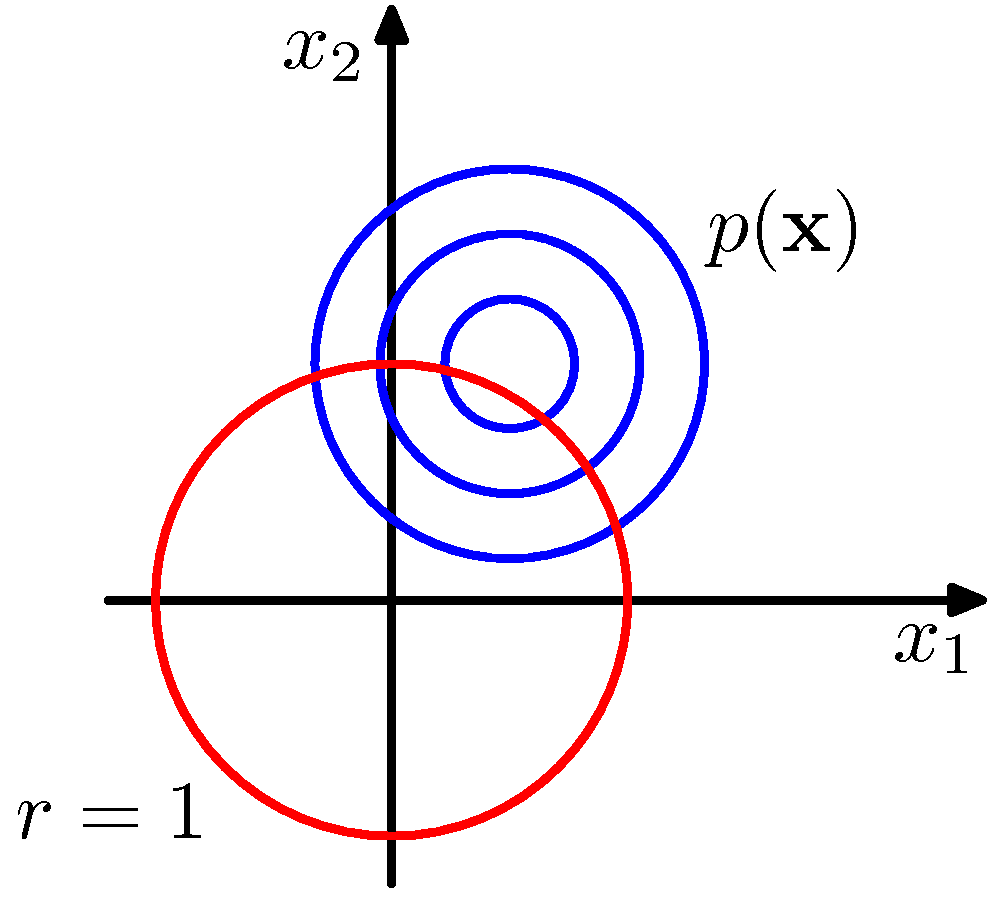
\includegraphics[scale=0.8]{Images/2-18.png}
		\captionsetup{font={small}}
		\caption{von Mises分布可以通过(2.173)中的二维高斯分布来推出,蓝色曲线表示密度轮廓线,红色曲线显示的单位圆为限制条件。}
		\label{fig:2-18}
	\end{figure}
	\\
	\indent $p(\bx)$的轮廓线是圆,如图2.18所示。现在我们认为这个分布可能的值都在一个半径固定的圆上。于是这个分布一定是周期性的,但可能不是归一化的。我们可以通过将笛卡尔坐标$(x_1,x_2)$转化为极坐标$(r,\theta)$来确定这个分布的形式,即
	\begin{equation}
		x_1=r\cos \theta, \ x_2=r \sin \theta
	\end{equation}
	同样地,均值$\bfMu$也可以写成极坐标形式
	\begin{equation}
		\mu_1 = r_0 \cos \theta_0, \ \mu_2=r_0 \sin \theta_0
	\end{equation}
	接下来我们将这些变换代入到二维高斯分布(2.173)中,由于我们只关注$\theta$,故将分布限定在单位圆上,即$r=1$。对于高斯分布的指数,可以得到
	\begin{equation}
	\begin{split}
		&-\frac{1}{2\sigma^2}\left\{(r\cos \theta-r_0 \cos \theta_0)^2 + (r\sin \theta-r_0 \sin \theta_0)^2\right\} \\
		= &-\frac{1}{2\sigma^2}\left\{1+r_0^2-2r_0\cos \theta \cos \theta_0 - 2 r_0 \sin \theta \sin \theta_0\right\} \\
		= &\ \frac{r_0}{\sigma^2}\cos(\theta-\theta_0)+\mathrm{const}
	\end{split}
	\end{equation}
	其中的“const”表示与$\theta$无关的项,我们用到了三角恒等式\textcolor{red}{\textbf{——习题 2.51}}
	\begin{align}
		\cos^2A + \sin^2A &= 1 \\
		\cos A\cos B +\sin A \sin B &= \cos(A-B)
	\end{align}
	如果定义$m=r_0/\sigma^2$,我们就可以得到在单位圆$r=1$上分布的最终表达式$p(\theta)$:
	\begin{equation}
		p(\theta|\theta_0,m)=\frac{1}{2\pi I_0(m)}\exp{m \cos (\theta-\theta_0)}
	\end{equation}
	这就是von Mises分布,或者称为循环正态(circular normal)。其中,参数$\theta_0$对应的是分布的均值,$m$则是集中参数(concentration parameter),与高斯分布的逆方差(也就是精度)是等价的。(2.179)中的归一化常数利用$I_0(m)$的形式来表达,实际上是零阶的修正第一类贝塞尔函数(Abramowitz and Stegun, 1965),其定义为
	\begin{equation}
		I_0(m)=\frac{1}{2\pi}\int_0^{2\pi}\exp\{m \cos \theta\}\ \mathrm{d}\theta
	\end{equation}
	对于较大的$m$,这个分布将变得接近高斯分布。\textcolor{red}{\textbf{——习题 2.52}}\ von Mises分布如图2.19所示,函数$I_0(m)$如图2.20所示。\\
	\indent 现在让我们研究一下von Mises分布中的参数$\theta_0$和$m$的最大似然估计。对数似然函数为
	\begin{equation}
		\ln p(\mathcal{D}|\theta_0,m)=-N\ln(2\pi)-N\ln I_0(m)+m\sum_{n=1}^N\cos (\theta_n-\theta_0)
	\end{equation}
	关于$\theta_0$求导数并令其等于0,可得
	\begin{equation}
		\sum_{n=1}^N\sin(\theta_n-\theta_0)=0
	\end{equation}
	为了解出$\theta_0$,可以用如下的三角恒等式
	\begin{equation}
		\sin(A-B)=\cos B\sin A - \cos A \sin B
	\end{equation}
	\begin{figure}[H]
		\begin{minipage}[t]{0.5\linewidth}
		\centering
		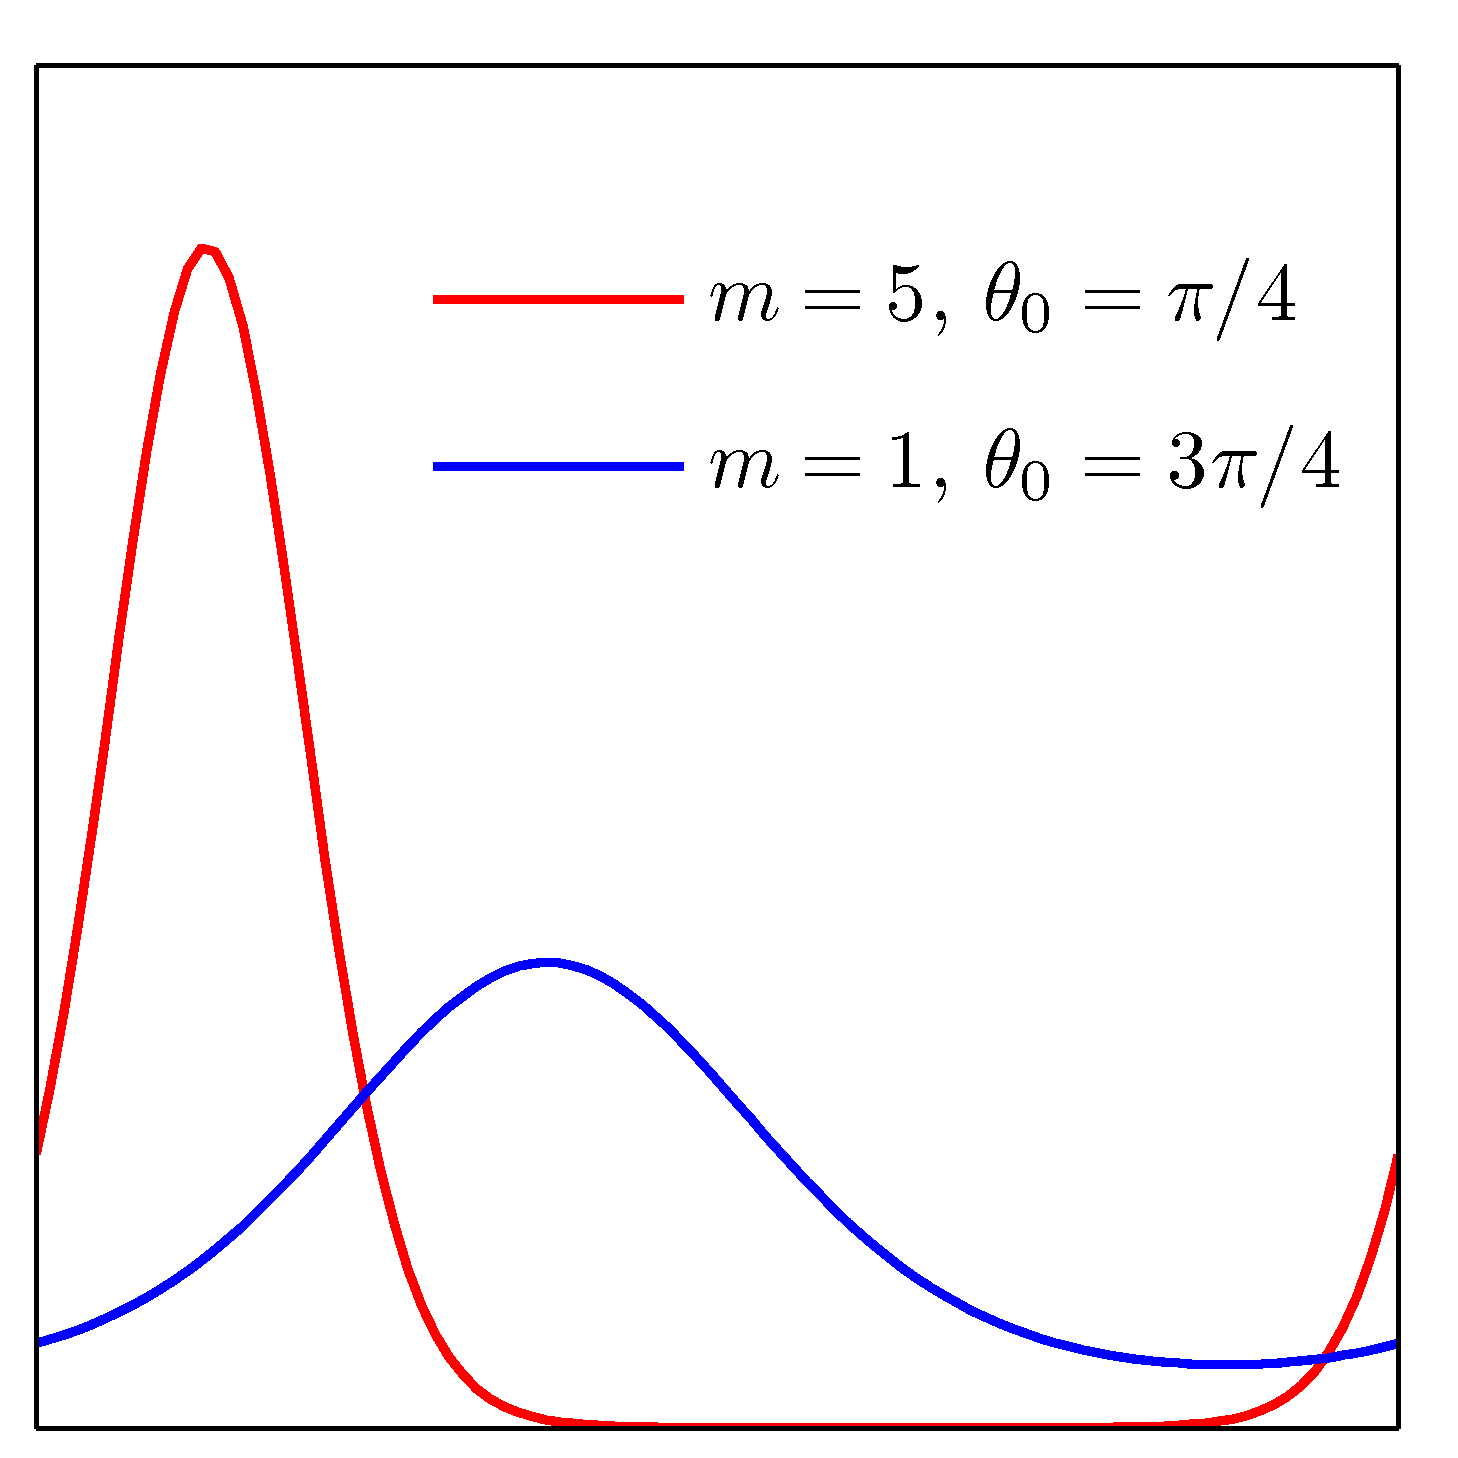
\includegraphics[scale=0.8]{Images/2-19a.png}
		\label{fig:2-19a}
		\end{minipage}
		\begin{minipage}[t]{0.5\linewidth}
		\centering
		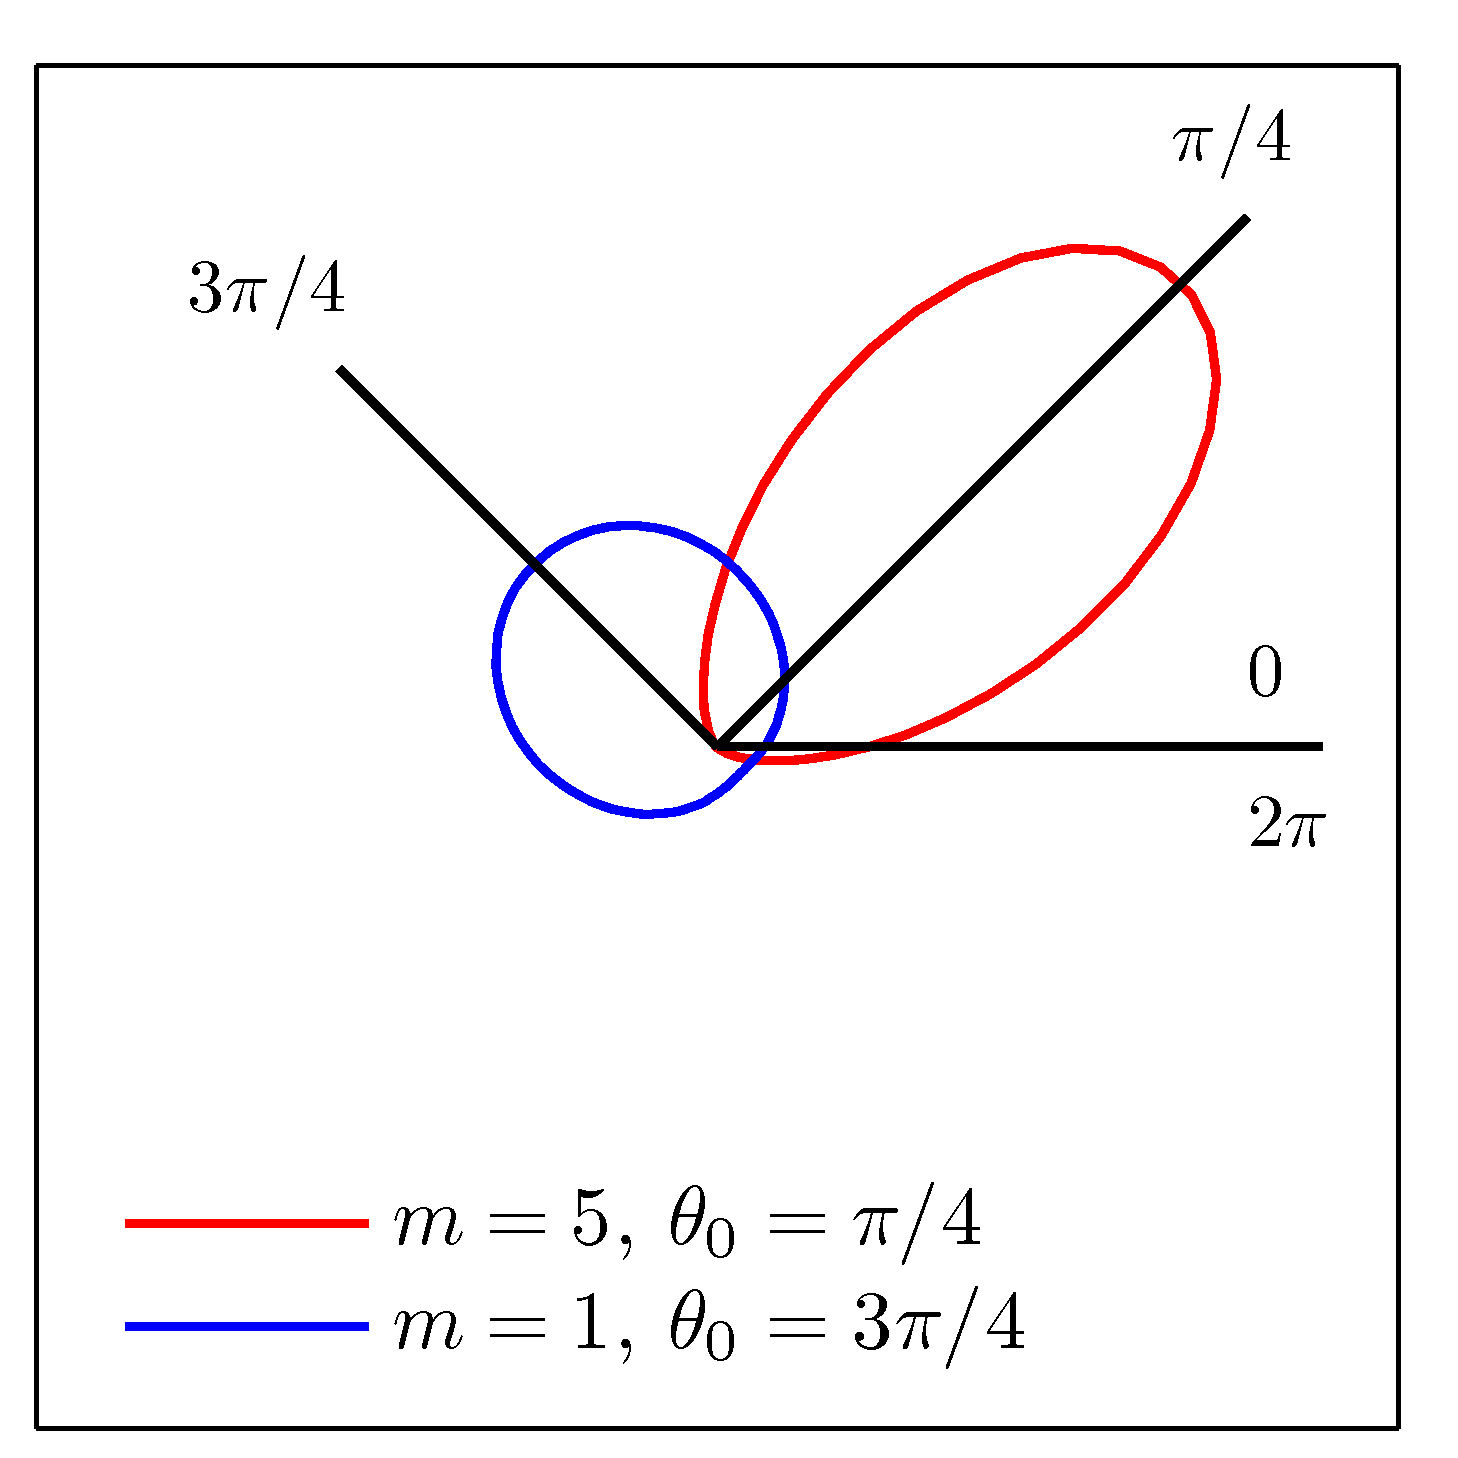
\includegraphics[scale=0.8]{Images/2-19b.png}
		\label{fig:2-19b}
		\end{minipage}
		\captionsetup{font={small}}
		\caption{在两组不同的参数值下绘制的von Mises分布,左侧为笛卡尔图,右侧为相应的极坐标图。}
		\begin{minipage}[t]{0.5\linewidth}
		\centering
		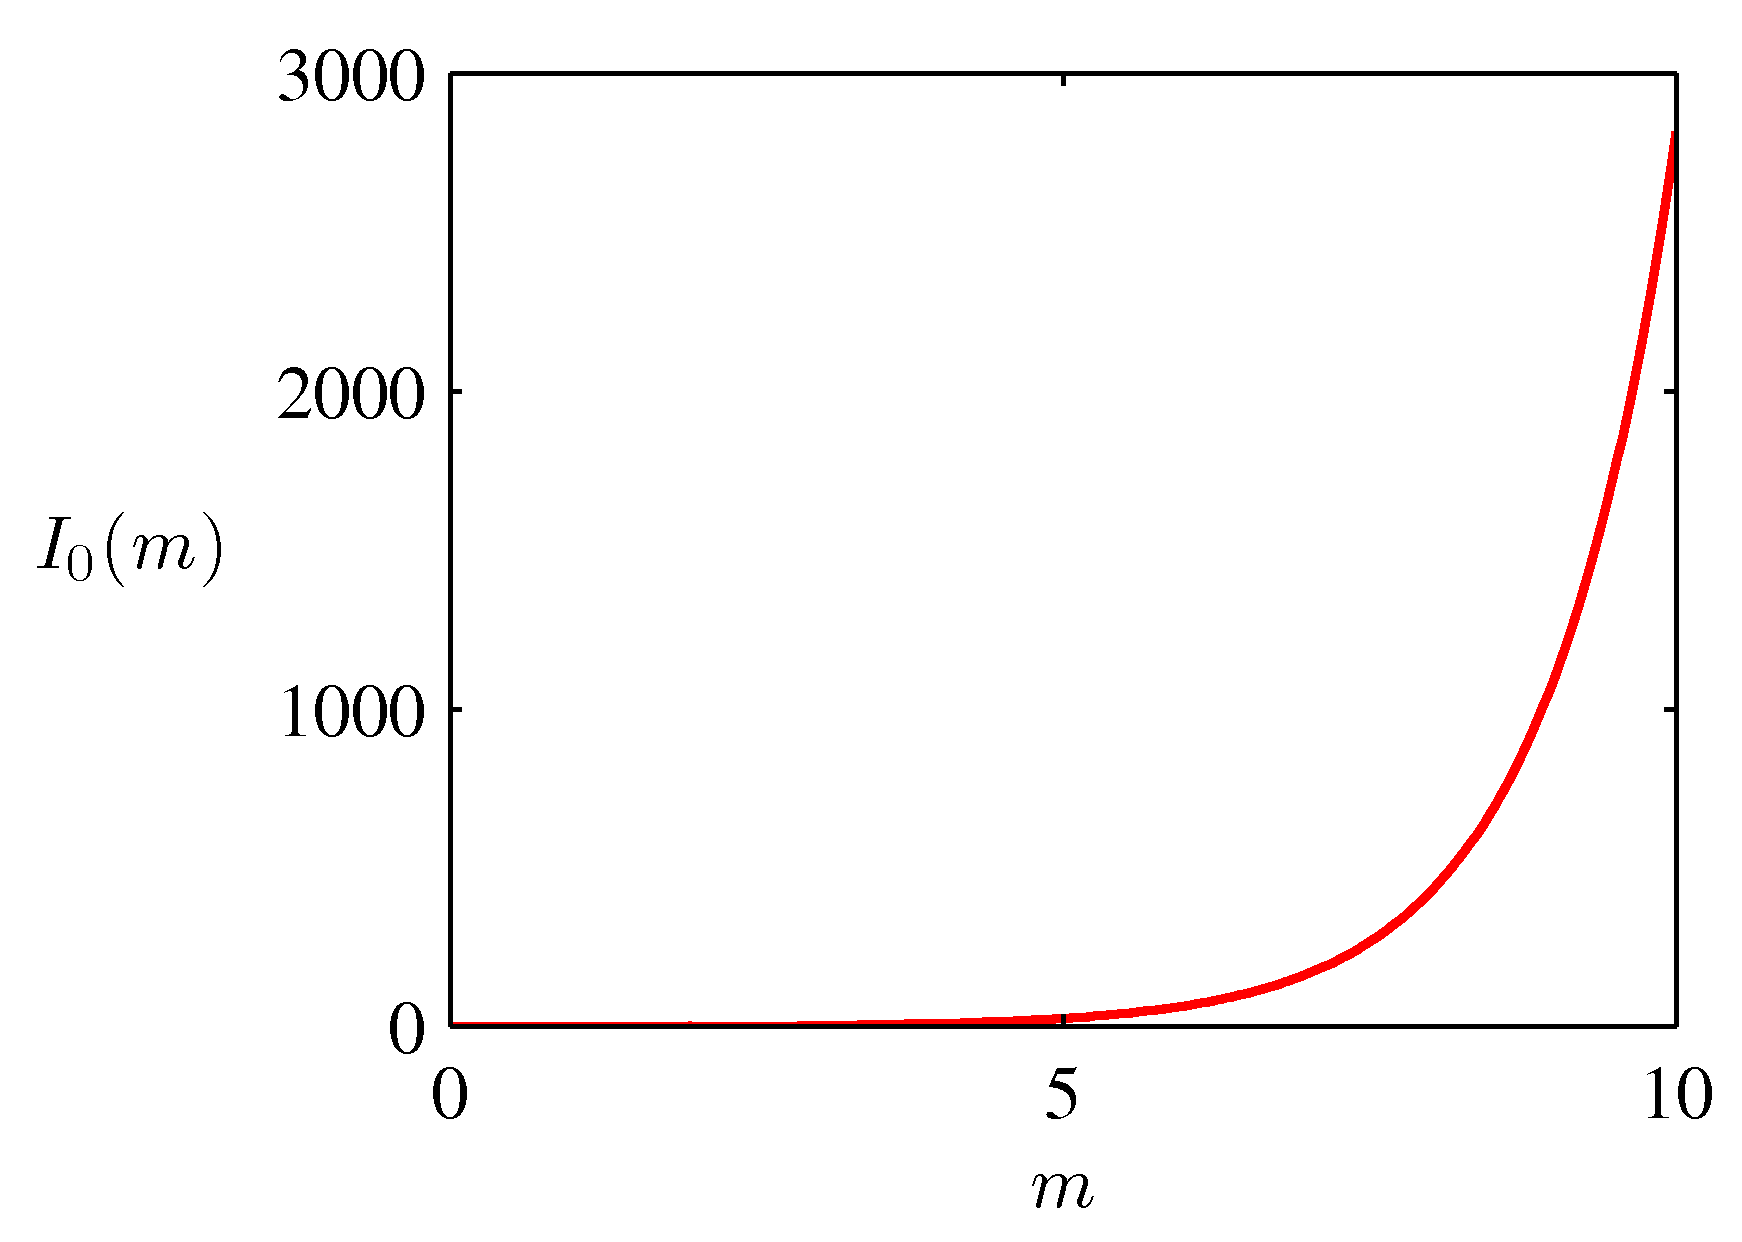
\includegraphics[scale=0.8]{Images/2-20a.png}
		\label{fig:2-20a}
		\end{minipage}
		\begin{minipage}[t]{0.5\linewidth}
		\centering
		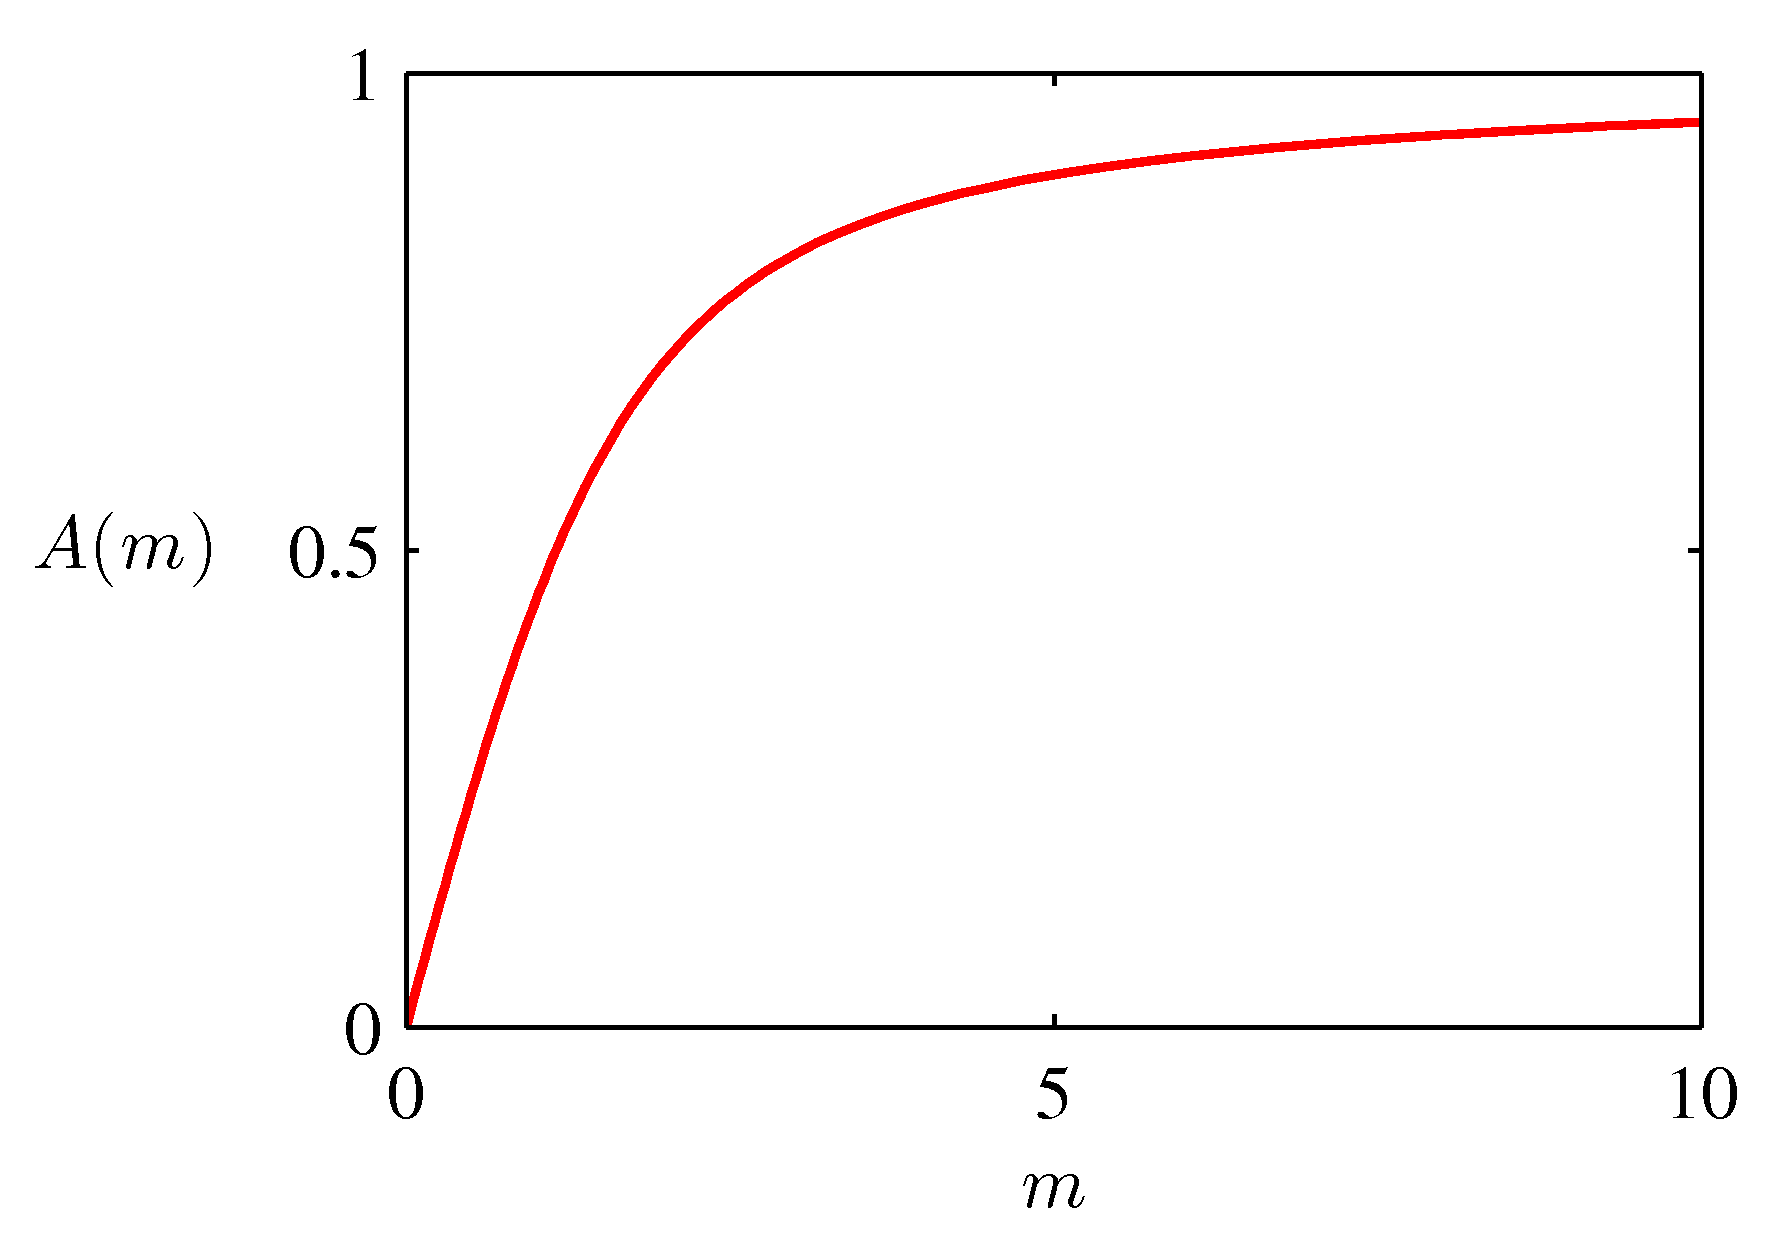
\includegraphics[scale=0.8]{Images/2-20b.png}
		\label{fig:2-20b}
		\end{minipage}
		\captionsetup{font={small}}
		\caption{(2.180)中的贝塞尔函数的图像,以及(2.186)中定义的函数$A(m)$的图像。}
	\end{figure}
	\noindent 于是可以得到\textcolor{red}{\textbf{——习题 2.53}}
	\begin{equation}
		\theta_0^{\mathrm{ML}}=\tan^{-1}\left\{\frac{\sum_n\sin\theta_n}{\sum_n\cos\theta_n}\right\}
	\end{equation}
	这其实就是(2.169)中二维笛卡尔空间中数据均值的结果。
	\indent 类似地,将(2.181)对于$m$求取最大值,并利用$I'_0(m)=I_1(m)$(Abramowitz and Stegun, 1965),可以得到
	\begin{equation}
		A(m_{\mathrm{ML}})=\frac{1}{N}\sum_{n=1}^N\cos (\theta_n-\theta_0^{\mathrm{ML}})
	\end{equation}
	其中代入了最大似然解$\theta_0^{\mathrm{ML}}$(回想一下,我们是在对$\theta$和$m$进行联合优化),并定义了
	\begin{equation}
		A(m)=\frac{I_1(m)}{I_0(m)}
	\end{equation}
	函数$A(m)$的图像如图2.20所示。利用三角恒等式(2.178),可以将(2.185)写成如下形式:
	\begin{equation}
		A(m_{\mathrm{ML}})=\left(\frac{1}{N}\sum_{n=1}^N\cos \theta_n\right)\cos \theta_0^{\mathrm{ML}} + \left(\frac{1}{N}\sum_{n=1}^N\sin \theta_n\right)\sin \theta_0^{\mathrm{ML}}
	\end{equation}
	(2.187)等号右侧的内容很容易处理,而且函数$A(m)$可以求数值逆。\\
	\indent 为了讨论的完整,在这里简单提及一些构造周期分布的其他方法。最简单的方法就是利用根据角度进行划分的直方图。这个方法十分简单灵活,但也有很大的局限性,我们将会在第2.5节中具体讨论直方图方法时详细讨论这个问题。另一种方法和von Mises分布,也是从欧几里得空间中的高斯分布开始的,但对单位圆采取的是边缘化而非条件化(Mardia and Jupp, 2000)。然而这样的处理会导致模型变得很复杂,在这里不做讨论。最后一种方法是通过将宽度为$2\pi$的连续区间映射到周期变量$(0,2\pi)$,这样的做法可以轻易将实轴上的任何分布(比如高斯分布)转化为周期分布,也就是用实轴把单位圆“包裹”起来。这样产生的分布也要比von Mises分布要复杂。\\
	\indent von Mises分布的一大局限性是其单峰性。通过将多个von Mises分布混合起来,我们可以得到一个用于多峰的周期变量建模的灵活框架。应用了von Mises分布的机器学习示例可以参考(Lawrence et al. , 2002),对于回归问题的条件密度建模,可以参考(Bishop and Nabney, 1996)。
	}
	\subsection{高斯混合模型}
	\textnormal{
	尽管高斯分布具有重要的分析性质,但在对实际的数据集进行建模的时候还是存在很大的局限性。比如图2.21所示的案例,这个数据集称为“Old Faithful”数据集,其中的数据是美国黄石国家公园的Old Faithful喷泉272次喷发的情况。\textcolor{red}{\textbf{——附录 A}}\ 每个数据的内容是喷发持续的时间(横轴)和到下次喷发的时间(纵轴),均以分钟为单位。可以看出,数据基本集中在两个区域中,一个单一的高斯分布明显不能贴切地表示这样的数据分布,但如果利用两个高斯分布的叠加,那么表征的效果会好很多。\\
	\indent 类似这样利用高斯分布等基础分布进行线性叠加形成新的概率模型的方法称为混合分布(mixture distributions, McLachlan and Basford, 1988; McLachlan and Peel, 2000)。从图2.22中可以看出高斯分布的线性组合可以形成非常复杂的概率密度。利用足够数量的高斯分布并调整其各自的均值、协方差和线性组合常数,几乎能够以任意精度逼近任何连续概率密度。
	\indent 于是我们可以写出$K$个高斯概率密度函数叠加的形式:
	\begin{equation}
		p(\bx)=\sum_{k=1}^K \pi_k\mathcal{N}(\bx|\bfMu_k, \bfSigma_k)
	\end{equation}
	\begin{figure}[H]
		\begin{minipage}[t]{0.5\linewidth}
		\centering
		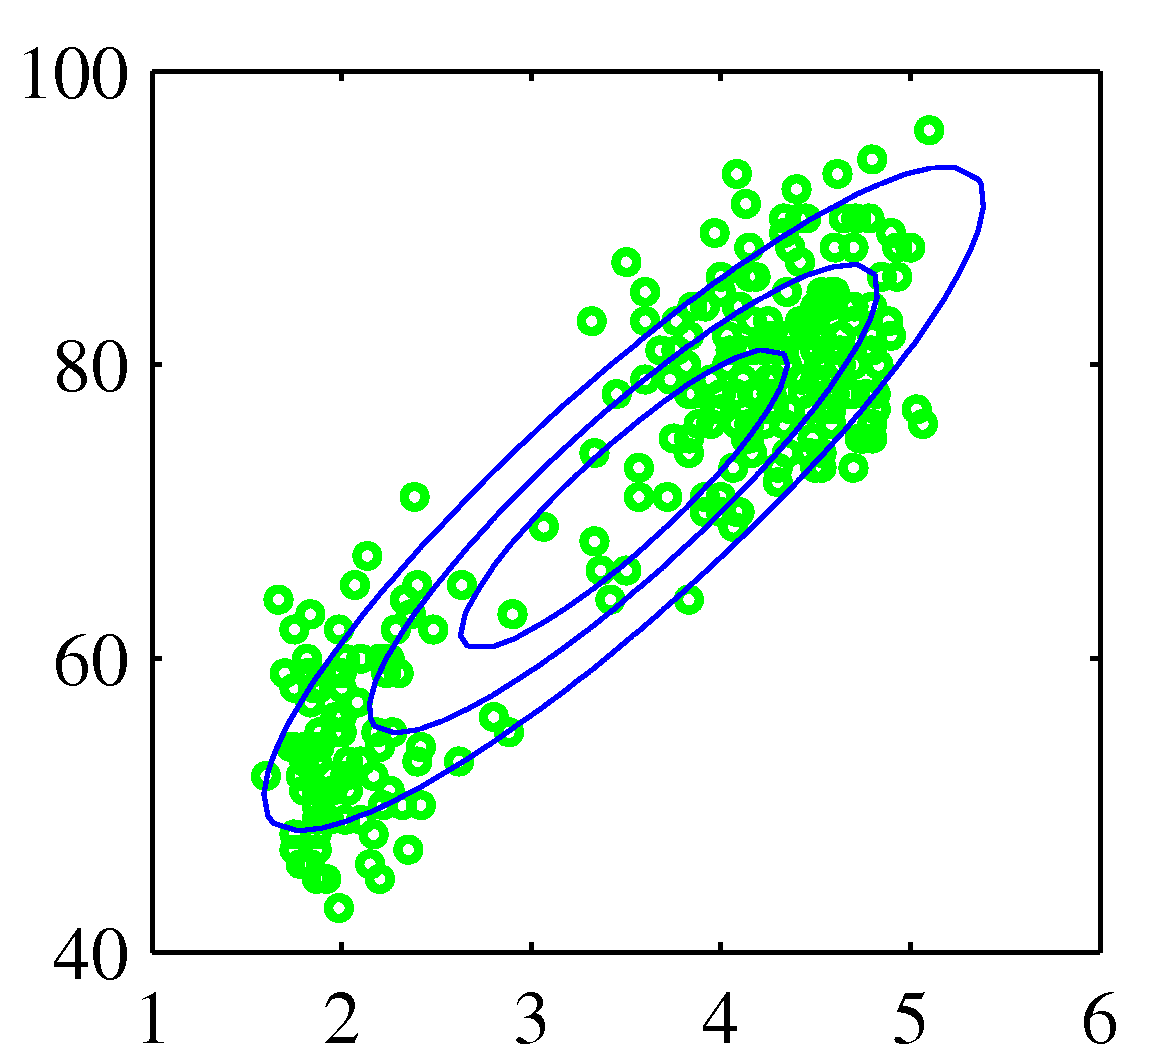
\includegraphics[scale=0.8]{Images/2-21a.png}
		\label{fig:2-21a}
		\end{minipage}
		\begin{minipage}[t]{0.5\linewidth}
		\centering
		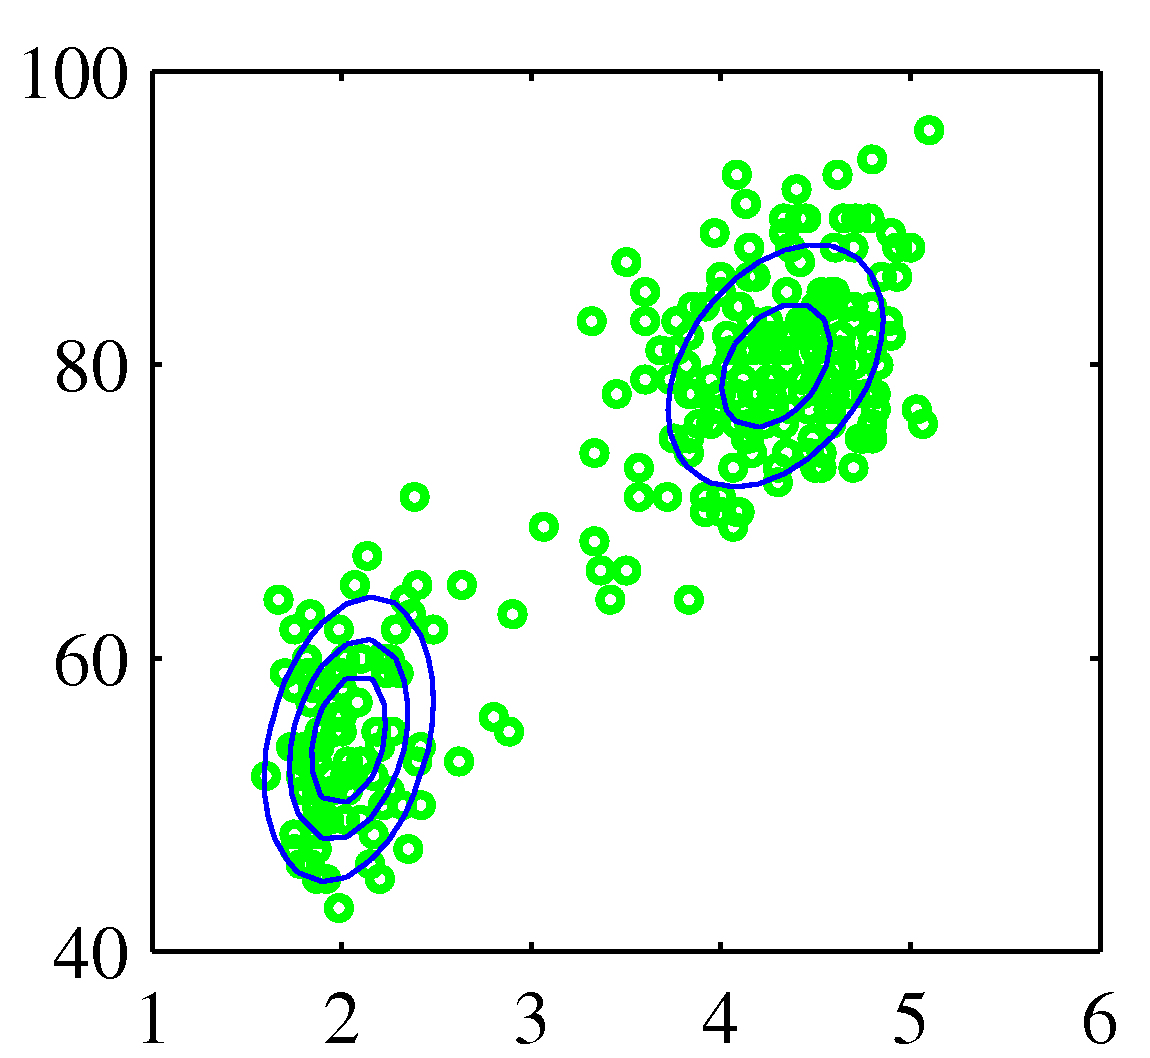
\includegraphics[scale=0.8]{Images/2-21b.png}
		\label{fig:2-21b}
		\end{minipage}
		\captionsetup{font={small}}
		\caption{“Old Faithful”数据集,蓝色曲线表示概率密度。左图是利用最大似然得到的单一的高斯分布。很明显,单一的高斯分布很难描述数据划分成两个明显区域这一特点,而是处于数据的中心,数据相当稀疏的位置。右图中利用最大似然得到两个叠加的高斯分布,效果就好得多了。具体的手段将在第9章中详细介绍。}
		\centering
		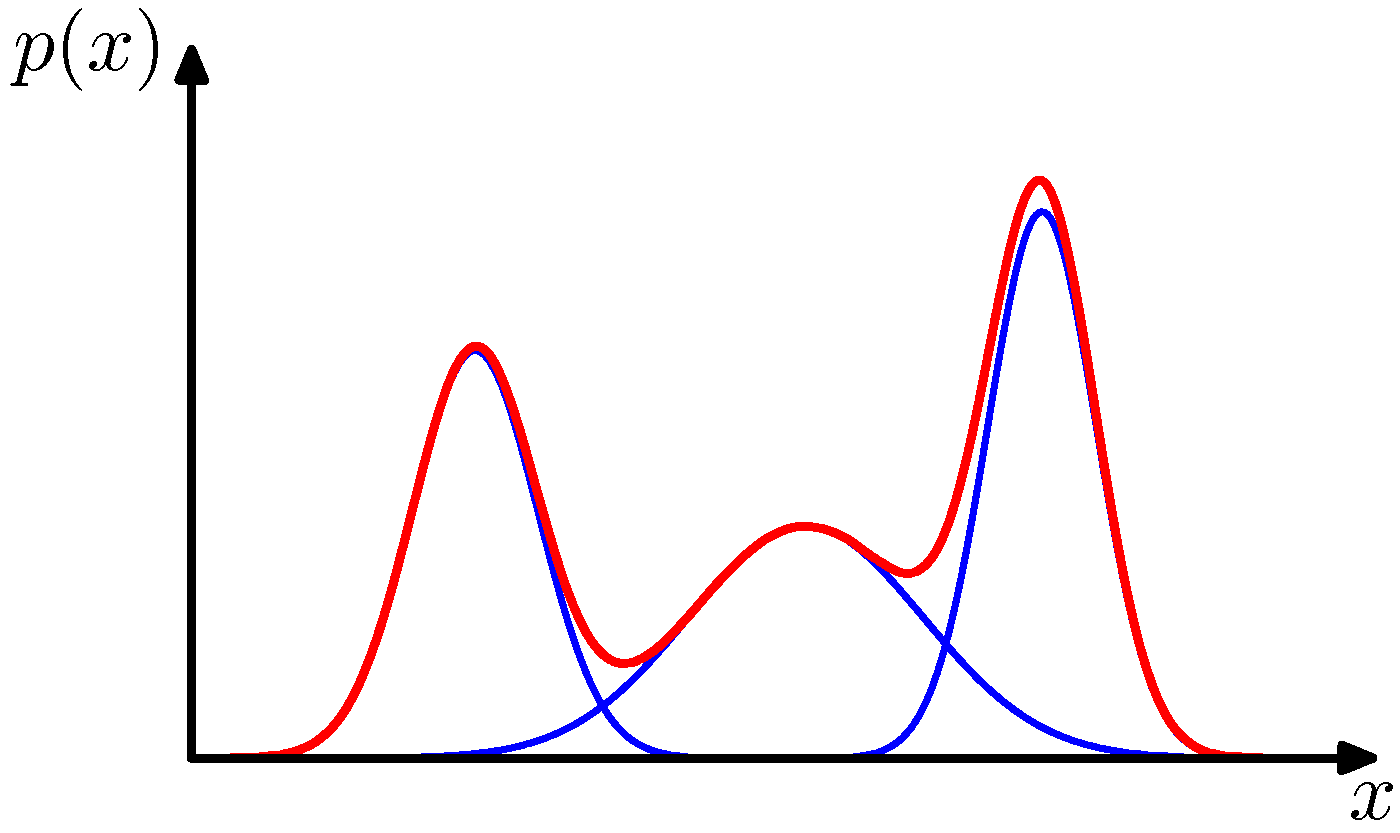
\includegraphics[scale=0.8]{Images/2-22.png}
		\captionsetup{font={small}}
		\caption{一维情况下的高斯混合分布,蓝色曲线为3个高斯分布(在线性组合中各自带有系数),红色曲线为其混合分布。}
		\label{fig:2-22}
		\begin{minipage}[t]{0.3\linewidth}
		\centering
		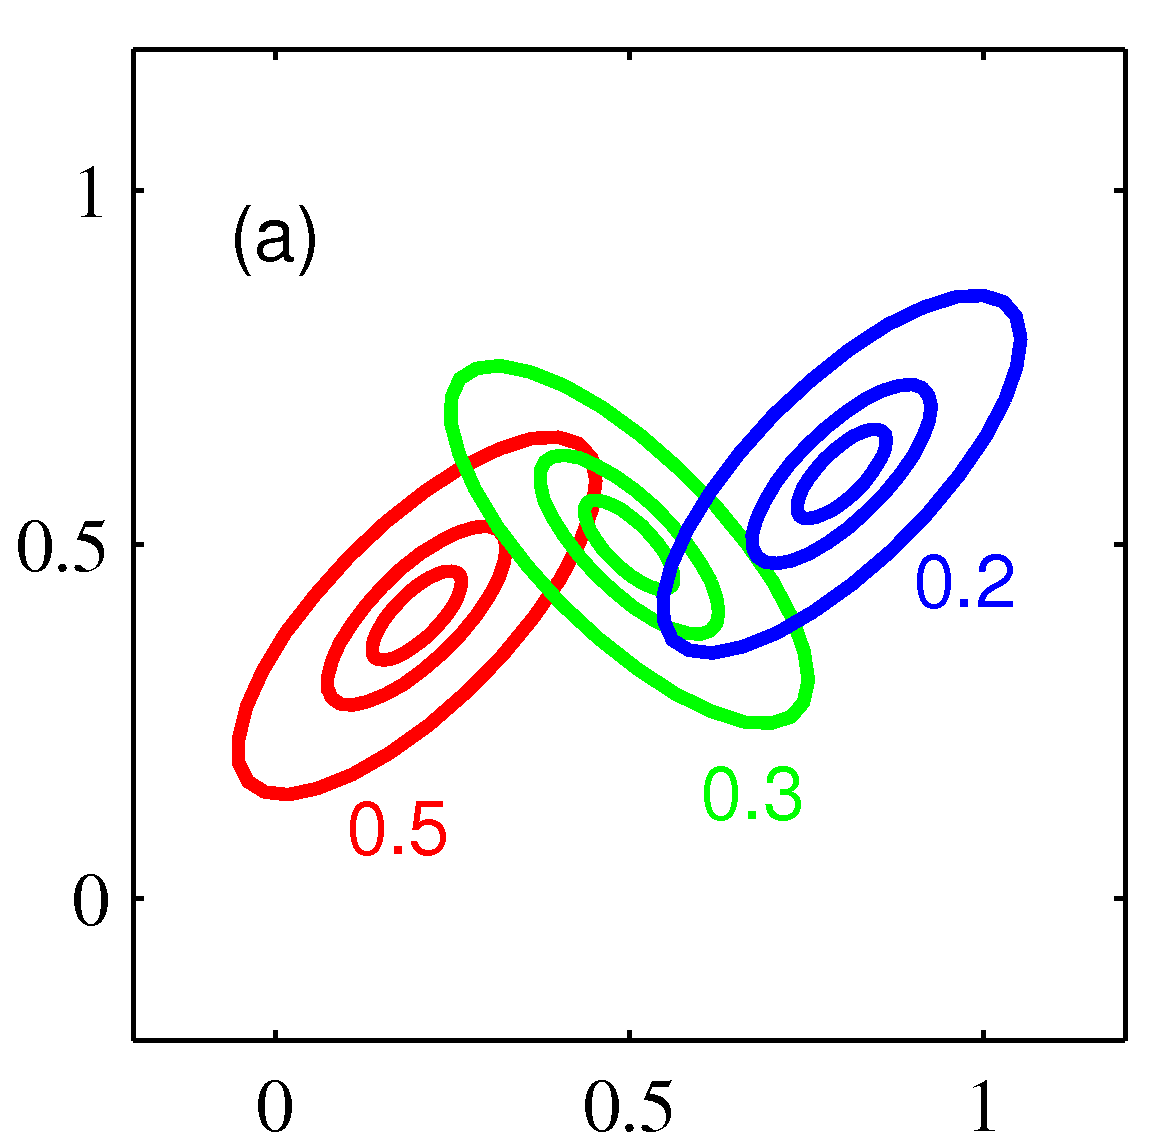
\includegraphics[scale=0.8]{Images/2-23a.png}
		\label{fig:2-23a}
		\end{minipage}
		\begin{minipage}[t]{0.3\linewidth}
		\centering
		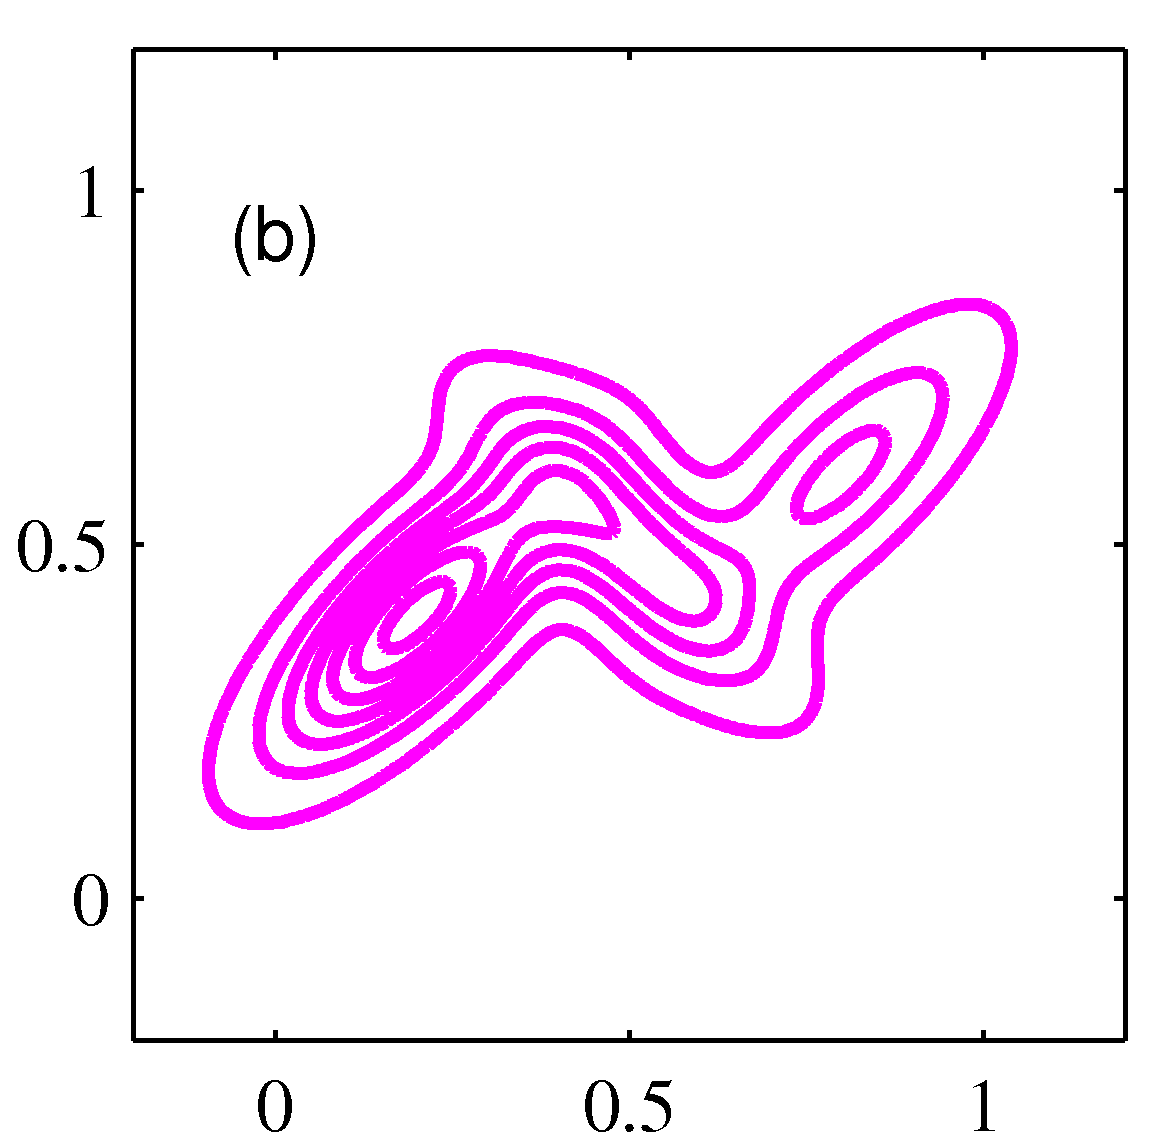
\includegraphics[scale=0.8]{Images/2-23b.png}
		\label{fig:2-23b}
		\end{minipage}
		\begin{minipage}[t]{0.3\linewidth}
		\centering
		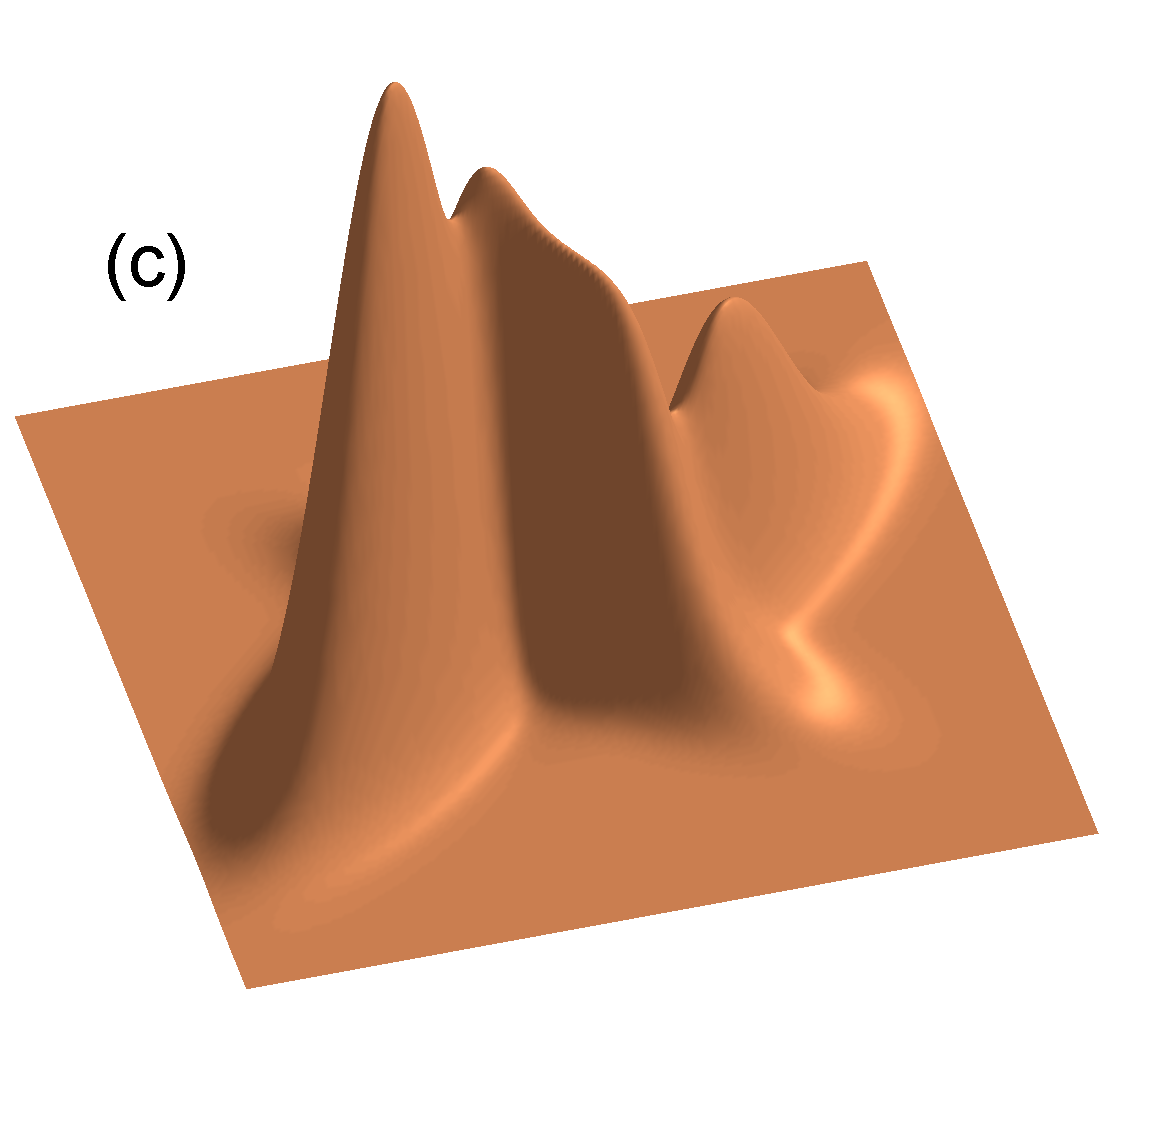
\includegraphics[scale=0.8]{Images/2-23c.png}
		\label{fig:2-23c}
		\end{minipage}
		\captionsetup{font={small}}
		\caption{二维空间中3个高斯分布的混合模型。(a)为每个混合组件各自的等高线图,分别表示为红色、蓝色和绿色,并标出了各自的混合系数;(b)为混合分布的边缘概率密度$p(\bx)$;(c)为分布$p(\bx)$的空间图像。}
	\end{figure}
	这就是高斯混合模型(mixture of Gaussians)。每个高斯概率密度$\mathcal{N}(\bx|\bfMu_k, \bfSigma_k)$都是混合模型中的组件(component),各自都有自己的均值$\bfMu_k$和协方差$\bfSigma_k$。包含3个组件的高斯混合模型示例如图2.23所示。
	\indent 在本节中我们利用高斯分布作为组件来介绍混合模型的框架。一般情况下,混合模型可以包含其他分布的线性组合。例如,在第9.3.3节中我们会介绍离散变量的伯努利分布的混合模型。\\
	\indent (2.188)中的参数$\pi_k$称为混合系数(mixing coefficients)。如果我们将(2.188)的两侧同时对$\bx$积分,并留意到$p(\bx)$和每个高斯分布组件都是归一化的,可以得到
	\begin{equation}
		\sum_{k=1}^K \pi_k = 1
	\end{equation}
	同时,在$\mathcal{N}(\bx|\bfMu_k, \bfSigma_k) \geqslant 0$的条件下,使得$p(\bx)\geqslant 0$的充分条件是对于任意的$k$,$\pi_k \geqslant 0$。与(2.189)联合在一起,得到条件
	\begin{equation}
		0 \leqslant \pi_k \leqslant 1
	\end{equation}
	于是可以看出,混合系数是满足概率所要求的条件的。\\
	\indent 根据加法和乘法规则,边缘概率密度为
	\begin{equation}
		p(\bx) = \sum_{k=1}^K p(k)p(\bx|k)
	\end{equation}
	这个等式等价于(2.188),可以将$\pi_k=p(k)$看成是融合第$k$个组件时的先验概率,概率密度$\mathcal{N}(\bx|\bfMu_k, \bfSigma_k)=p(\bx|k)$可以看成是给定$k$的条件下$\bx$的概率。我们会在接下来的章节中看到,后验分布$p(k|\bx)$将会扮演重要的角色,它也被称为responsibilities。根据贝叶斯定理,
	\begin{equation}
	\begin{split}
		\gamma_k(\bx) &\equiv p(k|\bx) \\
		&= \frac{p(k)p(\bx|k)}{\sum_lp(l)p(\bx|l)} \\
		&= \frac{\pi_k\mathcal{N}(\bx|\bfMu_k,\bfSigma_k)}{\sum_l \pi_l \mathcal{N}(\bx|\bfMu_l, \bfSigma_l)}
	\end{split}
	\end{equation}
	我们会在第9章中利用概率更加详细地讨论混合分布。\\
	\indent 高斯混合分布由参数$\boldsymbol{\pi}, \bfMu$和$\bfSigma$控制,其中$\boldsymbol{\pi} \equiv \{\pi_1,...,\pi_K\}, \bfMu \equiv \{\bfMu_1,...,\bfMu_K\}, \bfSigma \equiv \{\bfSigma_1,...,\bfSigma_K\}$。设定这些参数的方法之一就是利用最大似然。根据(2.188),似然函数为
	\begin{equation}
		\ln p(\mathbf{X}|\boldsymbol{\pi},\bfMu,\bfSigma)=\sum_{n=1}^N \ln \left\{\sum_{k=1}^K \pi_k \mathcal{N}(\bx_n|\bfMu_k, \bfSigma_k)\right\}
	\end{equation}
	其中$\mathbf{X}=\{\bx_1,...,\bx_N\}$。这很明显要比单一高斯分布的情况要复杂很多,因为在对数内包含了关于$k$的求和。因此,参数的最大似然求解不再是具有闭式解析解的了。似然函数最大化的方法之一是利用迭代数值优化 (Fletcher, 1987; Nocedal and Wright, 1999; Bishop and Nabney, 2008),或者利用期望最大化(EM, expectation maximization)这一框架,这一方法将在第9章中详细讨论。
	}
	\section{指数型分布族}
	\insertline\\
	\textnormal{
	\indent 在本章节此前的内容中,我们所看到的概率分布(除了高斯混合模型)都是一个广大的分布类别中的特例,这个分布类别叫做指数型分布族(exponential family, Duda and Hart, 1973; Bernardo and Smith, 1994)。指数型分布族中的成员有很多共同的重要性质,对于一般情况进行讨论会比较具有启发的意义。\\
	\indent 给定参数$\bfeta$的情况下$\bx$的指数型分布族可以由以下形式的分类集合定义:
	\begin{equation}
		p(\bx|\bfeta)=h(\bx)g(\bfeta)\exp\{\bfeta^{\rmT}\mathbf{u}(\bx)\}
	\end{equation}
	其中$\bx$可以是标量也可以是向量,可以是离散变量也可以是连续变量;$\bfeta$称为分布的自然参数(natural parameters),$\mathbf{u}(\bx)$为$\bx$的函数。函数$g(\bfeta)$可以看成是分布的归一化系数,于是一定满足
	\begin{equation}
		g(\bfeta)\int h(\bx)\exp \{\bfeta^{\rmT}\mathbf{u}(\bx)\}\ \mathrm{d}\bx = 1
	\end{equation}
	其中,如果$\bx$为离散变量,就把积分替换成求和。\\
	\indent 我们从这个章节比较靠前的内容中介绍的分布开始,证明这些分布确实是属于指数型分布族的。首先,对于伯努利分布
	\begin{equation}
		p(x|\mu)=\mathrm{Bern}(x|\mu)=\mu^x(1-\mu)^{1-x}
	\end{equation}
	将等号右侧的内容写成对数的指数形式,可得
	\begin{equation}
	\begin{split}
		p(x|\mu) &= \exp\{x\ln \mu + (1-x)\ln (1-\mu)\}\\
		&= (1-\mu) \exp\left\{\ln \left(\frac{\mu}{1-\mu}x\right)\right\}
	\end{split}
	\end{equation}
	与(2.194)做一下对比,马上可以看出
	\begin{equation}
		\eta=\ln (\frac{\mu}{1-\mu})
	\end{equation}
	根据这个方程可以直接写成$\eta=\sigma(\eta)$的形式,也就是
	\begin{equation}
		\sigma(\eta)=\frac{1}{1+\exp(-\eta)}
	\end{equation}
	这个函数称为logistic sigmoid函数。于是我们就可以将伯努利分布写成(2.194)的形式:
	\begin{equation}
		p(x|\eta)=\sigma(-\eta)\exp(\eta x)
	\end{equation}
	其中我们使用了性质$1-\sigma(\eta)=\sigma(-\eta)$,根据(2.199)可以很容易地证明这一点。与(2.194)对比一下,可以看出
	\begin{align}
		u(x) &= x \\
		h(x) &= 1 \\
		g(\eta) &= \sigma(-\eta)
	\end{align}
	\indent 接下来我们研究一下多项分布。对于单一的$\bx$,多项分布的形式为
	\begin{equation}
		p(\bx|\bfMu)=\prod_{k=1}^M \mu_k^{x_k}=\exp\left\{\sum_{k=1}^M x_k \ln \mu_k\right\}
	\end{equation}
	其中$\bx=\{x_1,...,x_M\}^{\rmT}$。和上一个分布一样,可以将它写成(2.194)这样的标准形式
	\begin{equation}
		p(\bx|\bfeta) = \exp\{\bfeta^{\rmT}\bx\}
	\end{equation}
	其中$\eta_k=\ln \mu_k$,并定义了$\bfeta=(\eta_1,...,\eta_M)^{\rmT}$。与(2.194)对比一下,可以得到
	\begin{align}
		\mathbf{u}(\bx) &= \bx \\
		h(\bx) &= 1 \\
		g(\bfeta) &= 1
	\end{align}
	需要注意到参数$\eta_k$之间并非是相互独立的,因为它们必须满足条件
	\begin{equation}
		\sum_{k=1}^M  \mu_k = 1
	\end{equation}
	于是,如果给定了所有参数$\mu_k$中$M-1$个参数的值,那么剩下的一个参数值就是确定的了。在某些情况下,将最后一个参数删除,仅保留$M-1$个参数,会让问题更加简单一些。利用(2.209)就可以项$\mu_M$删除,$\{\mu_M\}$中也仅剩下$k=1,...,M-1$这$M-1$个参数。需要注意的是,剩下的这些参数仍然满足如下的限制:
	\begin{equation}
		0 \leqslant \mu_k \leqslant 1, \  \sum_{k=1}^{M-1}\mu_k \leqslant 1
	\end{equation}
	利用约束(2.209),多项分布的表达形式可以写成
	\begin{equation}
	\begin{split}
		&\exp\left\{\sum_{k=1}^M x_k \ln \mu_k\right\} \\
		= &\exp\left\{\sum_{k=1}^{M-1}x_k \ln \mu_k + \left(1-\sum_{k=1}^{M-1}x_k\right) \ln \left(1-\sum_{k=1}^{M-1}\mu_k\right)\right\} \\
		= &\exp\left\{\sum_{k=1}^{M-1}x_k \ln \left(\frac{\mu_k}{1-\sum_{j=1}^{M-1}\mu_j}\right) + \ln \left(1-\sum_{k=1}^{M-1}\mu_k\right)\right\}
	\end{split}
	\end{equation}
	令
	\begin{equation}
		\ln \left(\frac{\mu_k}{1-\sum_j \mu_j}\right) = \eta_k
	\end{equation}
	可以通过将等式两侧的内容全部关于$k$求和,然后经过一些变换来解出$\mu_k$,
	\begin{equation}
		\mu_k = \frac{\exp(\eta_k)}{1+\sum_j \mu_j}
	\end{equation}
	这个函数称为softmax函数,或者称为归一化指数(normalized exponential)。利用这个表示多项分布,可以写成
	\begin{equation}
		p(\bx|\bfeta)=\left(1+\sum_{k=1}^{M-1}\exp(\eta_k)\right)^{-1} \exp(\bfeta^{\rmT}\bx)
	\end{equation}
	这就是多峰分布写成指数型分布族标准形式的结果,参数$\bfeta=\{\eta_1,...,\eta_{M-1},0\}^{\rmT}$,且
	\begin{align}
		\mathbf{u}(\bx)&=\bx \\
		h(\bx)&= 1 \\
		g(\bfeta) &= \left(1+\sum_{k=1}^{M-1}\exp(\eta_k)\right)^{-1}
	\end{align}
	\indent 最后我们来研究一下高斯分布。对于一元高斯分布,
	\begin{align}
		p(x|\mu,\sigma^2) &= \frac{1}{(2\pi \sigma^2)^{1/2}}\exp\left\{-\frac{1}{2\sigma^2}(x-\mu)^2\right\} \\
		&= \frac{1}{(2\pi\sigma^2)^{1/2}}\exp\left\{-\frac{1}{2\sigma^2}x^2+\frac{\mu}{\sigma^2}x - \frac{1}{2\sigma^2}\mu^2\right\}
	\end{align}
	经过一些简单的变形,可以得到其标准的形式\textcolor{red}{\textbf{——习题 2.57}}
	\begin{align}
		\bfeta &= \left(\begin{matrix} \mu/\sigma^2 \\ -1/2\sigma^2 \end{matrix}\right) \\
		\mathbf{u}(x) &= \left(\begin{matrix} x \\ x^2 \end{matrix}\right)\\
		h(x) &= (2\pi)^{-1/2}\\
		g(\bfeta) &= (-2\eta_2)^{1/2} \exp \left(\frac{\eta_1^2}{4\eta_2}\right)
	\end{align}
	}
	\subsection{最大似然与充分统计量}
	\textnormal{
	首先来利用最大似然方法估计指数型分布族(2.194)中的参数向量$\bfeta$。对(2.195)等式两边同时关于$\bfeta$求梯度,
	\begin{equation}
		\nabla g(\bfeta) \int h(\bx)\exp\{\bfeta^{\rmT}\mathbf{u}(\bx)\}\ \mathrm{d}\bx + g(\bfeta)\int h(\bx)\exp\{\bfeta^{\rmT}\mathbf{u}(\bx)\}\mathbf{u}(\bx)\ \mathrm{d}\bx =0
	\end{equation}
	将它整理一下,再次利用(2.195),可得
	\begin{equation}
		-\frac{1}{g(\bfeta)}\nabla g(\bfeta) = g(\bfeta)\int h(\bx)\exp\{\bfeta^{\rmT}\mathbf{u}(\bx)\} \mathbf{u}(\bx) \ \mathrm{d}\bx = \mathbb{E}[\mathbf{u}(\bx)]
	\end{equation}
	于是可以得到
	\begin{equation}
		-\nabla \ln g(\bfeta) = \mathbb{E}[\mathbf{u}(\bx)]
	\end{equation}
	需要注意的是,$\mathbf{u}(\bx)$的协方差可以用$g(\bfeta)$的二阶导数表示,而且更高阶的矩同样可以。\textcolor{red}{\textbf{——习题 2.58}}\ 所以只要我们能够将属于指数型分布族的分布进行归一化,就可以通过求导来求取其各阶的矩。\\
	\indent 现在假设有一组独立同分布的数据$\mathbf{X}=\{\bx_1,...,\bx_N\}$,似然函数为
	\begin{equation}
		p(\mathbf{X}|\bfeta)=\left(\prod_{n=1}^N h(\bx_n)\right)g(\bfeta)^N \exp \left\{\bfeta^{\rmT}\sum_{n=1}^N \mathbf{u}(\bx_n)\right\}
	\end{equation}
	令$\ln p(\mathbf{X|\bfeta})$关于$\bfeta$的导数等于0,可以得到最大似然估计$\bfeta_{\mathrm{ML}}$应当满足的条件
	\begin{equation}
		-\nabla \ln g(\bfeta_{\mathrm{ML}})=\frac{1}{N}\sum_{n=1}^N\mathbf{u}(\bx_n)
	\end{equation}
	理论上来说可以利用它来确定$\bfeta_{\mathrm{ML}}$。可以看出,最大似然解与数据有关的部分仅仅是$\sum_n\mathbf{u}(x)$而已,所以它被称为分布(2.194)的充分估计量。我们并不需要将整个数据集都保存下来,只需要将充分估计量的值存下来就可以了。举个例子,对于伯努利分布,$\mathbf{u}(\bx)$的内容仅仅是一个$x$而已,所以只需要留下$\{x_n\}$的总和就足够了;对于高斯分布就要复杂一些,它的$\mathbf{u}(\bx)=(x,x^2)^{\rmT}$,所以要计算$\{x_n\}$的总和,以及$\{x_n^2\}$的总和。\\
	\indent 如果取极限$N \rightarrow \infty$,那么(2.228)等号右侧的内容就变成了$\mathbb{E}[\mathbf{u}(\bx)]$,与(2.226)做一下对比,可以看出在这个极限下,$\bfeta_{\mathrm{ML}}$将与$\bfeta$的真实值相等。\\
	\indent 实际上,这个充分条件同样适用于贝叶斯推断,不过我们要在第8章中,连同图模型这一强大工具进行更加深刻的研究。
	}
	\subsection{共轭先验}
	\textnormal{
	我们已经很多次遇到共轭先验这个概念了,在伯努利分布(其共轭先验为beta分布)和高斯分布(高斯分布均值的先验分布为高斯分布,精度的先验分布为维希特分布)的讨论中都有提及。一般而言,对于给定的概率分布$p(\bx|\bfeta)$,我们都可以找到一个与似然函数共轭的先验$p(\bfeta)$,使得后验分布与先验分布具有相同的函数形式。对于任何属于指数型分布族的分布(2.194),都存在如下形式的先验分布
	\begin{equation}
		p(\bfeta|\boldsymbol{\chi},\nu)=f(\boldsymbol{\chi},\nu)g(\bfeta)^{\nu}\exp\{\nu \bfeta^{\rmT}\boldsymbol{\chi}\}
	\end{equation}
	其中$f(\boldsymbol{\chi},\nu)$为归一化系数,$g(\bfeta)$就是(2.194)中的$g(\bfeta)$。为了证明它与似然函数确实是共轭的,我们将先验(2.229)乘以似然函数(2.227),从而得到后延分布,不考虑归一化常数,结果为
	\begin{equation}
		p(\bfeta|\mathbf{X},\boldsymbol{\chi},\nu) \propto g(\bfeta)^{\nu+N}\exp\left\{\bfeta^{\rmT}\left(\sum_{n=1}^N\mathbf{u}(\bx_n)+\nu \boldsymbol{\chi}\right)\right\}
	\end{equation}
	很明显它与(2.229)的形式是一样的,于是确定了这个先验是共轭先验。此外,参数$\nu$可以看成是先验分布中假想数据里有效数据的数量,在给定$\boldsymbol{\chi}$的条件下,每个有效数据都对充分统计量$\mathbf{u}(\bx)$存在影响。
	}
	\subsection{无信息先验}
	\textnormal{
	在一些概率推断的应用中,我们可能会有先验知识,而且可以用先验分布表示它。举例而言,如果将某些变量的概率先验值设为0,那么后延分布也必然会将该变量设为0,不管后续的数据都是什么样的。但在大多数情况下,我们可能完全不知道分布是什么样的形式。这样的情况下,我们会求取另一种形式的先验,也就是无信息先验(noninformative prior),无信息先验的目的就是使先验信息对后验分布的影响尽可能地小(Jeffreys, 1946; Box and Tiao, 1973; Bernardo and Smith, 1994)。这样的做法有时称为“让数据为自己说话”。\\
	\indent 对于一个由参数$\lambda$控制的分布$p(x|\lambda)$,我们可能会理所应当地认为$p(\lambda)=\mathrm{const}$这样的先验分布是比较合适的。如果$\lambda$是一个具有$K$个可能取值的离散变量,那么按照这种方法,将每种取值的先验概率设定为$1/K$似乎是比较合适的。然而,对于连续变量而言,这种方法有两个非常糟糕的缺陷。首先,如果参数$\lambda$没有确定的界限,那么这个先验分布就可能不满足归一化条件,因为关于$\lambda$的积分可能是发散的。这样的先验称为反常(improper)先验。在实际的应用中,如果对应的后验是正常(proper)的,那么往往意味着这个反常先验可以被归一化,那么就是可以使用的。举个例子,如果对高斯分布的均值赋予一个均匀分布作为先验分布,那么我们一旦进行至少一个数据点的概率更新,均值的后验分布就会是正常的。\\
	\indent 这个方法的第二个困难之处在于变量发生非线性变换(1.27)时概率密度的变换方式。假设函数$h(\lambda)$为常数,并做了变换$\lambda = \eta^2$,那么$\hat(h)(\eta)=h(\eta^2)$也是常数。然而,如果我们将概率密度$p_{\lambda}(\lambda)$设定为常数,那么根据(1.27),$\eta$的概率密度为
	\begin{equation}
		p_{\eta}(\eta)=p_{\lambda}(\lambda)\left|\frac{\mathrm{d}{\lambda}}{\mathrm{d}{\eta}}\right| = p_{\lambda}(\eta^2)2\eta \propto \eta
	\end{equation}
	那么$\eta$的分布就不再是常数了。在最大似然方法中不会出现这个问题,因为似然函数$p(x|\lambda)$只是一个关于$\lambda$的函数而已,所以可以自由使用任何操作参数的方法。然而,如果想要选取常数作为先验分布,那么就必须选取合适的参数表达形式。\\
	\indent 现在我们研究两个简单的无信息先验的案例(Berger, 1985)。首先,如果概率密度的形式为
	\begin{equation}
		p(x|\mu)=f(x-\mu)
	\end{equation}
	这里的参数$\mu$称为位置参数(location parameter)。这样的一类概率密度满足变换不变性(translation invariance),因为如果令$\hat{x}=x+c$,那么
	\begin{equation}
		p(\hat{x}|\hat{\mu})=f(\hat{x}-\hat{\mu})
	\end{equation}
	其中$\hat{mu}=\mu+c$。所以新变量的概率密度与原始的概率密度具有相同的形式。我们当然很愿意选择满足这样条件的先验分布,这样的先验分布可以使$A \leqslant \mu \leqslant B$区间内的概率质量完整平移到区间$A-c \leqslant \mu \leqslant B-c$,也就是
	\begin{equation}
		\int_A^B p(\mu)\ \mathrm{d}\mu = \int _{A-c}^{B-c}p(\mu)\ \mathrm{d}\mu = \int_A^B p(\mu-c)\ \mathrm{d}\mu
	\end{equation}
	由于这个等式对于任意的$A$和$B$均成立,则
	\begin{equation}
		p(\mu-c)=p(\mu)
	\end{equation}
	也就是说$p(\mu)$是常数。位置参数的一个最典型的例子就是高斯分布的均值$\mu$。我们已经看到,这种情况下$\mu$的共轭先验分布是一个高斯分布$p(\mu|\mu_0,\sigma_0^2)=\calN(\mu|\mu_0,\sigma_0^2)$,而且如果取极限$\sigma_0^2 \rightarrow \infty$,就可以得到无信息先验了。根据(2.141)和(2.142),可以看出在这个情况下,先验分布将不再对$\mu$的后验分布造成任何影响。\\
	\indent 接下来讨论第二个例子。假设概率密度的形式为
	\begin{equation}
		p(x|\sigma)=\frac{1}{\sigma}f\left(\frac{x}{\sigma}\right)
	\end{equation}
	其中$\sigma>0$。需要注意的是,如果$f(x)$是归一化的,那么这个概率密度也是可以归一化的。\textcolor{red}{\textbf{——习题 2.59}}\ 这里的参数$\sigma$称为缩放参数(scale parameter),而且这一概率密度满足缩放不变性(scale parameter),因为如果令$\hat{x}=cx$,那么
	\begin{equation}
		p(\hat{x}|\hat{\sigma})=\frac{1}{\hat{\sigma}}f\left(\frac{\hat{x}}{\hat{\sigma}}\right)
	\end{equation}
	其中$\hat{\sigma}=c\sigma$。这个变换是尺度上的缩放,就像把米换算成千米一样,我们也很愿意选择满足这样条件的分布作为先验分布。对于某个区间$A \leqslant \sigma \leqslant B$和它对应的缩放区间$A/c \leqslant \sigma \leqslant B/c$,先验分布在这两个区间内的概率质量应该是相等的,即
	\begin{equation}
		\int_A^B p(\sigma)\ \mathrm{d}\sigma =\int_{A/c}^{B/c} p(\sigma)\ \mathrm{d}\sigma = \int_A^B p\left(\frac{1}{c}\sigma\right)\frac{1}{c}\ \mathrm{d}\sigma
	\end{equation}
	而且这个关系对于任意的$A$和$B$恒成立,于是有
	\begin{equation}
		p(\sigma)=p\left(\frac{1}{c}\sigma\right)\frac{1}{c}
	\end{equation}
	于是$p(\sigma) \propto 1/\sigma$。需要再次注意的是,这是一个反常先验,因为区间$0 \leqslant \sigma \leqslant \infty$上的积分是发散的。对于一个缩放参数,有时候使用参数的对数形式研究问题也是比较方便的。根据变换公式(1.27),可以看出$p(\ln \sigma)$是常数。所以先验在区间$1 \leqslant \sigma \leqslant 10$内的概率质量与区间$10 \leqslant \sigma \leqslant 100$和$100 \leqslant \sigma \leqslant 1000$内是相同的。\\
	\indent 缩放参数的一个典型案例就是高斯分布的标准差$\sigma$,当然是在确定了位置参数$\mu$之后。因为
	\begin{equation}
		\calN(x|\mu,\sigma^2) \propto \sigma^{-1} \exp\{-(\widetilde{x}/\sigma)^2\}
	\end{equation}
	其中$\widetilde{x}=x-\mu$。正如早些时候讨论过的,利用精度$\lambda = 1/\sigma^2$来开展下一步会比利用$\sigma$本身要方便很多。根据概率密度的变换规则,可以看出一个满足条件$p(\sigma) \propto 1/\sigma$的分布对应于$\lambda$的分布$p(\lambda)\propto 1/\lambda$。根据(2.146),可以看出$\lambda$的共轭先验为Gamma分布$\mathrm{Gam}(\lambda|a_0,b_0)$。\textcolor{red}{\textbf{——第2.3节}}\ 如果$a_0=b_0=0$,那么它就是一个无信息先验。如果对于$\lambda$的后验分布计算(2.150)和(2.151)的结果,可以得到在$a_0=b_0=0$的情况下,后验分布将仅与数据相关,而与先验无关。
	}
	\section{非参数方法}
	\insertline
	\textnormal{
	\indent 在本章中,我们一直专注于某些特定形式的概率分布,这些概率分布都由数量较少的参数控制,而这些参数是根据数据集来确定的。这样的方法称为概率密度建模的参数方法(parametric approach)。这样的方法存在很明显的局限性,那就是我们选定的分布形式不一定能够很好地描述数据的模式,于是它的预测能力也是比较差的。举例而言,如果数据的来源是一个多项分布,那么单一峰值的高斯分布就永远无法抓住数据的特点。\\
	\indent 在本章的最后一节中,我们将研究一些概率密度估计的非参数方法(nonparametric approach),这样就可以避免对分布的形式做太多的假设。接下来我们会主要关注一些简单的频率域方法。但读者应该知道,非参数贝叶斯方法也在获得越来越多的关注(Walker et al., 1999; Neal, 2000; Müller and Quintana, 2004; Teh et al., 2006)。\\
	\indent 我们从概率密度估计的直方图方法开始讨论,其实在前面研究边缘分布和条件分布(图1.11)和中心极限定理(图2.6)的时候已经涉及到这种方法了,不过现在要对一元连续变量$x$的直方图概率密度模型的性质展开更加详细的研究。标准直方图仅仅是简单地将$x$划分到宽度为$\Delta_i$的不同区域中,然后计算$x$落在区域$i$中的次数$n_i$。为了将次数转化为归一化的概率密度,我们可以将它除以数据总数$N$和区域宽度$\Delta_i$,从而得到每个区域内的概率值,也就是
	\begin{equation}
		p_i =\frac{n_i}{N\Delta_i}
	\end{equation}
	可以明显看出$\int p(x)\ \mathrm{d}x=1$。于是就得到了一个概率模型,而且对于每一个区域,$p(x)$都是常数,而且我们还经常将这个区域的宽度设定成相同的$\Delta_i = \Delta$。\\
	\indent 如图2.24所示的是直方图概率密度估计的示例。其中,数据是从绿色曲线所示的分布中获取出来的,而且这个分布是两个高斯分布混合而成的。同时展示了在3种不同的区域宽度$\Delta$选择下的直方图密度估计。可以看出,当$\Delta$非常小的时候(最上方的图),得到的概率密度模型非常尖锐,显示出很多原来的分布所根本不具备的特点;与之相反,如果把$\Delta$选得太大(最下方的图),那么得到的结果就太过平滑了,很难描述原来的分布所具备的特点。如果为$\Delta$取一个居中的值,那么结果就会比较好了(中间的图)。原则上,直方图概率模型还与区域边缘位置的选择相关,但它的影响远小于$\Delta$的影响。
	\begin{figure}[ht]
		\centering
		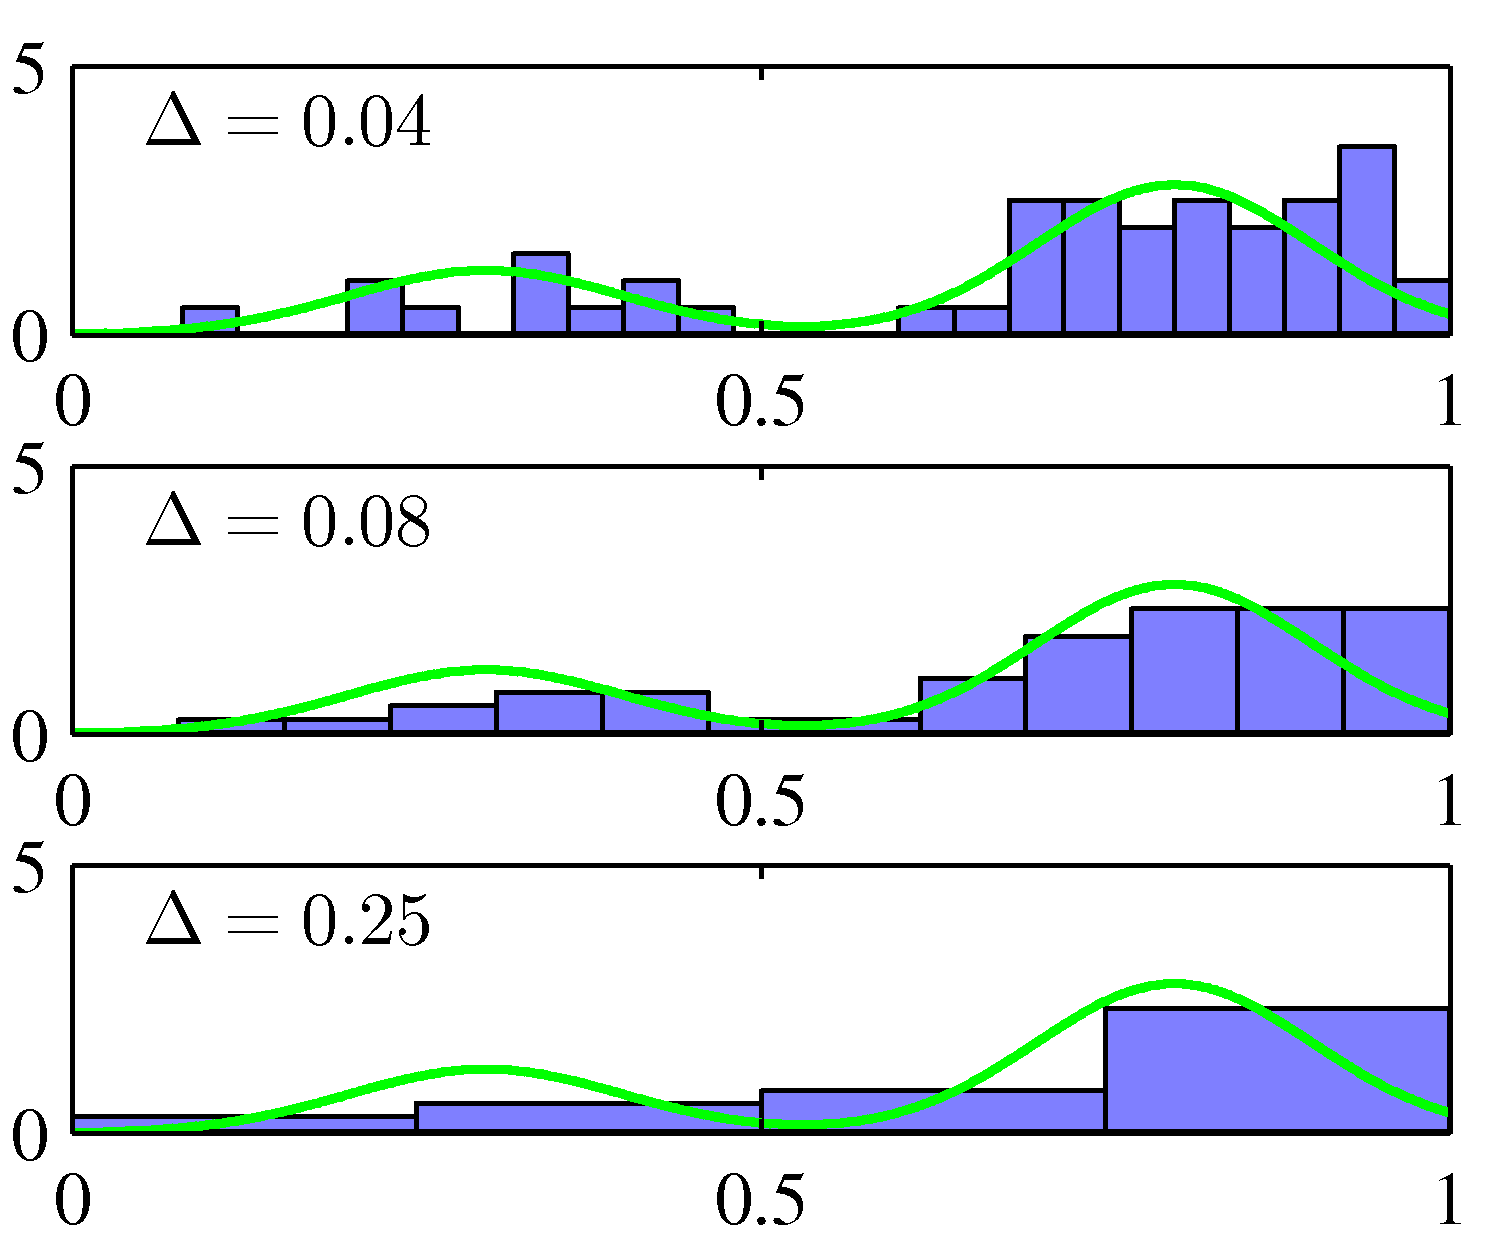
\includegraphics[scale=0.8]{Images/2-24.png}
		\captionsetup{font={small}}
		\caption{利用直方图方法进行概率密度估计的示例图,其中数据集包含了50组数据,全部的数据均来自于绿色曲线所示的分布。整个估计的过程是基于(2.241)的,将每个区域的宽度都设置了相同的值$\Delta$,并展示了$\Delta$取不同的值时直方图估计的结果。}
		\label{fig:2-24}
	\end{figure}
	\\
	\indent 需要注意的是,直方图方法具有一些后面即将讨论的方法所不具有的特点,一旦计算了直方图,数据集本身就可以被完全抛弃,这个特点对于较大的数据集无疑是很有利的。另外,对于顺序获取数据的情况,直方图方法也可以轻松应对。\\
	\indent 在实际应用中,直方图方法可以快速实现一维或二维数据的可视化,但对于大多数的概率密度估计问题,直方图方法可能无法应用。最明显的问题就是直方图方法估计得到的概率密度是不连续的,这个问题不随着生成数据的分布所具备的特性而改变,而是数据区域边缘所造成的固有缺陷。另外一个致命的限制是直方图方法的复杂度在维数发生变化时会急剧变化。如果将$D$维空间中的变量划分到$M$个区域中,那么区域的总数将是$M^D$。这样的指数型放大无疑是维数灾难的典型案例。在高维空间中,即使只是想要产生有效的局部概率密度估计,所需要的数据量也将是令人望而却步的。\\
	\indent 然而,直方图方法还教给我们两个重要的经验。首先,如果要估计某个特定位置的概率密度,我们应当考虑该点的局部邻域内其他数据的影响。注意,这里讨论的局部是指某种距离度量下的局部定义,而且这里先假设使用的是欧几里得距离。对于直方图而言,这个邻域的属性由区域定义,而且有一个自然"平滑"参数来描述这个局部区域的范围,也就是区域的宽度。其次,平滑参数不应选择得太大或太小。这很容易让人联想到第1章中讨论多项式曲线拟合问题时所说的模型复杂度选择的问题。其中的多项式次数$M$和正则化参数$\alpha$要取居中的值才能保证最佳的结果。带着这些见解,我们来讨论两种广泛使用的非参数密度估计方法,也就是核密度估计和最近邻方法。与简单的直方图方法比起来,它们对于维数变化具有更好的应对表现。
	}
	\subsection{核密度估计}
	\textnormal{假设我们的数据是从一个$D$维欧式空间中的未知概率密度$p(\bx)$中获取的,并希望利用这些数据来估计$p(\bx)$。根据前面关于局部性的讨论,我们需要考虑包含有$\bx$的小区域$\mathcal{R}$,在这个区域中的概率质量为
	\begin{equation}
		P = \int_{\calR} p(\bx) \ \rmd \bx
	\end{equation}
	现在假设我们有$N$组来自$p(\bx)$的数据,由于每个数据都有一个落入区域$\calR$的概率$P$,那么根据伯努利分布,落在$\calR$内的数据数量为$K$的概率为
	\begin{equation}
		\mathrm{Bin}(K|N,P)=\frac{N!}{K!(N-K)!}P^K(1-P)^{N-K}
	\end{equation}
	根据(2.11)可知,落入该区域的数据所占比例的均值为$\mathbb{E}[K/N]=P$,类似地,根据(2.12)可知在这个均值下的方差为$\mathrm{var}[K/N]=P(1-P)/N$。对于较大的$N$,这个分布将在均值附近形成尖锐的峰状,于是
	\begin{equation}
		K \approx NP
	\end{equation}
	然而,如果同时假设$\calR$充分小,以至于在某区域内概率密度$p(\bx)$可以近似为常数,那么可以得到
	\begin{equation}
		P \approx p(\bx)V
	\end{equation}
	其中$V$表示$\calR$的体积。结合(2.244)和(2.245),可以得到如下形式的概率密度估计
	\begin{equation}
		p(\bx)=\frac{K}{NV}
	\end{equation}
	然而(2.246)的正确与否取决于前面的两个自相矛盾的假设。一个假设是区域$\calR$必须充分小,使得区域内的概率密度近似为常数;另一个假设是区域相对于密度的值来说又足够大,使得落入该区域的数据数量$K$足以使二项分布急剧地达到峰值。\\
	\indent 我们有两种方式利用(2.246)。既可以用稍后即将讨论的K近邻方法(K-nearest-neighbour, KNN)对于固定的$K$根据数据确定$V$的值,也可以利用核方法(kernel)对于固定的$V$根据数据确定$K$。可以证明,当$N \rightarrow \infty$且$V$随着$N$适当收缩、$K$随着$N$适当增大时,KNN和核方法都可以收敛于真实的概率密度(Duda and Hart, 1973)。\\
	\indent 我们首先从核方法开始讨论,在初始阶段,我们认为区域$\calR$是一个中心为$\bx$的超立方体,而我们希望确定的就是$\bx$处的概率密度。为了计算落入该区域的数据数量$K$,定义如下的函数
	\begin{equation}
		k(\mathbf{u})=\begin{cases}
		1,&|u_i|\leqslant 1/2,\ i=1,...,D\\
		0,&\text{otherwise}
		\end{cases}
	\end{equation}
	这个函数表示的是一个中心位于原点的单位立方体。这里的$k(\mathbf{u})$就是一个核函数(kernel function),在现在这个背景下也被称为Parzen窗(Parzen window)。根据(2.247),如果数据点$\bx_n$落在以$\bx$为中心,$h$为边长的立方体中,那么$k((\bx-\bx_n)/h)$的值为1,否则为0。那么落在这个立方体中的数据数量为
	\begin{equation}
		K = \sum_{n=1}^N k\left(\frac{\bx-\bx_n}{h}\right)
	\end{equation}
	将这个表达式代入(2.246),于是可得$\bx$处的概率密度估计
	\begin{equation}
		p(\bx)=\frac{1}{N}\sum_{n=1}^N \frac{1}{h^D}k\left(\frac{\bx-\bx_n}{h}\right)
	\end{equation}
	其中用到了$D$维空间中边长为$h$的超立方体的体积$V=h^D$。根据函数$k(\mathbf{u})$的对称性,对于这个等式可以有一个新的解释,不再是一个以$\bx$为中心的单个立方体,而是以$N$个数据点$\bx_n$为中心的立方体的总和。\\
	\indent 到目前为止,核密度估计方法(2.249)仍然没有逃脱与直方图方法相同的严重问题,那就是人为造成的不连续性,在现在的方法中,不连续的位置是立方体的边缘处。不过如果我们选择更加平滑的核函数,得到的概率密度模型就会更加平滑。此时通常会选择高斯概率密度函数,对应的核密度模型为
	\begin{equation}
		p(\bx)=\frac{1}{N}\sum_{n=1}^N \frac{1}{(2 \pi h^2)^{D/2}}\exp\left\{-\frac{\|\bx-\bx_n\|^2}{2h^2}\right\}
	\end{equation}
	其中$h$表示高斯组件的标准差。所以我们的概率密度模型实际上是假设每个数据点都服从高斯分布,然后将所有的高斯分布叠加在一起,再除以$N$以确保满足归一化条件得到的。如图2.25所示,我们利用模型(2.250)估计此前用直方图方法估计过的概率密度。可以看出,参数$h$起到了平滑的作用,而且需要在过小和过大的$h$之间取一个折衷,过小会导致对噪声过度敏感,过大会导致估计过于平滑。同样地,$h$的优化是一个模型复杂度的问题,类似于直方图概率密度估计中的区域宽度,或者多项式曲线拟合问题中多项式的复杂度。
	\begin{figure}[ht]
		\centering
		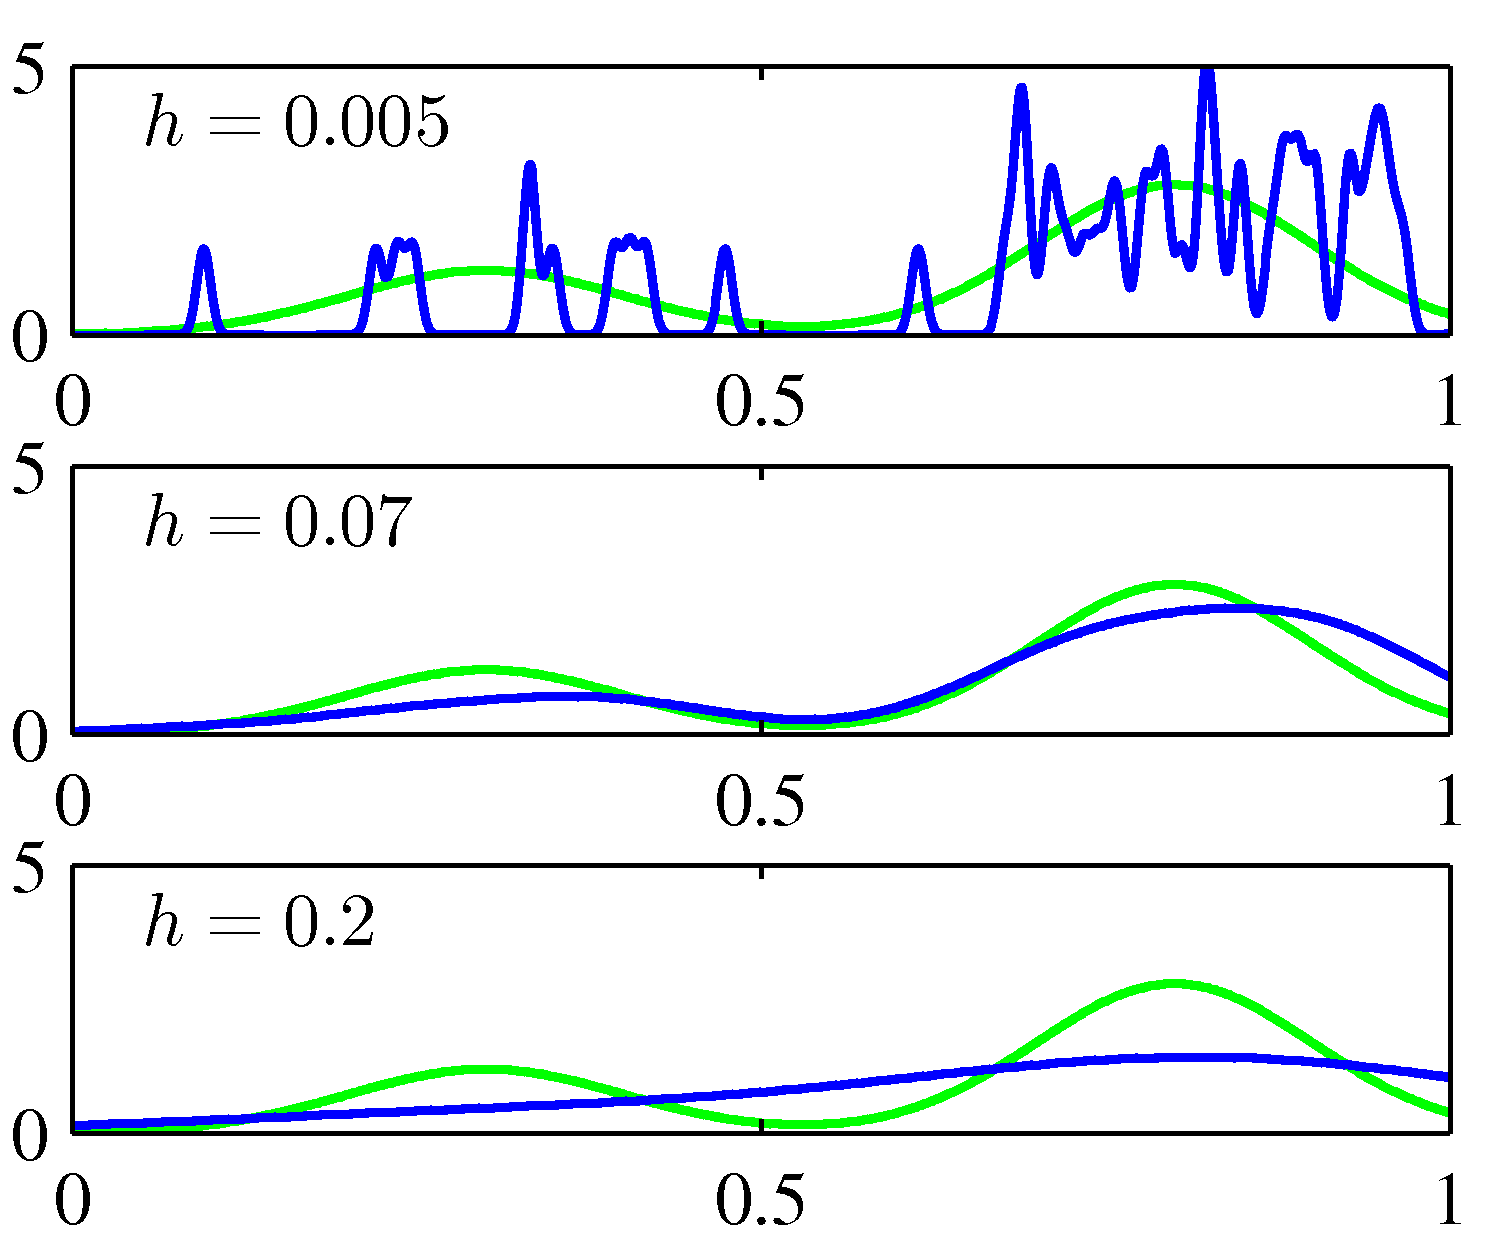
\includegraphics[scale=0.8]{Images/2-25.png}
		\captionsetup{font={small}}
		\caption{对于图2.24中的数据集采用核密度模型(2.250)进行估计的结果。可以看出,$h$充当了平滑系数的角色,如果$h$过小(最上方图片),那么密度模型将是极其混乱的;但如果$h$过大(最下方图片),又无法描述出原分布(绿色曲线)具有双峰值的特点。采用适中的$h$值(中间图片)则可以得到较好的密度模型。}
		\label{fig:2-25}
	\end{figure}
	\\
	\indent 对于(2.249),我们可以选择任意的核函数$k(\mathbf{u})$,但要满足条件
	\begin{align}
		k(\mathbf{u}) &\geqslant 0 \\
		\int k(\mathbf{u})\ \rmd \mathbf{u} &= 1
	\end{align}
	也就是概率分布必须满足的非负性和归一性。(2.249)这样的一类密度模型称为核密度估计,也叫作Parzen估计。这个方法具有很大的优点,即“训练”阶段不需要进行计算,只需要把训练集存下来就可以。然而,这也正是最大的缺陷之一,因为评估概率密度的计算成本随着数据集数量的增大而线性增长。
	}
	\subsection{近邻方法}
	\textnormal{
	在概率密度估计中使用核方法的一大困难就是控制核宽度的参数$h$对于所有的核来说都必须是固定的。在数据密度较高的区域中,如果$h$选得较大,可能会导致估计的过度平滑,破坏了本该从数据中分析出来的结构。然而要是减小$h$,又会导致在数据密度较小的区域中形成很混乱的估计结果。在概率密度估计的近邻方法中,这个问题得到了有效的解决。\\
	\indent 再次回到局部概率密度估计(2.246),这次不再固定$V$来确定$K$,而是固定$K$来确定$V$。为了做到这一点,我们假设有一个以$\bx$为中心的小球体,而我们希望确定的就是$\bx$处的概率密度$p(\bx)$,并允许球体的半径增加到准确包含了$K$个数据点为止。那么这样得到的密度估计$p(\bx)$仍然是(2.246),其中的$V$是球体最终的体积。这个方法称为$K$近邻方法($K$ nearest neighbours),在参数$K$的不同取值下,利用K近邻方法估计与图2.24、图2.25相同的数据集的结果如图2.26所示。可以看出参数$K$控制了平滑度,而且同样也是不宜过大或过小。需要注意的是,根据$K$近邻方法得到的模型并不是一个真实的概率密度模型,因为它在完整空间上的积分是发散的。\textcolor{red}{\textbf{——习题 2.61}}
	\begin{figure}[ht]
		\centering
		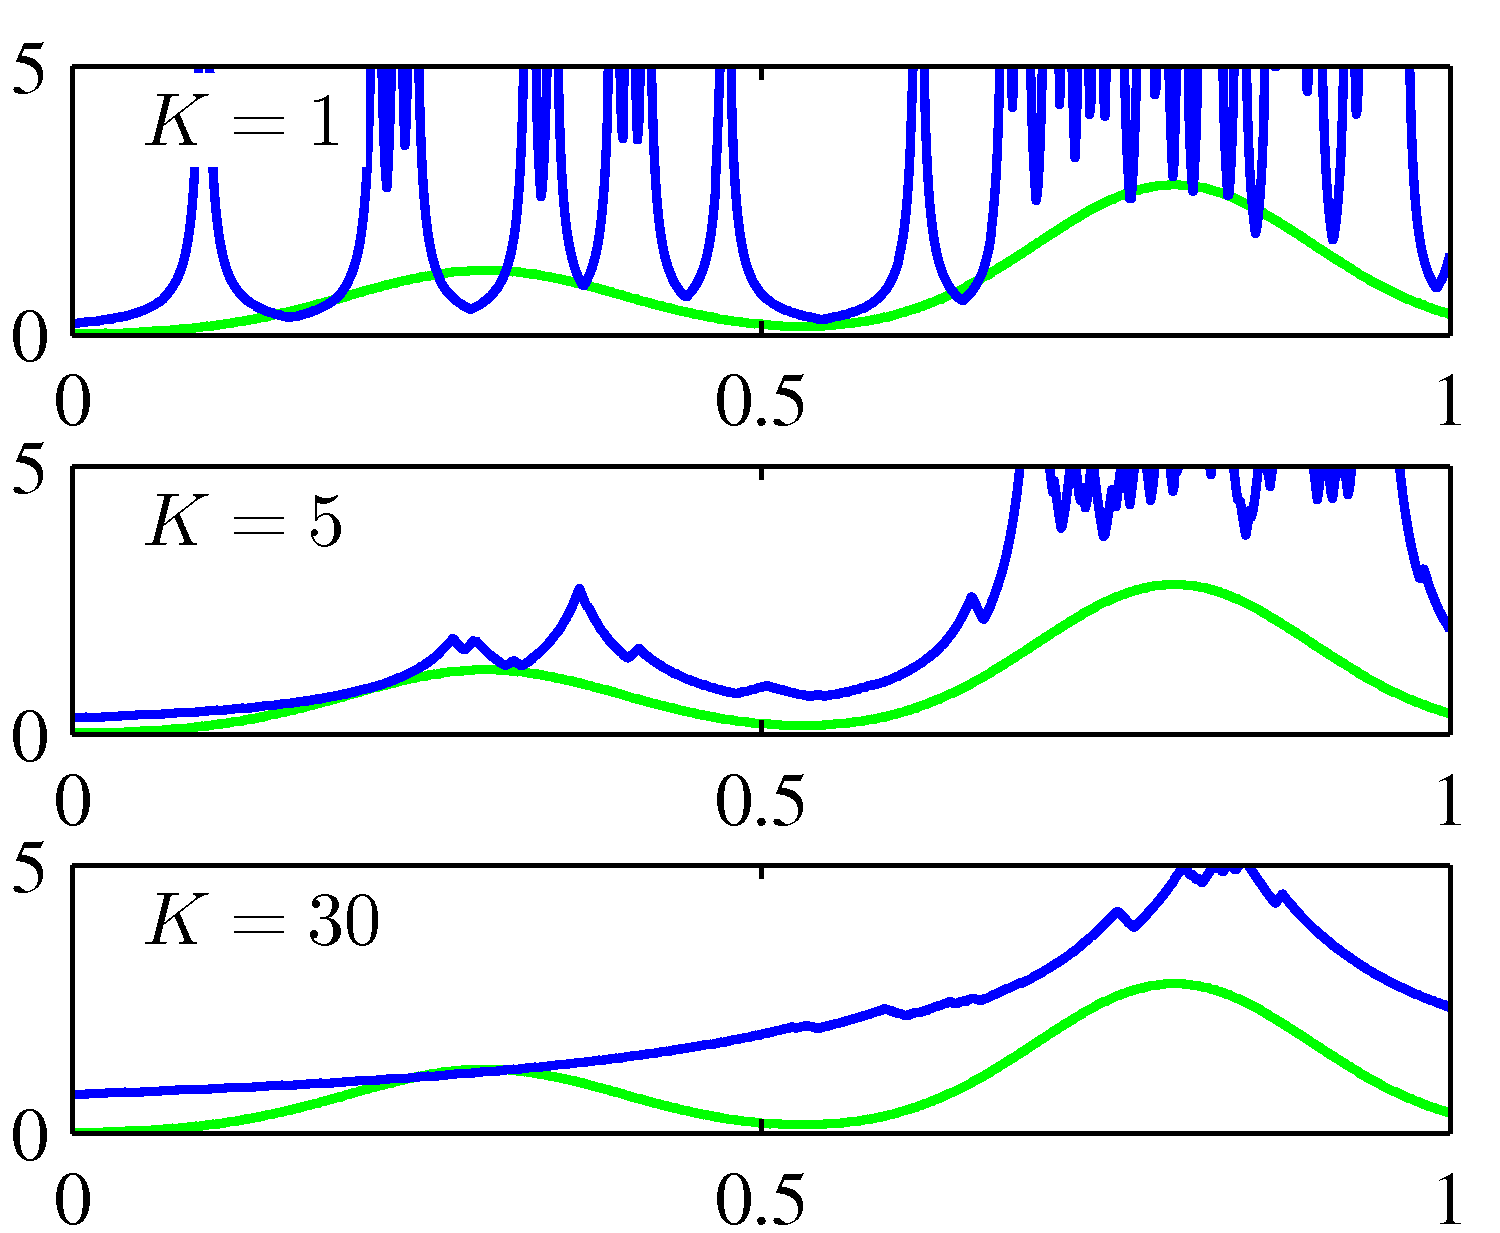
\includegraphics[scale=0.8]{Images/2-26.png}
		\captionsetup{font={small}}
		\caption{利用$K$近邻方法处理与图2.24和2.25相同的数据集的结果。可以看出,参数$K$控制了平滑度,所以较小的$K$(最上方的图)会使模型变得混乱,较大的$K$(最下方的图)会使得估计结果体现不出原分布具有两个峰值这一特点。}
		\label{fig:2-26}
	\end{figure}
	\\
	\indent 在本章的最后,我们证明一下概率密度估计的$K$近邻方法可以扩展到分类问题中。在证明中,我们对于每个类别分别进行$K$近邻密度估计,并利用了贝叶斯定理。假设数据集中属于类别$\mathcal{C}_k$的数据数量为$N_k$,数据总数为$N$,那么$\sum_k N_k =N$。在对一个新的数据$\bx$分类时,我们以$\bx$为中心,画一个包含了$K$个数据点的球体——此时忽略这些数据点的类别,只管数量。假设这个球体的体积为$V$,且其中包含了$K_k$个属于类别$\mathcal{C}_k$的数据。那么根据(2.246)可以写出每个类别对应的密度估计
	\begin{equation}
		p(\bx|\mathcal{C}_k)=\frac{K_k}{N_k V}
	\end{equation}
	类似地,不带条件的概率密度为
	\begin{equation}
		p(\bx)=\frac{K}{NV}
	\end{equation}
	且分类的先验为
	\begin{equation}
		p(\mathcal{C}_k)=\frac{N_k}{N}
	\end{equation}
	利用贝叶斯定理将(2.253),(2.254)和(2.255)结合起来,于是可以得到分类的后验概率
	\begin{equation}
		p(\mathcal{C}_k|\bx)=\frac{p(\bx|\mathcal{C}_k)p(\mathcal{C}_k)}{p(\bx)} = \frac{K_k}{K}
	\end{equation}
	\indent 如果希望将分类错误的概率最小化,那么就应该为$\bx$指派后验概率最大的那个类别,而最大后验概率就是$K_k/K$的最大值。所以,如果想要将一个新的数据点进行分类,我们需要从数据集中取出$K$个距离它最近的数据,并认为这些数据中数量最多的那个类别就是这个新数据点的类别。当然规则是可以变化的,$K=1$时称为最近邻规则,因为在这种情况下将直接把与测试点最近的训练点的类别赋予测试点。图2.27展示了这些概念。图2.28中所示的是利用$K$近邻方法处理第1章中油流数据集的结果。不出意料,$K$控制了平滑度,如果$K$较小,那么会出现很多小的分类区域,而如果$K$较大,分类区域的范围就变得比较大了。
	\begin{figure}[ht]
		\begin{minipage}[t]{0.5\linewidth}
		\centering
		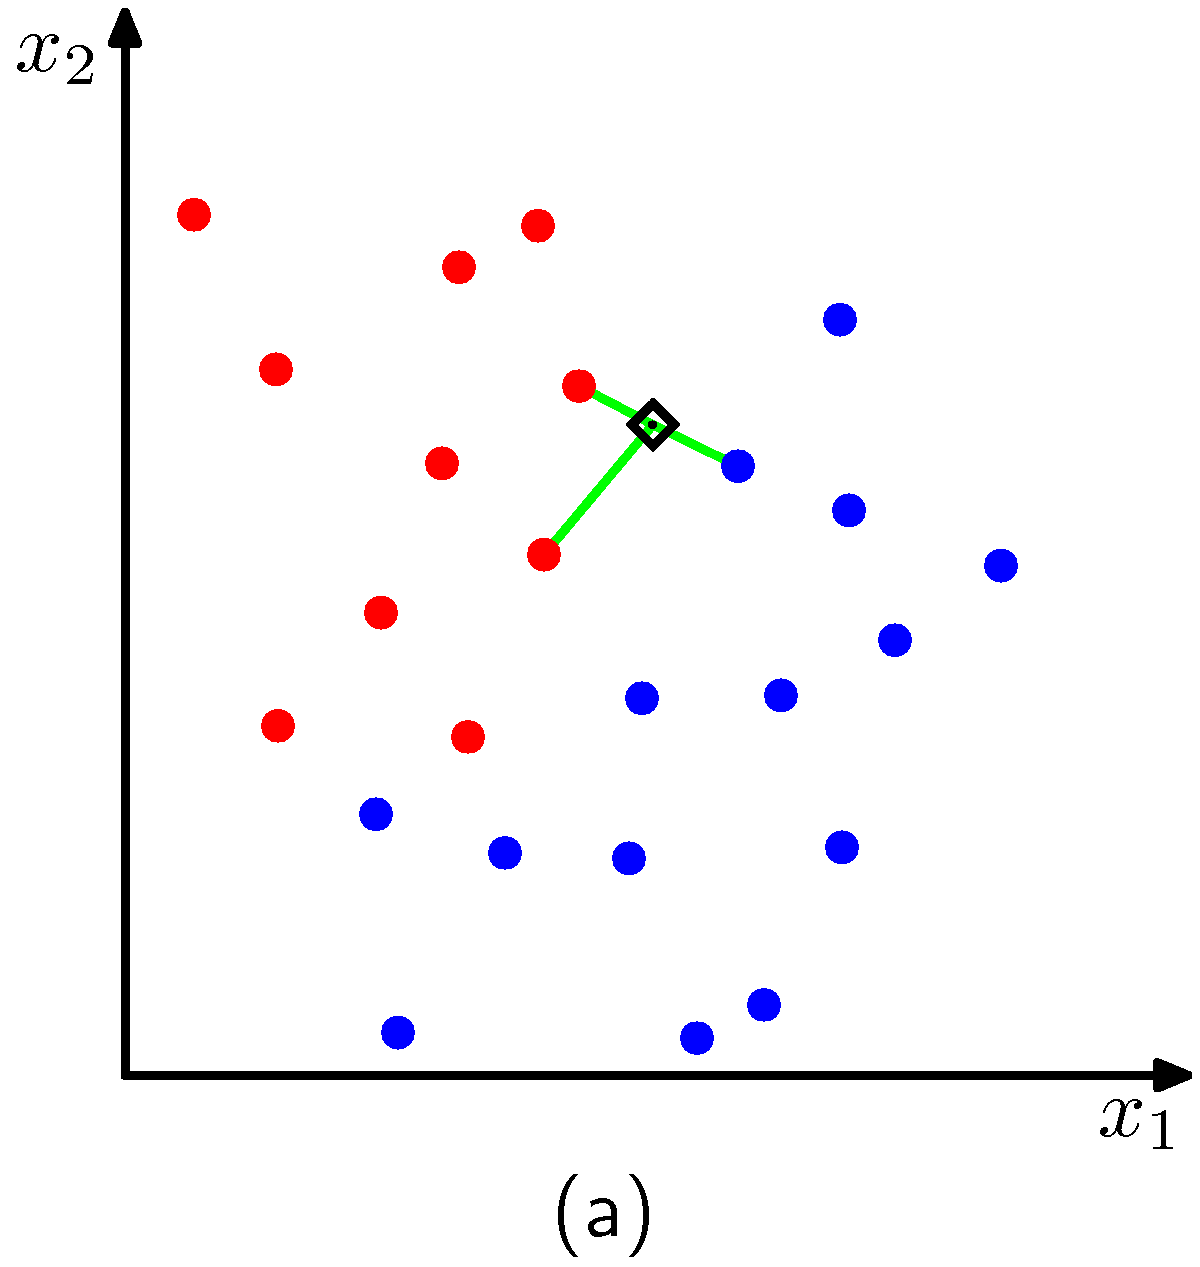
\includegraphics[scale=0.8]{Images/2-27a.png}
		\label{fig:2-27a}
		\end{minipage}
		\begin{minipage}[t]{0.5\linewidth}
		\centering
		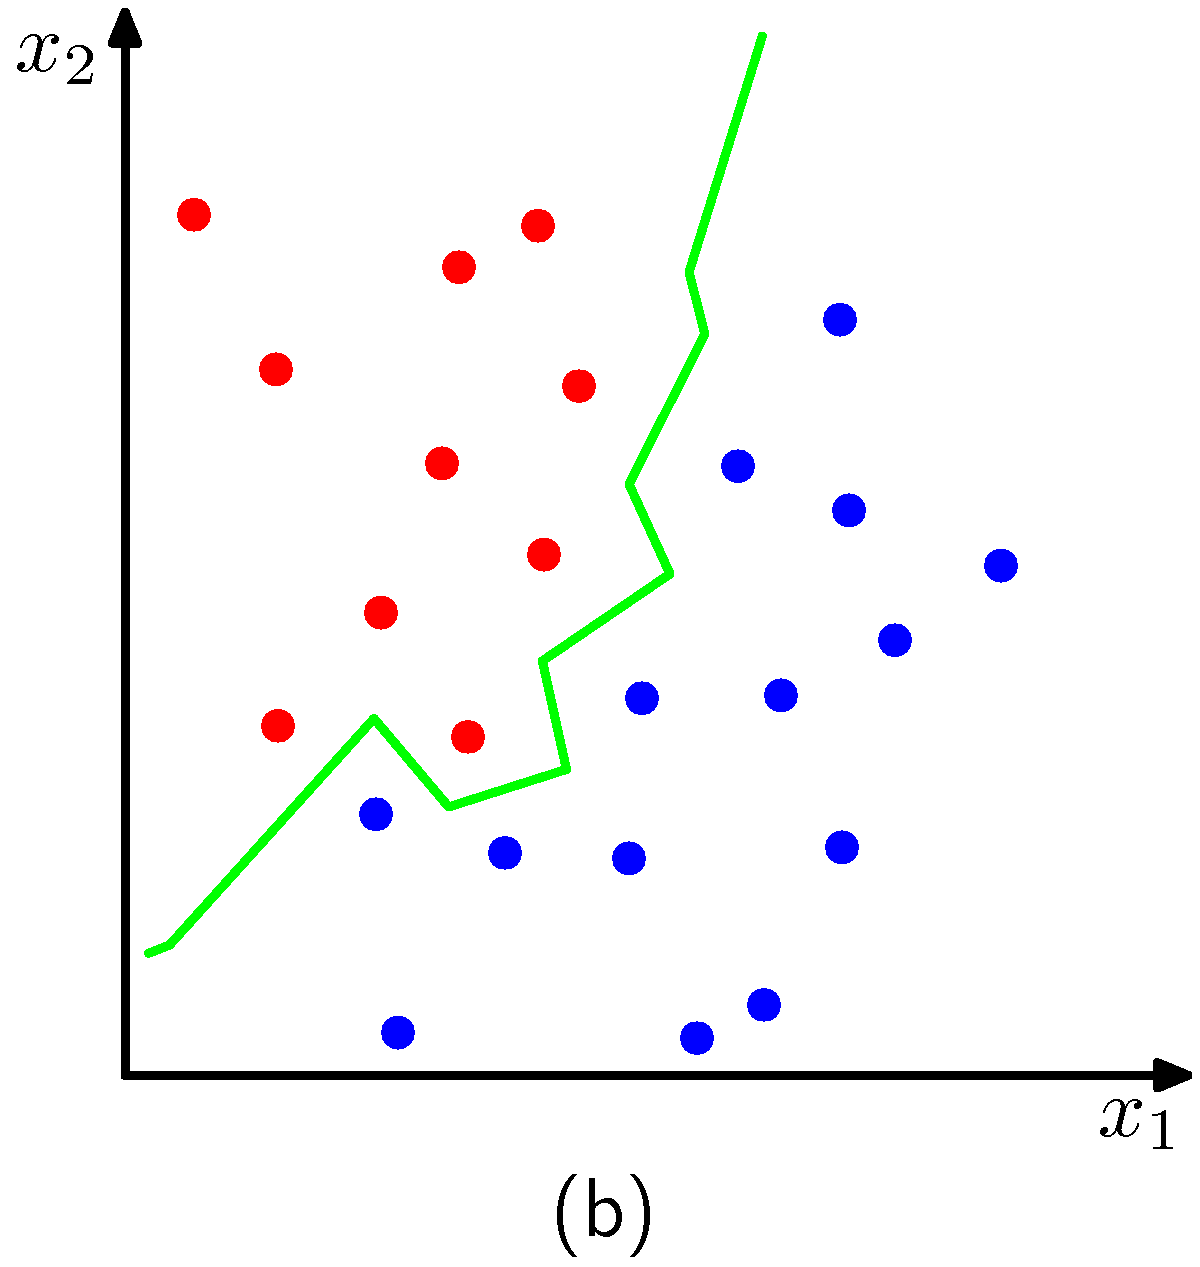
\includegraphics[scale=0.8]{Images/2-27b.png}
		\label{fig:2-27b}
		\end{minipage}
		\captionsetup{font={small}}
		\caption{(a)\ 在$K$近邻分类中,新数据(黑色方块)的类别将根据与其最近的$K$个训练数据的类别确定。(b)\ 在最近邻分类($K=1$)中,得到的决策界由超平面组成,这些超平面是一对不同类别的数据之间连线的垂直平分线。}
		\begin{minipage}[t]{0.3\linewidth}
		\centering
		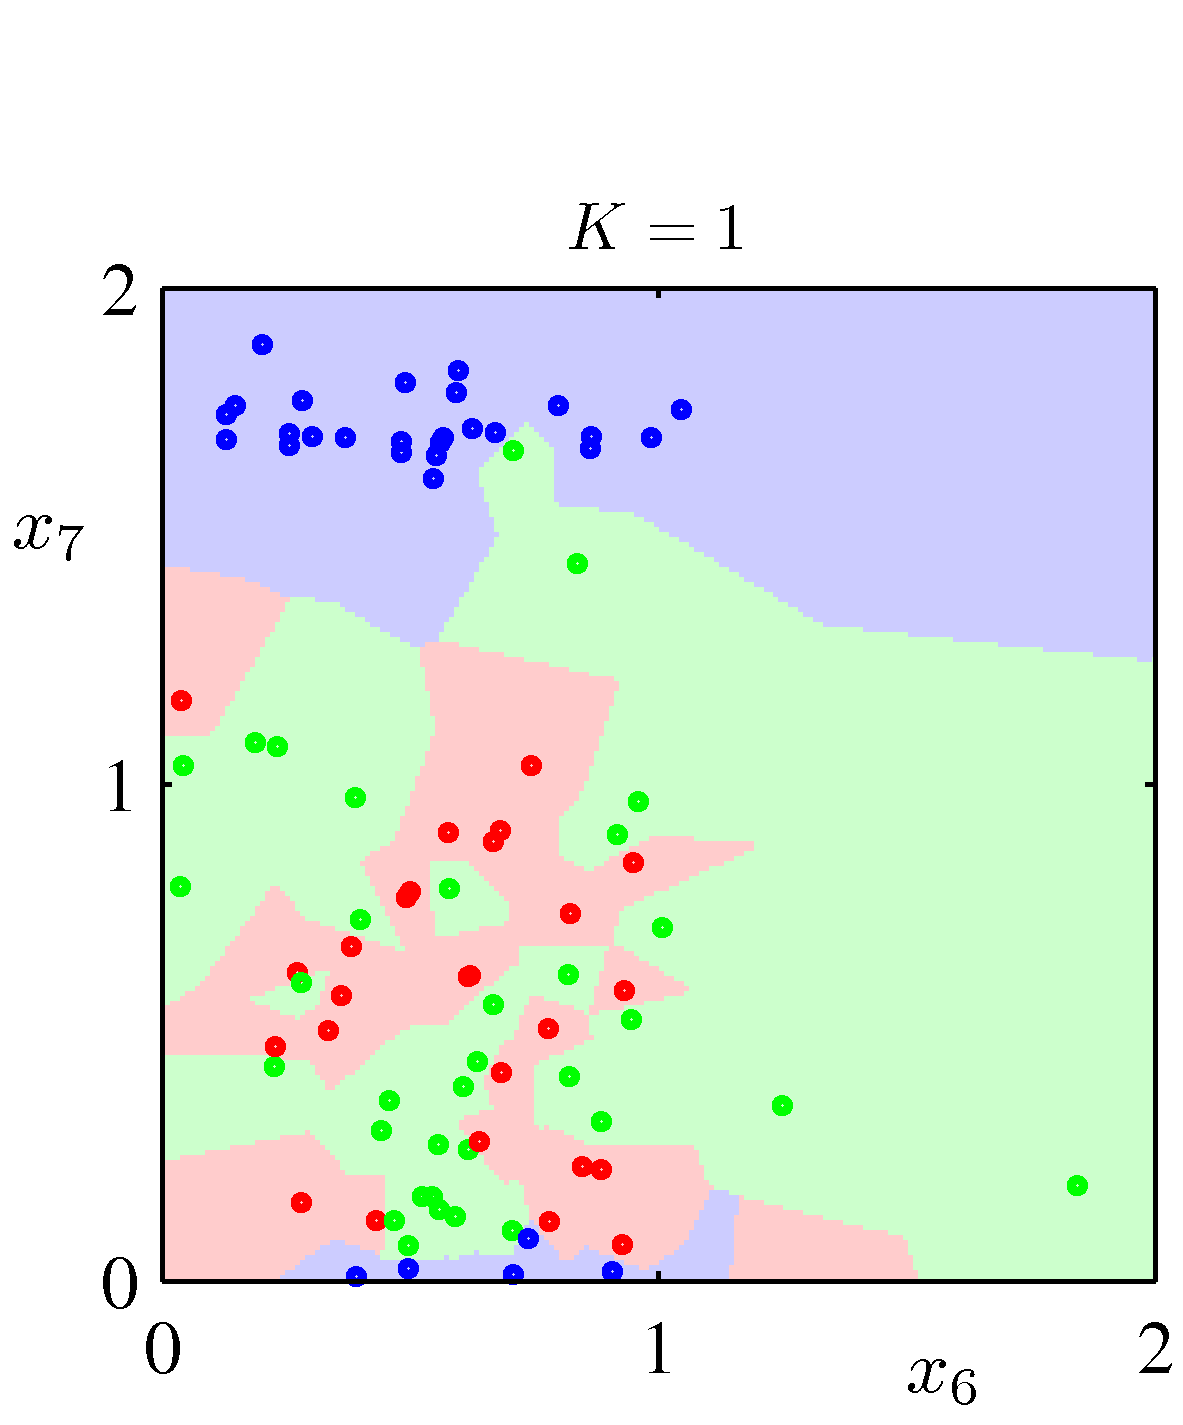
\includegraphics[scale=0.8]{Images/2-28a.png}
		\label{fig:2-28a}
		\end{minipage}
		\begin{minipage}[t]{0.3\linewidth}
		\centering
		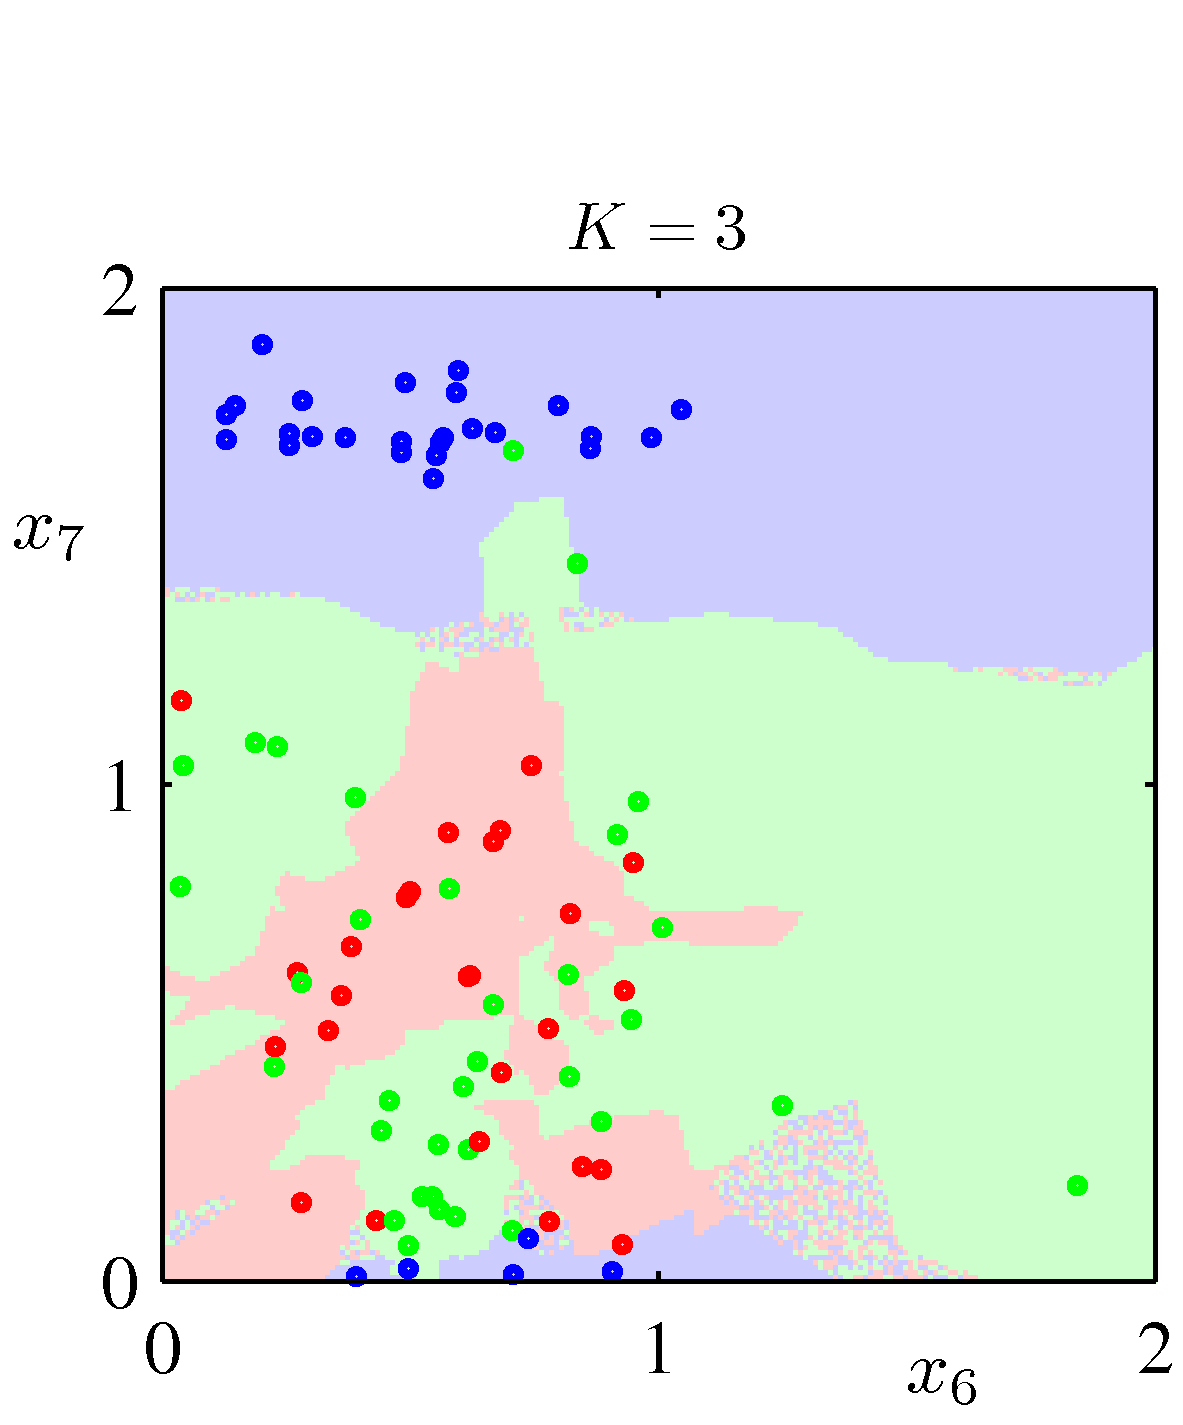
\includegraphics[scale=0.8]{Images/2-28b.png}
		\label{fig:2-28b}
		\end{minipage}
		\begin{minipage}[t]{0.3\linewidth}
		\centering
		\includegraphics[scale=0.8]{Images/2-28c.png}
		\label{fig:2-28c}
		\end{minipage}
		\captionsetup{font={small}}
		\caption{油流数据集中200个数据的$x_6$和$x_7$,其中红色、绿色和蓝色分别表示“层状物”,“环状物”和“层状物”,并给出了不同$K$值下利用$K$近邻算法进行输入空间分类的结果。}
	\end{figure}
	\\
	\indent 最近邻分类($K=1$)有一个很有意思的特性,在极限$N \rightarrow \infty$下,其错误率将永远不高于最优分类器(即真实分布)错误率的2倍。在目前的讨论中,不论是$K$近邻方法还是核方法,都要求存储完整的数据集,在数据集较大时,无疑会导致计算压力过大。通过构造基于树的搜索结构,可以(近似地)发现临近的数据,而不需要穷举检索,这样做可以稍微缓解一下这个问题,但代价是需要一些额外的一次性计算。然而,这些非参数方法仍然受到严重的限制。另一方面,简单的参数模型能够表示的分布形式又具有很大的局限性。因此,我们需要非常灵活的概率密度模型而且要使模型的复杂度与训练集的大小无关。我们将在后续章节中看到如何做到这些。
	}
\end{document}